\documentclass[a4paper,11pt,twoside]{ThesisStyle}

\usepackage{amsmath,amssymb}             % AMS Math
% \usepackage[french]{babel}
\usepackage[latin1]{inputenc}
\usepackage[T1]{fontenc}
\usepackage[left=1.5in,right=1.3in,top=1.1in,bottom=1.1in,includefoot,includehead,headheight=13.6pt]{geometry}
\renewcommand{\baselinestretch}{1.05}

% Table of contents for each chapter

\usepackage[nottoc, notlof, notlot]{tocbibind}
\usepackage{minitoc}
\setcounter{minitocdepth}{2}
\mtcindent=15pt
% Use \minitoc where to put a table of contents

\usepackage{aecompl}

% Glossary / list of abbreviations

\usepackage[intoc]{nomencl}
\renewcommand{\nomname}{List of Abbreviations}

\makenomenclature

% My pdf code

\usepackage{ifpdf}

\ifpdf
  \usepackage[pdftex]{graphicx}
  \DeclareGraphicsExtensions{.jpg}
  \usepackage[a4paper,pagebackref,hyperindex=true]{hyperref}
\else
  \usepackage{graphicx}
  \DeclareGraphicsExtensions{.ps,.eps}
  \usepackage[a4paper,dvipdfm,pagebackref,hyperindex=true]{hyperref}
\fi

\graphicspath{{.}{images/}}

% nicer backref links
\renewcommand*{\backref}[1]{}
\renewcommand*{\backrefalt}[4]{%
\ifcase #1 %
(Not cited.)%
\or
(Cited on page~#2.)%
\else
(Cited on pages~#2.)%
\fi}
\renewcommand*{\backrefsep}{, }
\renewcommand*{\backreftwosep}{ and~}
\renewcommand*{\backreflastsep}{ and~}

% Links in pdf
\usepackage{color}
\definecolor{linkcol}{rgb}{0,0,0.4} 
\definecolor{citecol}{rgb}{0.5,0,0} 

% Change this to change the informations included in the pdf file

% See hyperref documentation for information on those parameters

\hypersetup
{
bookmarksopen=true,
pdftitle="Design and Use of Anatomical Atlases for Radiotherapy",
pdfauthor="Olivier COMMOWICK", 
pdfsubject="Creation of atlases and atlas based segmentation", %subject of the document
%pdftoolbar=false, % toolbar hidden
pdfmenubar=true, %menubar shown
pdfhighlight=/O, %effect of clicking on a link
colorlinks=true, %couleurs sur les liens hypertextes
pdfpagemode=None, %aucun mode de page
pdfpagelayout=SinglePage, %ouverture en simple page
pdffitwindow=true, %pages ouvertes entierement dans toute la fenetre
linkcolor=linkcol, %couleur des liens hypertextes internes
citecolor=citecol, %couleur des liens pour les citations
urlcolor=linkcol %couleur des liens pour les url
}

% definitions.
% -------------------

\setcounter{secnumdepth}{3}
\setcounter{tocdepth}{2}

% Some useful commands and shortcut for maths:  partial derivative and stuff

\newcommand{\pd}[2]{\frac{\partial #1}{\partial #2}}
\def\abs{\operatorname{abs}}
\def\argmax{\operatornamewithlimits{arg\,max}}
\def\argmin{\operatornamewithlimits{arg\,min}}
\def\diag{\operatorname{Diag}}
\newcommand{\eqRef}[1]{(\ref{#1})}

\usepackage{rotating}                    % Sideways of figures & tables
%\usepackage{bibunits}
%\usepackage[sectionbib]{chapterbib}          % Cross-reference package (Natural BiB)
%\usepackage{natbib}                  % Put References at the end of each chapter
                                         % Do not put 'sectionbib' option here.
                                         % Sectionbib option in 'natbib' will do.
\usepackage{fancyhdr}                    % Fancy Header and Footer

\usepackage{txfonts}                     % Public Times New Roman text & math font
  
%%% Fancy Header %%%%%%%%%%%%%%%%%%%%%%%%%%%%%%%%%%%%%%%%%%%%%%%%%%%%%%%%%%%%%%%%%%
% Fancy Header Style Options

\pagestyle{fancy}                       % Sets fancy header and footer
\fancyfoot{}                            % Delete current footer settings

%\renewcommand{\chaptermark}[1]{         % Lower Case Chapter marker style
%  \markboth{\chaptername\ \thechapter.\ #1}}{}} %

%\renewcommand{\sectionmark}[1]{         % Lower case Section marker style
%  \markright{\thesection.\ #1}}         %

\fancyhead[LE,RO]{\bfseries\thepage}    % Page number (boldface) in left on even
% pages and right on odd pages
\fancyhead[RE]{\bfseries\nouppercase{\leftmark}}      % Chapter in the right on even pages
\fancyhead[LO]{\bfseries\nouppercase{\rightmark}}     % Section in the left on odd pages

\let\headruleORIG\headrule
\renewcommand{\headrule}{\color{black} \headruleORIG}
\renewcommand{\headrulewidth}{1.0pt}
\usepackage{colortbl}
\arrayrulecolor{black}

\fancypagestyle{plain}{
  \fancyhead{}
  \fancyfoot{}
  \renewcommand{\headrulewidth}{0pt}
}

\usepackage{algorithm}
\usepackage[noend]{algorithmic}

%%% Clear Header %%%%%%%%%%%%%%%%%%%%%%%%%%%%%%%%%%%%%%%%%%%%%%%%%%%%%%%%%%%%%%%%%%
% Clear Header Style on the Last Empty Odd pages
\makeatletter

\def\cleardoublepage{\clearpage\if@twoside \ifodd\c@page\else%
  \hbox{}%
  \thispagestyle{empty}%              % Empty header styles
  \newpage%
  \if@twocolumn\hbox{}\newpage\fi\fi\fi}

\makeatother
 
%%%%%%%%%%%%%%%%%%%%%%%%%%%%%%%%%%%%%%%%%%%%%%%%%%%%%%%%%%%%%%%%%%%%%%%%%%%%%%% 
% Prints your review date and 'Draft Version' (From Josullvn, CS, CMU)
\newcommand{\reviewtimetoday}[2]{\special{!userdict begin
    /bop-hook{gsave 20 710 translate 45 rotate 0.8 setgray
      /Times-Roman findfont 12 scalefont setfont 0 0   moveto (#1) show
      0 -12 moveto (#2) show grestore}def end}}
% You can turn on or off this option.
% \reviewtimetoday{\today}{Draft Version}
%%%%%%%%%%%%%%%%%%%%%%%%%%%%%%%%%%%%%%%%%%%%%%%%%%%%%%%%%%%%%%%%%%%%%%%%%%%%%%% 

\newenvironment{maxime}[1]
{
\vspace*{0cm}
\hfill
\begin{minipage}{0.5\textwidth}%
%\rule[0.5ex]{\textwidth}{0.1mm}\\%
\hrulefill $\:$ {\bf #1}\\
%\vspace*{-0.25cm}
\it 
}%
{%

\hrulefill
\vspace*{0.5cm}%
\end{minipage}
}

\let\minitocORIG\minitoc
\renewcommand{\minitoc}{\minitocORIG \vspace{1.5em}}

\usepackage{multirow}
\usepackage{slashbox}

\newenvironment{bulletList}%
{ \begin{list}%
	{$\bullet$}%
	{\setlength{\labelwidth}{25pt}%
	 \setlength{\leftmargin}{30pt}%
	 \setlength{\itemsep}{\parsep}}}%
{ \end{list} }


\renewcommand{\epsilon}{\varepsilon}

% centered page environment

\newenvironment{vcenterpage}
{\newpage\vspace*{\fill}\thispagestyle{empty}\renewcommand{\headrulewidth}{0pt}}
{\vspace*{\fill}}


\usepackage{dsfont,,epsfig,psfrag,stmaryrd,amsfonts,mathrsfs,booktabs,algorithmic} % Add all your packages here
\usepackage{alltt}
\usepackage[standard]{ntheorem}
%\usepackage{floatflt}
%\usepackage{caption}
%\usepackage[font=footnotesize,caption]{subfig}
\usepackage{array}
\renewcommand{\theequation}{\arabic{equation}}
\usepackage{subfigure}






\newcommand{\JFC}[1]{\begin{color}{green}\textit{#1}\end{color}}
\newcommand{\CG}[1]{\begin{color}{blue}\textit{#1}\end{color}}

\newcommand{\Fig}[1]{Fig.~\ref{#1}}
\newcommand{\Algo}[1]{\textbf{\ref{#1}}}




\begin{document}

\begin{titlepage}

% $\raise\baselineskip\hbox{
%    \vtop to0pt{%
%       \hbox{}\hbox to0pt{
\includegraphics[scale=0.14]{tlloria}\hss}\vss}%
% }$\hskip2.5cm%




\begin{center}

\noindent {\large \textbf{UNIVERSITY OF FRANCHE-COMTE}} \\
\vspace*{0.3cm}
\noindent {\LARGE \textbf{DOCTORAL SCHOOL SPIM}} \\
\noindent \textbf{LABORATOIRE D'INFORMATIQUE DE L'UNIVERSITE DE FRANCHE-COMTE\\ (LIFC) } \\
\vspace*{0.5cm}
\noindent \Huge \textbf{P H D\ \ T H E S I S} \\
\vspace*{0.3cm}
\noindent \large {to obtain the title of} \\
\vspace*{0.3cm}
\noindent \LARGE \textbf{PhD of Science} \\
\vspace*{0.3cm}
\noindent \Large of the University of Franche-Comte \\
\noindent \Large \textbf{Specialty : \textsc{Computer Science}}\\
\vspace*{0.4cm}
\noindent \large {Defended by\\}
\noindent \LARGE Qianxue \textsc{WANG} \\
\vspace*{0.8cm}
\noindent {\Huge \textbf{Generating pseudo-random numbers. Applications in cryptology}} \\
\vspace*{0.8cm}
\noindent \Large Thesis Advisor:  Jacques \textsc{Bahi} \\
\vspace*{0.2cm}
\noindent \Large prepared at Numerical and Distributed Algorithms: \textsc{AND} Team\\
\vspace*{0.2cm}
\noindent \large defended on February 28, 2011 \\
\vspace*{0.5cm}
\end{center}
\noindent \large \textbf{Jury :} \\
\begin{center}
\noindent \large 
\begin{tabular}{llcl}
      \textit{Reviewers :}	&   \textsc{ }		& - &   \\
				&   \textsc{ }		& - &  \\
      \textit{Advisor :}	&  \textsc{}		& - &  \\
      \textit{President :}	&  \textsc{}		& - & \\
      \textit{Examinators :}   &  \textsc{}          & - & \\
      				&  \textsc{}			& - & \\
      				& \textsc{}		& - & \\
      \textit{Invited :}		&  \textsc{}		& - & 
\end{tabular}
\end{center}

% \newcommand{\@NancyIhe@d}{{\UseEntryFont{ThesisFirstPageHead}\noindent
%     \centerline{\if@logo@uhp@
%                     {\setbox0=\hbox{$\raise2.5cm\hbox{\UHPLogo}$}%
%                      \ht0=\baselineskip\box0}\hfill
%                 \else
%                     Universit\'e Henri Poincar\'e -- Nancy 1%
%                 \fi}%
%     \@TL@cmn@head\\
%     UFR ST\par
%     }%
%     }
% \hbox{$\raise2.5cm\hbox{\vtop to0pt{\hbox{}\hbox to0pt{
\includegraphics[scale=0.2]{tluhp}\hss}\vss}$}

\end{titlepage}
\sloppy

\titlepage


\dominitoc

\pagenumbering{roman}

 \cleardoublepage

\section*{Acknowledgments}

Last thing to do :-)

% Technical support from Le m\'esocentre de calcul de Franche-Comt\'e is gratefully acknowledged. 
% We are also grateful to Xiaole Fang for the calculations of Comparative test parameters and Kamel Mazouzi for his helpful comments on cluster computing.

\tableofcontents

\mainmatter

\chapter{Introduction}
\label{Introduction}
\minitoc

The development and popularity of the Internet and its recent role in everyday life implies the need to protect data and privacy in digital world. This development has revealed new major security issues. For example, new security concerns have recently appeared because of the evolution of the Internet to support such activities as e-Voting, VoD, and digital rights management~\cite{Zhu200675}. Pseudorandom number generators (PRNGs) play an important role in all of these emerging techniques, because they are fundamental in cryptosystems and information hiding schemes. 

PRNGs are typically defined by a deterministic recurrent sequence in a finite state space, usually a finite field or ring, and an output function mapping each state to an input value. 
This is often either a real number in the interval $(0,1)$ or an integer in some finite range~\cite{LEcuyer08}. 
Indeed, the generated sequence is not truly random, as it is completely determined by a relatively small set of initial values, called the PRNG's state space. 
Compared to hardware-based approaches, these PRNGs are more easy to generate and process, they are reproducible, but nevertheless are less closer to truly random behavior. 
PRNGs are often based on logical operations like bitwise exclusive or (XOR) and on circular shift of bit vectors. 
However the security level of some PRNGs of this kind has revealed to be inadequate by today's standards. 

Recently, some researchers have explored the possibility to use chaotic dynamical systems as PRNGs~\cite{Falcioni2005,Cecen2009,PO2004}. 
These attempts are due to the hypothesis that digital chaotic systems can possibly reinforce the security of cryptographic algorithms, because the behaviors of chaotic dynamical systems are very similar to those of physical noise sources~\cite{Schuster1984}. 
Their sensitivity to initial conditions and their broadband spectrum make them good candidates to generate cryptographically secure PRNGs. Particularly,  
the random-like, unpredictable dynamics of chaotic systems, their inherent determinism and simplicity of realization suggest their potential for exploitation as PRNGs.

In chaotic cryptography, there are two main design paradigms: in the first
paradigm chaotic cryptosystems are realized in analog circuits (mainly based on
chaos synchronization technique)~\cite{PhysRevLett.64.821}, and in the second paradigm chaotic cryptosystems
are realized in digital circuits or computers and do not depend on
chaos synchronization technique. Generally speaking, synchronization based
chaotic cryptosystems are generally designed for secure communications though
noisy channels and cannot directly extended to design digital ciphers in pure
cryptography. What's worse, many cryptanalytic works have shown that most
synchronization based chaotic cryptosystems are not secure since it is possible
to extract some information on secure chaotic parameters~\cite{BethLaMa94}. Therefore,
although chaos synchronization is still actively studied in research of secure
communications, the related ideas have less significance for conventional cryptographers.
Since this dissertation is devoted to research lying between chaotic
cryptography and traditional cryptography, only digital chaotic ciphers will be
discussed in this dissertation.

However, even though chaotic systems exhibit
random-like behavior, they are not necessarily cryptographically secure in their discretized
form, see e.g. ~\cite{HabutsuNSM91,Biham91cryptanalysisof}. The reason partly being that discretized chaotic functions do not automatically
yield sufficiently complex behavior of the corresponding binary functions, which is
a prerequisite for cryptographic security. It is therefore essential that the complexity of the
binary functions is considered in the design phase such that necessary modifications can be
made. Moreover, many suggested PRNG based on chaos suffer from reproducibility problems
of the keystream due to the different handling of floating-point numbers on various processors,
see e.g. ~\cite{Matthews:1984}.

Chaotic dynamical systems are usually continuous and hence defined on the real numbers domain. The transformation from real numbers to integers may lead to the loss of the chaotic behavior. The conversion to integers needs a rigorous theoretical foundation.

In this paper, some new chaotic pseudo-random bit generator is presented, which can also be used to obtain numbers uniformly distributed between 0 and 1. Indeed, these bits can be grouped $n$ by $n$, to obtain the floating part of $x \in [0,1]$ represented in binary numeral system. These generators are based on discrete chaotic iterations which satisfy Devaney's definition of chaos~\cite{guyeux09}. A rigorous  framework is introduced, where topological chaotic properties of the generator are shown. 

The design goal of  these generators was to take advantage of the random-like properties of realvalued
chaotic maps and, at the same time, secure optimal cryptographic properties. More precisely, the design was initiated by constructing a chaotic system
on the integers domain instead of the real numbers domain.

The quality of a PRNG is proven both by theoretical foundations and empirical validations. 
Various statistical tests are available in the literature to check empirically the statistical quality of a given sequence.
The most famous and important batteries of tests for evaluating PRNGs are: TestU01~\cite{Lecuyer2009}, 
NIST (National Institute of Standards and Technology of the U.S. Government) and DieHARD suites~\cite{ANDREW2008,Marsaglia1996}, and Comparative test parameters~\cite{Menezes1997}.
For various reasons, a generator can behave randomly according to some of these tests, but it can fail to pass some other tests. 
So to pass a number of tests as large as possible is important to improve the confidence put in the randomness of a given generator~\cite{Turan2008}. 

\section{Research Background and Significance}


\section{Related work}
In~\cite{guyeux09,guyeux10}, it is proven that chaotic iterations (CIs), a suitable tool for fast computing iterative algorithms, satisfies the topological chaotic property, as it is defined by Devaney~\cite{Dev89}.
Indeed, we have obtained this PRNG by combining chaotic iterations and two generators based on the logistic map in~\cite{wang2009}.
The resulted PRNG shows better statistical properties than each individual component alone.
Additionally, various chaos properties have been established. 
The advantage of having such chaotic dynamics for PRNGs lies, among other things, in their unpredictability character.
These chaos properties, inherited from chaotic iterations, are not possessed by the two inputted generators.
We have shown that, in addition of being chaotic, this generator can pass the NIST battery of tests, widely considered as a comprehensive and stringent battery of tests for cryptographic applications~\cite{ANDREW2008}.

Then, in the papers~\cite{guyeuxTaiwan10,bgw10:ip}, we have achieved to improve the speed of the former PRNG by replacing the two logistic maps: we used two XORshifts in \cite{guyeuxTaiwan10}, and ISAAC with XORshift in \cite{bgw10:ip}. 
Additionally, we have shown that the first generator is able to pass DieHARD tests \cite{guyeuxTaiwan10}, whereas the second one can pass TestU01 \cite{bgw10:ip}.

In ~\cite{wbg10:ip,bfgw11:ij}, which is an extension of ~\cite{wang2009}, we have improved the speed, security, and evaluation of the former generator and of its application in information hiding. Then, a comparative study between various
generators is carried out and statistical results are improved. Chaotic properties, statistical tests, and security analysis allow us to consider that this kind of generator has better characteristics and is capable to withstand attacks. 

In prior literature, the iterate function is just the vectorial boolean negation. 
It is then judicious to investigate whether other functions may replace the the vectorial boolean negation function in the above approach. In~\cite{bcgw11:ip}, we combined its own function and its
own PRNGs to provide a new PRNG instance. and propose a method using Graph with strongly connected components as a selection criterion for chaotic iterate function. The approach
developed along these lines solves this issue by providing
a class of functions whose iterations are chaotic according
to Devaney and such that resulting PRNG success statistical
tests.

Then we use the vectorial Boolean negation as a
prototype and explain how to modify this iteration function
without deflating the good properties of the associated generator in ~\cite{bfgw11:ip}.
Simulation results and basic security analysis are then presented
to evaluate the randomness of this new family of generators.

\section{Thesis Goals}


\section{Thesis Organization}


\section{Abbreviations}
\begin{tabular}{ll}\toprule
\textbf{Abbreviation}& \textbf{Definition}\\\hline
\textbf{RNGs}& Random Number Generators\\
\textbf{TRNGs}& True Random Number Generators\\
\textbf{PRNG}& Pseudo Random Number Generator\\
\textbf{CSPRNG}& Cryptographically Secure Pseudo Random Number Generator\\
\textbf{NIST}& National Institute of Standards and Technology\\
\textbf{VOD}&Video on Demand\\\bottomrule
\textbf{}& \\
\end{tabular}
 

\section{Mathematical Symbols}
\begin{tabular}{@{}c@{}@{}l@{}}
\textbf{Symbol} &\textbf{Meaning}\\
$\llbracket 1;\mathsf{N} \rrbracket$ & $\rightarrow\{1,2,\hdots,N\}$ \\
$S^{n}$ & $\rightarrow$ the $n^{th}$ term of a sequence $S=(S^{1},S^{2},\hdots)$ \\
$v_{i}$ & $\rightarrow$ the $i^{th}$ component of a vector: $v=(v_{1},v_{2},\hdots, v_n)$\\
$f^{k}$ & $\rightarrow$ $k^{th}$ composition of a function $f$ \\
$\emph{strategy}$~ & $\rightarrow$ a sequence which elements belong in $%
\llbracket 1;\mathsf{N} \rrbracket $ \\
$mod$ & $\rightarrow$ a modulo or remainder operator\\
$\mathbb{S}$ & $\rightarrow$ the set of all strategies \\
$\mathbf{C}_n^k$ & $\rightarrow$ the binomial coefficient ${n \choose k} = \frac{n!}{k!(n-k)!}$\\
$\oplus$ & $\rightarrow$ bitwise exclusive or \\
%& $\begin{array}{r@{\;}l}\ f^{k}=\underbrace{f\circ ...\circ f} \\ \ k\ \text{times}\end{array}$\\
$+$ & $\rightarrow$ the integer addition \\
$\ll \text{and} \gg$ & $\rightarrow$ the usual shift operators \\
$(\mathcal{X}, \text{d})$ & $\rightarrow$ a metric space  \\
$\lfloor x \rfloor$ & $\rightarrow$ returns the highest integer smaller than $x$  \\
$n!$ & $\rightarrow$ the factorial $n!=n\times(n-1)\times\dots\times1$\\
$\mathds{N}^{\ast }$ & $\rightarrow$ the set of positive integers \{1,2,3,...\}
\end{tabular}



\chapter{General Notions}
\label{General Notions}
\minitoc
 
This chapter, serving as the background of this thesis,  is devoted to basic notations and terminologies in the fields of random number and its classification.


\section{Randomness}
A random bit sequence could be interpreted as the result of the flips of an unbiased "fair" coin with sides
that are labeled "0" and "1," with each flip having a probability of exactly $1/2$ of producing a "0" or "1."
Furthermore, the flips are independent of each other: the result of any previous coin flip does not affect
future coin flips. The unbiased "fair" coin is thus the perfect random bit stream generator, since the "0"
and "1" values will be randomly distributed (and [0,1] uniformly distributed). All elements of the
sequence are generated independently of each other, and the value of the next element in the sequence
cannot be predicted, regardless of how many elements have already been produced.
Obviously, the use of unbiased coins for cryptographic purposes is impractical. Nonetheless, the
hypothetical output of such an idealized generator of a true random sequence serves as a benchmark for
the evaluation of random and pseudorandom number generators.~\cite{ANDREW2008}

\section{Types of Random Number Generators (RNGs)}
A RNG is a computational or physical device designed to generate a sequence of numbers or symbols that lack any pattern, i.e. appear random.

It is always a difficult task to generate good random number/sequence. Although it is accepted that rolling a dice or drawing cards is random these mechanical methods are not practical. in the past, random numbers are usually generated offline based on some dedicated setup or devices, and the sequences are stored in table ready for use. These random tables are still available in the world-wide-web or some data CDROMs.

However, due to the online requirements and the security issues, random table becomes inappropriate, and hence different RNGs have been proposed, especially after the introduction of computer.

In general, RNGs can be grouped into two classes, namely true random number gernerators and pseudo random number generators, depending on their sources of randomness. 
RNGs can be classified as:
\subsection{True Random Number Generators (TRNGs)}
A TRNG is one which generates statistically independent and unbiased bits. These are also
called as non-deterministic RNGs. In computing, a True random number generator is an apparatus that generates random numbers from a physical process. Such devices are often based on microscopic phenomena that generate a low-level, statistically random "noise" signal, such as thermal noise or the photoelectric effect or other quantum phenomena. These processes are, in theory, completely unpredictable, and the theory's assertions of unpredictability are subject to experimental test. A quantum-based hardware random number generator typically consists of a transducer to convert some aspect of the physical phenomena to an electrical signal, an amplifier and other electronic circuitry to bring the output of the transducer into the macroscopic realm, and some type of analog to digital converter to convert the output into a digital number, often a simple binary digit 0 or 1. By repeatedly sampling the randomly varying signal, a series of random numbers is obtained.

\subsection{Pseudo Random Number Generators (PRNGs)}
A pseudorandom number generator (PRNG), also known as a deterministic random bit generator (DRBG),~\cite{Barker05recommendationfor} is an algorithm for generating a sequence of numbers that approximates the properties of random numbers. The sequence is not truly random in that it is completely determined by a relatively small set of initial values, called the PRNG's state. Although sequences that are closer to truly random can be generated using hardware random number generators, pseudorandom numbers are important in practice for simulations (e.g., of physical systems with the Monte Carlo method), and are central in the practice of cryptography and procedural generation. Common classes of these algorithms are linear congruential generators, Lagged Fibonacci generators, linear feedback shift registers, feedback with carry shift registers, and generalised feedback shift registers. Recent instances of pseudorandom algorithms include Blum Blum Shub, Fortuna, and the Mersenne twister.


\section{Cryptographically secure pseudo random number generators}


A PRNG suitable for cryptographic applications is called a cryptographically secure PRNG (CSPRNG). A requirement for a CSPRNG is that an adversary not knowing the seed has only negligible advantage in distinguishing the generator's output sequence from a random sequence. In other words, while a PRNG is only required to pass certain statistical tests, a CSPRNG must pass all statistical tests that are restricted to polynomial time in the size of the seed. Though such property cannot be proven, strong evidence may be provided by reducing the CSPRNG to a known hard problem in mathematics (e.g., integer factorization). In general, years of review may be required before an algorithm can be certified as a CSPRNG.

Some classes of CSPRNGs include the following:
\begin{itemize}

\item     Stream ciphers
\item     Block ciphers running in counter or output feedback mode.
\item     PRNGs that have been designed specifically to be cryptographically secure, such as Microsoft's Cryptographic 
 Application Programming Interface function CryptGenRandom, the Yarrow algorithm (incorporated in Mac OS X and FreeBSD), and Fortuna.
\item     Combination PRNGs which attempt to combine several PRNG primitive algorithms with the goal of removing any non-randomness.
\item     Special designs based on mathematical hardness assumptions. Examples include Micali-Schnorr and the Blum Blum Shub algorithm, which provide a strong security proof. Such algorithms are rather slow compared to traditional constructions, and impractical for many applications.
 
\end{itemize}
A stream cipher is a cryptographic technique that encrypts binary digits individually, using a transformation that changes with time. This is contrasted to a block cipher, where a block of binary data is encrypted simultaneously, with the transformation usually being constant for each block.

In specific applications, stream ciphers are more appropriate than block ciphers~\cite{Preneel03nessied20,Robshaw95streamciphers}:
\begin{enumerate}
\item Stream ciphers are generally faster than block ciphers, especially in hardware.
\item Stream ciphers have less hardware complexity and less memory requirements for both hardware and software.
\item Stream ciphers process the plaintext character by character, so no buffering is required to accumulate a full plaintext block (unlike block ciphers).
\item Synchronous stream ciphers have no error propagation.
\end{enumerate}

\section{Stream Cipher}
A stream cipher generates successive elements of the keystream based on an internal state. This state is updated in essentially two ways: if the state changes independently of the plaintext or ciphertext messages, the cipher is classified as a synchronous stream cipher. By contrast, self-synchronising stream ciphers update their state based on previous ciphertext digits.

\subsection{One-Time Pad (Vernam Cipher)}
In modern terminology, a Vernam cipher is a stream cipher in which the plaintext is XORed with a random or pseudorandom stream of data (the keystream) of the same length to generate the ciphertext. If the keystream is truly random and used only once, this is effectively a one-time pad. 

Shannon~\cite{shannon-otp} showed that the one-time pad provides perfect security. This means
that the conditional entropy of the message $M$ knowing the ciphertext $C$ is the same as the
entropy of the original message, i.e. $H(M|C) = H(M)$. He also showed that the one-time
pad is optimal in the sense that the previous conditions cannot be achieved with a key of
size smaller than the message.

The problem of the one-time pad is that we first have to agree on a key of the same
length as the message. For most applications this is not practical. The next two schemes
try to produce a ``random looking`` keystream from a short key and IV. By random looking,
we mean that we cannot distinguish the keystream from a random sequence in a complexity
less than trying all possible keys.

\subsection{Synchronous stream ciphers}
In a synchronous stream cipher a stream of pseudo-random digits is generated independently of the plaintext and ciphertext messages, and then combined with the plaintext (to encrypt) or the ciphertext (to decrypt). In the most common form, binary digits are used (bits), and the keystream is combined with the plaintext using the exclusive or operation (XOR). This is termed a binary additive stream cipher.

In a synchronous stream cipher, the sender and receiver must be exactly in step for decryption to be successful. If digits are added or removed from the message during transmission, synchronisation is lost. To restore synchronisation, various offsets can be tried systematically to obtain the correct decryption. Another approach is to tag the ciphertext with markers at regular points in the output.

If, however, a digit is corrupted in transmission, rather than added or lost, only a single digit in the plaintext is affected and the error does not propagate to other parts of the message. This property is useful when the transmission error rate is high; however, it makes it less likely the error would be detected without further mechanisms. Moreover, because of this property, synchronous stream ciphers are very susceptible to active attacks -- if an attacker can change a digit in the ciphertext, he might be able to make predictable changes to the corresponding plaintext bit; for example, flipping a bit in the ciphertext causes the same bit to be flipped in the plaintext.

\subsection{Self-synchronizing stream ciphers}
Another approach uses several of the previous N ciphertext digits to compute the keystream. Such schemes are known as self-synchronizing stream ciphers, asynchronous stream ciphers or ciphertext autokey (CTAK). The idea of self-synchronization was patented in 1946, and has the advantage that the receiver will automatically synchronise with the keystream generator after receiving N ciphertext digits, making it easier to recover if digits are dropped or added to the message stream. Single-digit errors are limited in their effect, affecting only up to N plaintext digits.

An example of a self-synchronising stream cipher is a block cipher in cipher feedback (CFB) mode.



\section{Chaos-based random number generators}
Since the seventies, the use of chaotic dynamics for the generation of random sequences and cryptographical applications has raised a lot of interests. It is clearly pointed out by some researchers that there exists a close relationship between chaos and cryptography, and many research works have been witnessed in the last two decades.

chaotic dynamics are usually studied in two different domains, the continuous time domain where the dynamics are generated from a chaotic system specified in differential equations, or a chaotic map quoted with recurrence relationship in the discrete time domain.

chaos possesses several distinct propertie, including sensitivity to initial conditions, ergodicity and wide band spectrum. contributing its unpredictable and random manner in practice. Although it is still controversy to equate these properties with randomness and claim a chaos-based random number generator to be good enough, a lot of designs and applications, in particularly, related with the secure communications have been proposed.

It is common to use a chaotic map for pseudo-random number generation. Due to the recent design of electonic circuits for the realization fo chaotic systems, it is also possible to generate the bit sequence by observing such dynamics, as a replacement of those physical random sources.

\section{Continuous Chaos in Digital Computers}

In the past two decades, the use of chaotic systems in the design of cryptosystems, PRNG, and hash functions, has become more and more frequent.
Generally speaking, the chaos theory in the continuous field is used to analyze performances of related systems. 

However, when chaotic systems are realized in digital computers with finite computing precisions, it is doubtful whether or not they can still preserve the desired dynamics of the continuous chaotic systems. Because most dynamical properties of chaos are meaningful only when dynamical systems evolve in the continuous phase space, these properties may become meaningless or ambiguous when the phase space is highly quantized (i.e., latticed) with a finite computing precision (in other words, dynamical degradation of continuous chaotic systems realized
in finite computing precision). 

The quantization errors, which are introduced into iterations of digital chaotic systems for every iteration, will make pseudo orbits depart from real ones with very complex and uncontrolled manners. Because of the sensitivity of chaotic systems on initial conditions, even ''trivial'' changes of computer arithmetic can definitely change pseudo orbits' structures.

Although all quantization errors are absolutely deterministic when the finite precision and the arithmetic are fixed, it is technically impossible to know and deal with all errors in digital iterations. Some random perturbation models have been proposed to depict quantization errors in digital chaotic systems, but they cannot exactly predict the actual dynamics of studied digital chaotic systems and has been criticized because of their essentially deficiencies


When chaotic systems are realized in finite precision, their dynamical properties will be deeply different from the properties of continuous-value systems and some dynamical degradation will arise, such as short cycle length and decayed distribution. This phenomenon has been reported and analyzed in various situations~\cite{Binder1986,Wheeler1989,Palmore1990,Blank1997,Li2005}.


Therefore, continuous chaos may collapse into the digital world and the ideal way to generate pseudo-random sequences is to use Chaotic iterations.




\section{Chaos for Discrete Dynamical Systems}

Consider a metric space $(\mathcal{X},d)$ and a continuous function $f:\mathcal{X}\longrightarrow \mathcal{X}$, for one-dimensional dynamical systems of the form:
\begin{equation}
x^0 \in \mathcal{X} \textrm{  and } \forall n \in \mathds{N}^*, x^n=f(x^{n-1}),
\label{Devaney}
\end{equation}
the following definition of chaotic behavior, formulated by Devaney~\cite{Dev89}, is widely accepted:

\begin{definition}
 A dynamical system of form~\ref{Devaney} is said to be chaotic if the following conditions hold.
\begin{itemize}
\item Topological transitivity:

\begin{equation}
\forall U,V \textrm{ open sets of } \mathcal{X}, ~\exists k>0, f^k(U) \cap V \neq \varnothing
\end{equation}

Intuitively, a topologically transitive map has points which eventually move under iteration from one arbitrarily small neighborhood to any other. Consequently, the dynamical system can not be decomposed into two disjoint open sets which are invariant under the map. Note that if a map possesses a dense orbit, then it is clearly topologically transitive.
\item Density of periodic points in $\mathcal{X}$:

Let $P=\{p\in \mathcal{X}|\exists n \in \mathds{N}^{\ast}:f^n(p)=p\}$ the set of periodic points of $f$. Then $P$ is dense in $\mathcal{X}$:

\begin{equation}
 \overline{P}=\mathcal{X}
\end{equation}

Intuitively, Density of periodic orbits means that every point in the space is approached arbitrarily closely by periodic orbits. Topologically mixing systems failing this condition may not display sensitivity to initial conditions, and hence may not be chaotic.
\item Sensitive dependence on initial conditions:

$\exists \varepsilon>0,$ $\forall x \in \mathcal{X},$ $\forall \delta >0,$ $\exists y \in \mathcal{X},$ $\exists n \in \mathbb{N},$ $d(x,y)<\delta$ and $d\left(f^n(x),f^n(y)\right) \geqslant \varepsilon.$

Intuitively, a map possesses sensitive dependence on initial conditions if there exist points arbitrarily close to $x$ which eventually separate from $x$ by at least $\varepsilon$ under iteration of $f$. Not all points near $x$ need eventually separate from $x$ under iteration, but there must be at least one such point in every neighborhood of $x$. If a map possesses sensitive dependence on initial conditions, then for all practical purposes, the dynamics of the map defy numerical computation. Small errors in computation which are introduced by round-off may become magnified upon iteration. The results of numerical computation of an orbit, no matter how accurate, may bear no resemblance whatsoever with the real orbit.
\end{itemize}

\end{definition}
When $f$ is chaotic, then the system $(\mathcal{X}, f)$ is chaotic and quoting Devaney: ``it is unpredictable because of the sensitive dependence on initial conditions. It cannot be broken down or decomposed into two subsystems which do not interact because of topological transitivity. And, in the midst of this random behavior, we nevertheless have an element of regularity.'' Fundamentally different  behaviors  are  consequently possible and occur in an unpredictable way.




\section{Chaotic iterations}
\label{subsection:Chaotic iterations}

\begin{definition}
\label{Chaotic iterations}
The set $\mathds{B}$ denoting $\{0,1\}$, let $f:\mathds{B}^{\mathsf{N}%
}\longrightarrow \mathds{B}^{\mathsf{N}}$ be an ``iteration'' function and $S\in \mathbb{S}
$ be a chaotic strategy. Then, the so-called \emph{chaotic iterations} are defined by~\cite{Robert1986}:

\begin{equation}
\left\{\begin{array}{l}
x^0\in \mathds{B}^{\mathsf{N}}, \\
\forall n\in \mathds{N}^{\ast },\forall i\in \llbracket1;\mathsf{N}\rrbracket%
,x_i^n=
\left\{
\begin{array}{ll}
x_i^{n-1} & \text{if}~S^n\neq i \\
f(x^{n-1})_{S^n}  & \text{if}~S^n=i.
\end{array} 
\right. 
\end{array}
\right.
\end{equation}
\end{definition}

In other words, at the $n^{th}$ iteration, only the $S^{n}-$th cell is
\textquotedblleft iterated\textquotedblright . Note that in a more general
formulation, $S^n$ can be a subset of components and $f(x^{n-1})_{S^{n}}$ can
be replaced by $f(x^{k})_{S^{n}}$, where $k < n$, describing for
example delays transmission (see \emph{e.g.}~\cite{Bahi2000}). For the
general definition of such chaotic iterations, see, e.g.~\cite{Robert1986}.

Chaotic iterations generate a set of vectors (boolean vector in this paper),
they are defined by an initial state $x^{0}$, an iteration function $f$, and a chaotic strategy $S$.
The next subsection gives the outline proof that chaotic iterations satisfy Devaney's topological chaos property. Thus they can be used to define a new pseudo-random bit generator.





\chapter{Design of CI PRNG}
\label{Design of CI PRNG}
\minitoc
The designs of our two versions of CI pseudorandom number generators based on discrete chaotic iterations, satisfying Devaney's chaos, are proposed and discussed. Detail operations of this approach are described in this chapter, while their performance and a comparative study will be presented latter.


\section{The generation of pseudorandom sequence}
\label{The generation of pseudorandom sequence}
\subsection{The logistic map}

%Generating a pseudorandom sequence from the orbit of a real chaotic system requires mapping the state of the system to integer domain. Various methods have been proposed for the conversion of a real sequence into an integer sequence, two of them are recalled bellow.

The logistic map, given by:
\begin{center}
$x^{n+1}=\mu ~ x^{n}(1-x^{n})$, with $x^{0}\in(0,1)$, $\mu \in(3.99996,4]$,
\end{center}

\noindent was originally introduced as a demographic model by Pierre Fran\c cois Verhulst in 1838. In 1947, Ulam and Von Neumann ~\cite{ulam1947} studied it as a PRNG. This essentially requires mapping the states of the system $\left(x^n\right)_{n \in \mathds{N}}$ to $\{0,1\}^\mathds{N}$. A simple way for turning $x^n$ to a discrete bit symbol $r$ is by using a threshold function as it is shown in Algorithm~\ref{logisticmap1}.
A second usual way to obtain an integer sequence from a real system is to chop off the leading bits after moving the decimal point of each $x$ to the right, as it is obtained in Algorithm~\ref{logisticmap2}.

\begin{algorithm}
\textbf{Input:} the internal state $x$ (a decimal number)\\
\textbf{Output:} $r$ (a 1-bit word)
\begin{algorithmic}[1]
\STATE$x\leftarrow{4x(1-x)}$
\IF{$x\textless0$}
{
\STATE$r\leftarrow0$;	
}
\ELSE
{
\STATE$r\leftarrow1$;	
}\ENDIF
\STATE return $r$\;
\medskip
\caption{An arbitrary round of logistic map 1}
\label{logisticmap1}
\end{algorithmic}
\end{algorithm}

\begin{algorithm}
\textbf{Input:} the internal state $x$ (a decimal number)\\
\textbf{Output:} $r$ (an integer)
\begin{algorithmic}[1]
\STATE$x\leftarrow{4x(1-x)}$
\STATE$r\leftarrow{\lfloor10000000x\rfloor}$
\STATE return $r$\;
\medskip
\caption{An arbitrary round of logistic map 2}
\label{logisticmap2}
\end{algorithmic}
\end{algorithm}


\subsection{XORshift}
\label{XORshift}

XORshift is a category of very fast PRNGs designed by George Marsaglia~\cite{Marsaglia2003}.
It repeatedly uses the transform of \emph{exclusive or} (XOR) on a number with a bit shifted version of it. The state of a XORshift generator is a vector of bits. At each step, the next state is obtained by applying a given number of XORshift operations to $w$-bit blocks in the current state, where $w = 32$ or $64$. A XORshift operation is defined as follows. Replace the $w$-bit block by a bitwise XOR of the original block, with a shifted copy of itself by $a$ positions either to the right or to the left, where $ 0 < a < w$. This Algorithm~\ref{XORshift} has a period of $2^{32}-1=4.29\times10^9$.


\begin{algorithm}
\textbf{Input:} the internal state $z$ (a 32-bits word)\\
\textbf{Output:} $y$ (a 32-bits word)
\begin{algorithmic}[1]

\STATE$z\leftarrow{z\oplus{(z\ll13)}}$;
\STATE$z\leftarrow{z\oplus{(z\gg17)}}$;
\STATE$z\leftarrow{z\oplus{(z\ll5)}}$;
\STATE$y\leftarrow{z}$;
\STATE return $y$\;
\medskip
\caption{An arbitrary round of XORshift algorithm}
\label{XORshift}
\end{algorithmic}
\end{algorithm}

\subsection{ISAAC}
ISAAC is an array-based PRNG and a stream cipher designed by Robert Jenkins (1996) to be cryptographically secure~\cite{Jenkins1996}. The name is an acronym for Indirection, Shift, Accumulate, Add and Count. The ISAAC algorithm has similarities with RC4. It uses an array of 256 32-bit integers as the internal state, writing the results to another 256-integer array, from which they are read one at a time until empty, at which point they are recomputed. Since it only takes about 19 32-bit operations for each 32-bit output word, it is extremely fast on 32-bit computers.\newline
We give the key-stream procedure of ISAAC in Algorithm~\ref{ISAAC}. The internal state is $x$, the output array is $r$, and the inputs $a$, $b$, and $c$ are those computed in the previous round. % So we need the initial values of a,b, and c. Yes.
The value $f(a,i)$ in Table~\ref{ISAAC} is a 32-bit word, defined for all $a$ and $i\in\{0,\dots,255\}$ as:

\begin{equation}
f(a,i) = \left\{\begin{array}{ll}
a\ll13 & \text{if } i\equiv0~mod~4 , \\
a\gg6 & \text{if } i\equiv1~mod~4 , \\
a\ll2 & \text{if } i\equiv2~mod~4 , \\
a\gg16 & \text{if } i\equiv3~mod~4 . \\
\end{array}
\right.
\end{equation}

\begin{algorithm}
\textbf{Input:} $a$, $b$, $c$, and the internal state $x$\\
\textbf{Output:} an array $r$ of 256 32-bit words
\begin{algorithmic}[1]
\STATE$c\leftarrow{c+1}$;
\STATE$b\leftarrow{b+c}$;
\WHILE{$i=0,\dots,255$}
\STATE$s\leftarrow{x_i}$;
\STATE$a\leftarrow{f(a,i)+x_{(i+128)~mod~256}}$;
\STATE$x_i\leftarrow{a+b+x_{(x\gg2)~mod~256}}$;
\STATE$r_i\leftarrow{s+x_{(x_i\gg10)~mod~256}}$;
\STATE$b\leftarrow{r_i}$;
\ENDWHILE
\STATE return $r$\;
\medskip
\caption{An arbitrary round of ISAAC algorithm}
\label{ISAAC}
\end{algorithmic}
\end{algorithm}

\section{A Theoretical Proof for Devaney's Chaotic Dynamical Systems}
\label{A theoretical proof for Devaney's chaotic dynamical systems}
The outline proofs, of the properties on which our PRNG is based, are given in this section. 

\subsection{A topological approach for chaotic iterations}

Denote by $\delta $ the \emph{discrete boolean metric}, $\delta
(x,y)=0\Leftrightarrow x=y.$ Given a function $f$, define the function $%
F_{f}:$ $\llbracket1;\mathsf{N}\rrbracket\times \mathds{B}^{\mathsf{N}%
}\longrightarrow \mathds{B}^{\mathsf{N}}$ such that $$F_{f}(k,E)=\left(
E_{j}.\delta (k,j)+f(E)_{k}.\overline{\delta (k,j)}\right) _{j\in \llbracket%
1;\mathsf{N}\rrbracket},$$ where + and . are the boolean addition and product operations.

Consider the phase space: $\mathcal{X}=\llbracket1;\mathsf{N}\rrbracket^{%
\mathds{N}}\times \mathds{B}^{\mathsf{N}}$ and the map $$G_{f}\left( S,E\right) =\left( \sigma
(S),F_{f}(i(S),E)\right) ,$$ then the chaotic iterations defined in (\ref{Chaotic iterations}) can be described by the following iterations \cite{guyeux09}
\[
\left\{
\begin{array}{l}
X^{0}\in \mathcal{X} \\
X^{k+1}=G_{f}(X^{k}).%
\end{array}%
\right.
\]

Let us define a new distance between two points $(S,E),(\check{S},\check{E})\in
\mathcal{X}$ by $$d((S,E);(\check{S},\check{E}))=d_{e}(E,\check{E})+d_{s}(S,%
\check{S}),$$ where
\begin{itemize}
\item $\displaystyle{d_{e}(E,\check{E})}=\displaystyle{%
\sum_{k=1}^{\mathsf{N}}\delta (E_{k},\check{E}_{k})} \in \llbracket 0 ; \mathsf{N} \rrbracket$ \\
\item $\displaystyle{%
d_{s}(S,\check{S})}=\displaystyle{\dfrac{9}{\mathsf{N}}\sum_{k=1}^{\infty }%
\dfrac{|S^{k}-\check{S}^{k}|}{10^{k}}} \in [0 ; 1].$
\end{itemize}

\medskip

It is then proven in \cite{guyeux09} by using the sequential continuity that



\begin{proposition}
\label{continuite} $G_f$ is a continuous function on $(\mathcal{X},d)$.
\end{proposition}

\subsection{Regularity}

\label{regularite}

\begin{theorem}
Periodic points of $G_{f}$ are dense in $\mathcal{X}$.
\end{theorem}

\begin{proof}
Let $(S,E)\in \mathcal{X}$, and $\varepsilon >0$. We are looking for a
periodic point $(S^{\prime },E^{\prime })$ satisfying $d((S,E);(S^{\prime
},E^{\prime }))<\varepsilon$.

We choose $E^{\prime }=E$, and we reproduce enough entries from $S$ to $%
S^{\prime }$ so that the distance between $(S^{\prime },E)$ and $(S,E)$ is
strictly less than $\varepsilon $: a number $k=\lfloor log_{10}(\varepsilon
)\rfloor +1$ of terms is sufficient.\newline
After this $k^{th}$ iterations, the new common state is $\mathcal{E}$, and
strategy $S^{\prime }$ is shifted of $k$ positions: $\sigma ^{k}(S^{\prime })$.\newline
Then we have to complete strategy $S^{\prime }$ in order to make $(E^{\prime
},S^{\prime })$ periodic (at least for sufficiently large indices). To do
so, we put an infinite number of 1 to the strategy $S^{\prime }$.

Then, either the first state is conserved after one iteration, so $\mathcal{E%
}$ is unchanged and we obtain a fixed point. Or the first state is not
conserved, then: if the first state is not conserved after a second
iteration, then we will be again in the first case above (due to the fact that a state is a boolean). Otherwise the first state is conserved, and we have
indeed a fixed (periodic) point.

Thus, there exists a periodic point into every neighbourhood of any point, so 
$(\mathcal{X},G_f)$ is regular, for any map $f$.
\end{proof}

\subsection{Transitivity}

\label{transitivite} Contrary to the regularity, the topological
transitivity condition is not automatically satisfied by any function \newline ($
f=Identity$ is not topologically transitive). Let us denote by $\mathcal{T}$
the set of maps $f$ such that $(\mathcal{X},G_{f})$ is topologically
transitive.

\begin{theorem}
$\mathcal{T}$ is a nonempty set.
\end{theorem}

\begin{proof}
We will prove that the vectorial logical negation function $f_{0}$

\begin{equation}
\begin{array}{rccc}
f_{0}: & \mathds{B}^{\mathsf{N}} & \longrightarrow & \mathds{B}^{\mathsf{N}}
\\ 
& (x_{1},\hdots,x_{\mathsf{N}}) & \longmapsto & (\overline{x_{1}},\hdots,%
\overline{x_{\mathsf{N}}}) \\ 
&  &  & 
\end{array}
\label{f0}
\end{equation}%
\noindent is topologically transitive.\newline
Let $\mathcal{B}_A=\mathcal{B}(X_{A},r_{A})$ and $\mathcal{B}_B=\mathcal{B}(X_{B},r_{B})$ be two
open balls of $\mathcal{X}$, where $X_A=(S_A,E_A)$, and $X_B=(S_B,E_B)$. Our goal is to start from a point of $\mathcal{B}_A$ and to arrive, after some iterations of $G_{f_0}$, in $\mathcal{B}_B$.\newline
We have to be close to $X_{A}$, then the starting state $E$ must be $E_{A}$; it
remains to construct the strategy $S$. Let $S^n = S_{A}^n, \forall n \leqslant n_0$, where $n_0$ is chosen in such a way that $(S,E_{A})\in \mathcal{B}_{A}$, and $E'$ be the state of $G_{f_0}^{n_0}(S_{A},E_{A})$.\newline
$E'$ differs from $E_{B}$ by a finite number of cells $c_1,\hdots, c_{n_1}$. Let $S^{n_0+n} = c_n, \forall n \leqslant n_1$. Then the state of $G_{f_0}^{n_0+n_1}(S,E)$ is $E_{B}$.\newline
Last, let $S^{n_0+n_1+n} = S_{B}^n, \forall n \leqslant n_2$, where $n_2$ is chosen in such a way that $G_{f_0}^{n_0+n_1}(S,E)$ is at a distance less than $r_B $ from $(S_{B},E_{B})$. Then, starting from a point $(S,E)$ close to $X_A$, we are close to $X_B$ after $n_0+n_1$ iterations: $(\mathcal{X},G_{f_0})$ is transitive.
\end{proof}

\subsection{Sensitive dependence on initial conditions}

\label{sensibilite}

\begin{theorem}
$(\mathcal{X},G_{f_0})$ has sensitive dependence on initial conditions, and
its constant of sensitiveness is equal to $\mathsf{N}$.
\end{theorem}

\begin{Proof}
Let $(S,E) \in \mathcal{X}$, and $\delta>0$. A new point $(S',E')$ is defined by: $E'=E$, $S'^n = S^n, \forall n \leqslant n_0$, where $n_0$ is chosen in such a way that $d((S,E);(S',E'))<\delta$, and $S'^{n_0+k} = k, \forall k \in \llbracket 1; \mathsf{N} \rrbracket$.

\noindent Then the point $(S',E')$ is as close as we want than $(S,E)$, and systems of $G_{f_0}^{k+\mathsf{N}}(S,E)$ and $G_{f_0}^{k+\mathsf{N}}(S',E')$ have no cell presenting the same state: distance between this two points is greater or equal than $\mathsf{N}$.
\end{Proof}

\begin{remark}
This sensitive dependence could be stated as a consequence of regularity and
transitivity (by using the theorem of Banks~\cite{Banks92}). However, we have
preferred proving this result independently of regularity, because the
notion of regularity must be redefined in the context of the finite set of
machine numbers.
\end{remark}

\subsection{Devaney's Chaotic Dynamical Systems}
Then, the vectorial negation $f_{0}(x_{1},%
\hdots,x_{\mathsf{N}})=(\overline{x_{1}},\hdots,\overline{x_{\mathsf{N}}})$ satisfies the three conditions for Devaney's chaos, namely, regularity, transitivity, and sensitivity in the metric space $(\mathcal{X},d)$. This leads to the following result.



\begin{proposition}
$G_{f_0}$ is a chaotic map on $(\mathcal{X},d)$ in the sense of Devaney.
\end{proposition}






\section{Old CI algorithms and examples}
\label{Old CI algorithms and examples}
\subsection{Chaotic iterations as PRNG}
\label{subsec Chaotic iterations as PRNG}
Our generator denoted by CI(PRNG1,PRNG2) is designed by the following process. 

Let $\mathsf{N} \in \mathds{N}^*, \mathsf{N} \geqslant 2$. Some chaotic iterations are fulfilled to generate a sequence $\left(x^n\right)_{n\in\mathds{N}} \in \left(\mathds{B}^\mathsf{N}\right)^\mathds{N}$ of boolean vectors: the successive states of the iterated system. Some of these vectors are randomly extracted and their components constitute our pseudorandom bit flow.

Chaotic iterations are realized as follows. Initial state $x^0 \in \mathds{B}^\mathsf{N}$ is a boolean vector taken as a seed and chaotic strategy $\left(S^n\right)_{n\in\mathds{N}}\in \llbracket 1, \mathsf{N} \rrbracket^\mathds{N}$ is constructed with PRNG2. Lastly, iterate function $f$ is the vectorial boolean negation
$$f_0:(x_1,...,x_\mathsf{N}) \in \mathds{B}^\mathsf{N} \longmapsto (\overline{x_1},...,\overline{x_\mathsf{N}}) \in \mathds{B}^\mathsf{N}.$$
To sum up, at each iteration only $S^i$-th component of state $X^n$ is updated, as follows
\begin{equation}
x_i^n = \left\{\begin{array}{ll}x_i^{n-1} & \text{if } i \neq S^i, \\ \\ \overline{x_i^{n-1}} & \text{if } i = S^i. \\\end{array}\right.
\end{equation}
Finally, let $\mathcal{M}$ be a finite subset of $\mathds{N}^*$. Some $x^n$ are selected by a sequence $m^n$ as the pseudorandom bit sequence of our generator, $(m^n)_{n \in \mathds{N}} \in \mathcal{M}^\mathds{N}$ . So, the generator returns the following values: the components of $x^{m^0}$, followed by the components of $x^{m^0+m^1}$, followed by the components of $x^{m^0+m^1+m^2}$, \emph{etc.}
In other words, the generator returns the following bits:\newline
$$x_1^{m_0}x_2^{m_0}x_3^{m_0}\hdots x_\mathsf{N}^{m_0}x_1^{m_0+m_1}x_2^{m_0+m_1}\hdots x_\mathsf{N}^{m_0+m_1} x_1^{m_0+m_1+m_2}x_2^{m_0+m_1+m_2}\hdots$$
%and its $k^{th}$ bit is equal to $$\displaystyle{x_{k+1 \text{ (mod }\mathsf{N}\text{)}}^{\sum_{i=0}^{\lfloor k/\mathsf{N} \rfloor}m_i}}.$$

\noindent or the following integers:$$x^{m_0}x^{m_0+m_1}x^{m_0+m_1+m_2}\hdots$$
\subsection{ The range of $m^i$: $\mathcal{M}$}
In probability and statistics, a random process is a repeating process whose outcomes follow no describable deterministic pattern, but follow a probability distribution, the occurrence of each outcomehe is possible. A simple example of the discrete uniform distribution is throwing a fair die. The possible values of $x$ are 1, 2, 3, 4, 5, 6; and each time the die is thrown, the probability of a given score is $1/6$. It means that whatever number the the previous die is, the next given score still has a probability of  $1/6$.

We shall carefully choose the range of $m^i$: $\mathcal{M}$. In some cases, some values in $2^N$ can not be obtained and the next returns of our generator will not be uniform because of $\bar{\bar{x}}=x$, as it is illustrated in the following example. Let us suppose that $x_i = (0, 0, 0, 0)$. Then the following  Table \ref{The probability}  shows the probability of $x_{i+1}$ with different sets $\mathcal{M}$. As it can be observed, the sets $\mathcal{M}$ with only one element can not obtain every one of $2^4$ values. So it is recommended to "added" two adjacent sets in Table \ref{The probability} together as $\mathcal{M}=\{$k, k+1$\}$. And easy to notice, the set like $\{1,2,3,4\}$ make the outputs of our generator would not be uniform distribution.

\begin{table}
\renewcommand{\arraystretch}{1.3}
\caption{The probability of $x_{i+1}$ with different sets $\mathcal{M}$}
\label{The probability}
\centering
% \begin{tiny}
\begin{tabular}{cc@{}c@{}c@{}c@{}c@{}c@{}c@{}c@{}c@{}c@{}c@{}c@{}c}\toprule
$\mathcal{M}$~&~\{1\}~&~\{2\}~&~\{3\}~&~\{4\}~&~\{5\}~&~\{6\}~&~\{7\}~&~\{8\}~&~\{9\}~&~\{10\}~&~\{11\}~&~\{12\}~&~\{13\} \\\hline
0	&	&$\surd$&	&$\surd$&	&$\surd$& 	&$\surd$& 	&$\surd$& 	&$\surd$& 	\\
1 	&$\surd$&	&$\surd$&	&$\surd$&	&$\surd$& 	&$\surd$& 	&$\surd$& 	&$\surd$\\
2 	&$\surd$&	&$\surd$&	&$\surd$&	&$\surd$& 	&$\surd$& 	&$\surd$& 	&$\surd$\\
3	&	&$\surd$&	&$\surd$&	&$\surd$& 	&$\surd$& 	&$\surd$& 	&$\surd$& 	\\
4 	&$\surd$&	&$\surd$&	&$\surd$&	&$\surd$& 	&$\surd$& 	&$\surd$& 	&$\surd$\\
5	&	&$\surd$&	&$\surd$&	&$\surd$& 	&$\surd$& 	&$\surd$& 	&$\surd$& 	\\
6	&	&$\surd$&	&$\surd$&	&$\surd$& 	&$\surd$& 	&$\surd$& 	&$\surd$& 	\\
7	&  	&	&$\surd$&	&$\surd$&	&$\surd$& 	&$\surd$& 	&$\surd$& 	&$\surd$\\
8	&$\surd$&	&$\surd$&	&$\surd$&	&$\surd$& 	&$\surd$& 	&$\surd$& 	&$\surd$\\
9	&	&$\surd$&	&$\surd$&	&$\surd$& 	&$\surd$& 	&$\surd$& 	&$\surd$& 	\\
10	&	&$\surd$&	&$\surd$&	&$\surd$& 	&$\surd$& 	&$\surd$& 	&$\surd$& 	\\
11	&  	&	&$\surd$&	&$\surd$&	&$\surd$& 	&$\surd$& 	&$\surd$& 	&$\surd$\\
12	&	&$\surd$&	&$\surd$&	&$\surd$& 	&$\surd$& 	&$\surd$& 	&$\surd$& 	\\
13	&  	&	&$\surd$&	&$\surd$&	&$\surd$& 	&$\surd$& 	&$\surd$& 	&$\surd$\\
14	&  	&	&$\surd$&	&$\surd$&	&$\surd$& 	&$\surd$& 	&$\surd$& 	&$\surd$\\
15	&	&  	&	&$\surd$&	&$\surd$& 	&$\surd$& 	&$\surd$& 	&$\surd$& 	\\
\bottomrule
\end{tabular}
% \end{tiny}
\end{table}
	 

In order to evaluate our proposed $\mathcal{M}=\{$k, k+1$\}$ and compare its statistical properties with various other $\mathcal{M}$, the density histogram and intensity map of adjacent output have been computed. The length of $x$ is $N = 4$ bits, and the initial conditions and control
parameters are the same. A large number of
sampled values are simulated ($10^6$ samples). 
%As shown in Figure~\ref{Histogram and intensity map}, it means that the number of adjacent output exists within the sequence. 
Figure~\ref{1213} shows the intensity map for $\mathcal{M}=\{12,13\}$.
In order to appear random, the histogram should be uniformly distributed in all areas. 
It can be observed that a uniform histogram and a flat color intensity map are obtained when using $\mathcal{M}=\{$k, k+1$\}$ ($k\geqslant 3\mathsf{N}$ is recommended). 
other illustrations of this fact are given by Figure~\ref{45}Figure~\ref{1234}Figure~\ref{1}Figure~\ref{2}Figure~\ref{3}Figure~\ref{4}. 
% whereas their uniformities are further justified by the tests presented in Chapter \ref{StatisticalTestsforRandomness}.

\begin{figure}
\centering
\subfigure[$\mathcal{M}=\{12,13\}$]{\includegraphics[scale=0.34]{images/1213.eps}
\label{1213}} \hspace{0.4cm}
\subfigure[$\mathcal{M}=\{4,5\}$]{\includegraphics[scale=0.34]{images/45.eps}
\label{45}} \hspace{0.4cm}
\subfigure[$\mathcal{M}=\{1,2,3,4\}$]{\includegraphics[scale=0.34]{images/1234.eps}
\label{1234}} \hspace{0.4cm}
\subfigure[$\mathcal{M}=\{1\}$]{\includegraphics[scale=0.34]{images/1.eps}
\label{1}} \hspace{0.4cm}
\subfigure[$\mathcal{M}=\{2\}$]{\includegraphics[scale=0.34]{images/2.eps}
\label{2}} \hspace{0.4cm}
\subfigure[$\mathcal{M}=\{3\}$]{\includegraphics[scale=0.34]{images/3.eps}
\label{3}} \hspace{0.4cm}
\subfigure[$\mathcal{M}=\{4\}$]{
\includegraphics[scale=0.34]{images/4.eps}
\label{4}} \hspace{0.4cm}
\caption{Histogram and intensity maps}
\label{Histogram}
\end{figure}


\subsection{Old CI PRNGs Algorithm}
The basic design procedure of the novel generator is summed up in Algorithm~\ref{Chaotic iteration}.
The internal state is $x$, the output array is $r$. $a$ and $b$ are those computed by PRNG1 and PRNG2. Lastly, $k$ and $\mathsf{N}$ are constants and \linebreak $\mathcal{M}=\{$k, k+1$\}$ ($k\geqslant 3\mathsf{N}$ is recommended).
% \begin{table}
% \centering
% \begin{tabular}{|l|}
% \hline
% ~\textbf{Input}: the internal state $x$ (an array of $\mathsf{N}$ 1-bit words)\\
% \hline
% ~\textbf{Output}: an array $r$ of $\mathsf{N}$ 1-bit words\\
% \hline
% ~$a\leftarrow{PRNG1(~)}$;\\
% ~$m\leftarrow{a~mod~2+k}$\;\\
% ~\textbf{for} $i=0,\dots,m$ \textbf{do}\\
% ~~~~~~ $b\leftarrow{PRNG2(~)}$;\\
% ~~~~~~ $S\leftarrow{b~mod~\mathsf{N}}$;\\
% ~~~~~~ $x_S\leftarrow{ \overline{x_S}}$;\\
% ~~~~~~ $r\leftarrow{x}$;\\
% ~\textbf{end for}\\
% ~\textbf{return} $r$;\\
% \hline
% ~\textbf{An arbitrary round of CI}~\\
% \hline
% \end{tabular}
% \caption{An arbitrary round of the proposed generator}
% \label{Chaotic iteration}
% \end{table}

\begin{algorithm}
\textbf{Input:} the internal state $x$ (an array of $\mathsf{N}$ 1-bit words)\\
\textbf{Output:} an array $r$ of $\mathsf{N}$ 1-bit words
\begin{algorithmic}[1]

\STATE$a\leftarrow{PRNG1()}$;
\STATE$m\leftarrow{a~mod~2+c}$;
\WHILE{$i=0,\dots,m$}
\STATE$b\leftarrow{PRNG2()}$;
\STATE$S\leftarrow{b~mod~\mathsf{N}}$;
\STATE$x_S\leftarrow{ \overline{x_S}}$;
\ENDWHILE
\STATE$r\leftarrow{x}$;
\STATE return $r$;
\medskip
\caption{An arbitrary round of the old CI generator}
\label{Chaotic iteration}
\end{algorithmic}
\end{algorithm}

% \begin{table}
% \centering
% \begin{tabular}{|l|}
% \hline
% ~\textbf{Input}: the internal state $x$ (an array of $\mathsf{N}$ 1-bit words)\\
% \hline
% ~\textbf{Output}: an array $r$ of $\mathsf{N}$ 1-bit words\\
% \hline
% ~$a\leftarrow{ISAAC(~)}$;\\
% ~$m\leftarrow{a~mod~2+c}$\;\\
% ~\textbf{for} $i=0,\dots,m$ \textbf{do}\\
% ~~~~~~ $b\leftarrow{XORshift(~)}$;\\
% ~~~~~~ $S\leftarrow{b~mod~\mathsf{N}}$;\\
% ~~~~~~ $x_S\leftarrow{ \overline{x_S}}$;\\
% ~~~~~~ $r\leftarrow{x}$;\\
% ~\textbf{end for}\\
% ~\textbf{return} $r$;\\
% \hline
% ~\textbf{An arbitrary round of CI(ISAAC, XORshift)}~\\
% \hline
% \end{tabular}
% \caption{An arbitrary round of the proposed generator}
% \label{Chaotic iteration}
% \end{table}

\subsection{Illustrative example}

In this example, $\mathsf{N} = 5$ and $\mathcal{M} = \{$4,5$\}$ are chosen for easy understanding.
The initial state of the system $x^0$ can be seeded by the decimal part of the current time. For example, the current time in seconds since the Epoch is 1237632934.484084, so $t = 484084$. $x^0 = t \text{ (mod 32)}$ in binary digits, then $x^0 = (1, 0, 1, 0, 0)$. $m$ and $S$ can now be computed from PRNG1 and PRNG2:
\begin{itemize}
\item $m$ = 4, 5, 4, 4, 4, 4, 5, 5, 5, 5, 4, 5, 4,...
\item $S$ = 2, 4, 2, 2, 5, 1, 1, 5, 5, 3, 2, 3, 3,...
\end{itemize}
Chaotic iterations are done with initial state $x^0$, vectorial logical negation $f_0$, and strategy $S$. The result is presented in Table \ref{table application example}. Let us recall that sequence $m$ gives the states $x^n$ to return: $x^4, x^{4+5}, x^{4+5+4}, \hdots$\newline
%\begin{tiny}
\begin{table}
%\renewcommand{\arraystretch}{1.3}
\centering
\begin{tabular}{c|c@{}c@{}c@{}c@{}c|c@{}c@{}c@{}c@{}c@{}c|c@{}c@{}c@{}c@{}c@{}c}
\hline\hline
$m:$ & & & 4 & & & & & 5 & & & & & & 4 & & & \\ \hline
$S$ & 2 & 4 & 2 & 2 & & 5 & 1 & 1 & 5 & 5 & & 3 & 2 & 3 & 3 & & \\ \hline
$x^{0}$ & & & & & $x^{4}$ & & & & & & $x^{9}$ & & & & & $x^{13}$ & \\
%1ere ligne
1 & & & & &
1 & & $\xrightarrow{1} 0$ & $\xrightarrow{1} 1$ & & &
1 & & & & &
1 & \\
%2eme ligne
0 & $\xrightarrow{2} 1$ & & $\xrightarrow{2} 0$ & $\xrightarrow{2} 1$ &
1 & & & & & &
1 & & $\xrightarrow{2} 0$ & & & 0 &\\
%3eme ligne
1 & & & & &
1 & & & & & &
1 & $\xrightarrow{3} 0$ & & $\xrightarrow{3} 1$ & $\xrightarrow{3} 0$ &
0 &\\
% 4eme ligne
0 & & $\xrightarrow{4} 1$ & & &
1 & & & & & &
1 & & & & &
1 &\\
%5eme ligne
0 & & & & &
0 & $\xrightarrow{5} 1$ & & & $\xrightarrow{5} 0$ & $\xrightarrow{5} 1$ &
1 & & & & &
1 &\\
\hline\hline
\end{tabular}\\
\vspace{0.5cm}
Binary Output: $x_1^{0}x_2^{0}x_3^{0}x_4^{0}x_5^{0}x_1^{4}x_2^{4}x_3^{4}x_4^{4}x_5^{4}x_1^{9}x_2^{9}x_3^{9}x_4^{9}x_5^{9}x_1^{13}x_2^{13}... = 10100111101111110...$

Integer Output:
$x^{0},x^{0},x^{4},x^{6},x^{8}... = 20,30,31,19...$
\caption{Application example}
\label{table application example}
\end{table}
%\end{tiny}
So, in this example, the generated binary digits are: 10100111101111110011... Or the integers are: 20, 30, 31, 19...

\subsection{On the periodicity of chaotic orbit}
\label{Conclusions and Future Work}
\label{Experiments and statistical tests}

Since chaotic iterations are constrained in a discrete space with $2^{N}$ elements, it is obvious that every chaotic orbit will eventually be periodic, i.e., finally goes to a cycle with limited length not greater than $2^{N}$.

The schematic view of a typical orbit of a digital chaotic system is shown in Figure~\ref{A pseudo orbit of a digital chaotic system}. Generally speaking, each digital chaotic orbit includes two connected parts: $x^{0} , x^{1} , \dots, x^{l-1}$ and $ x^{l} , x^{l +1} , \dots , x^{l +n}$ , which are respectively called transient (branch) and cycle. Accordingly, $l$ and $n + 1$ are respectively called transient length and cycle period, and $l + n$ is called orbit length. Thus,

\begin{figure}
\centering
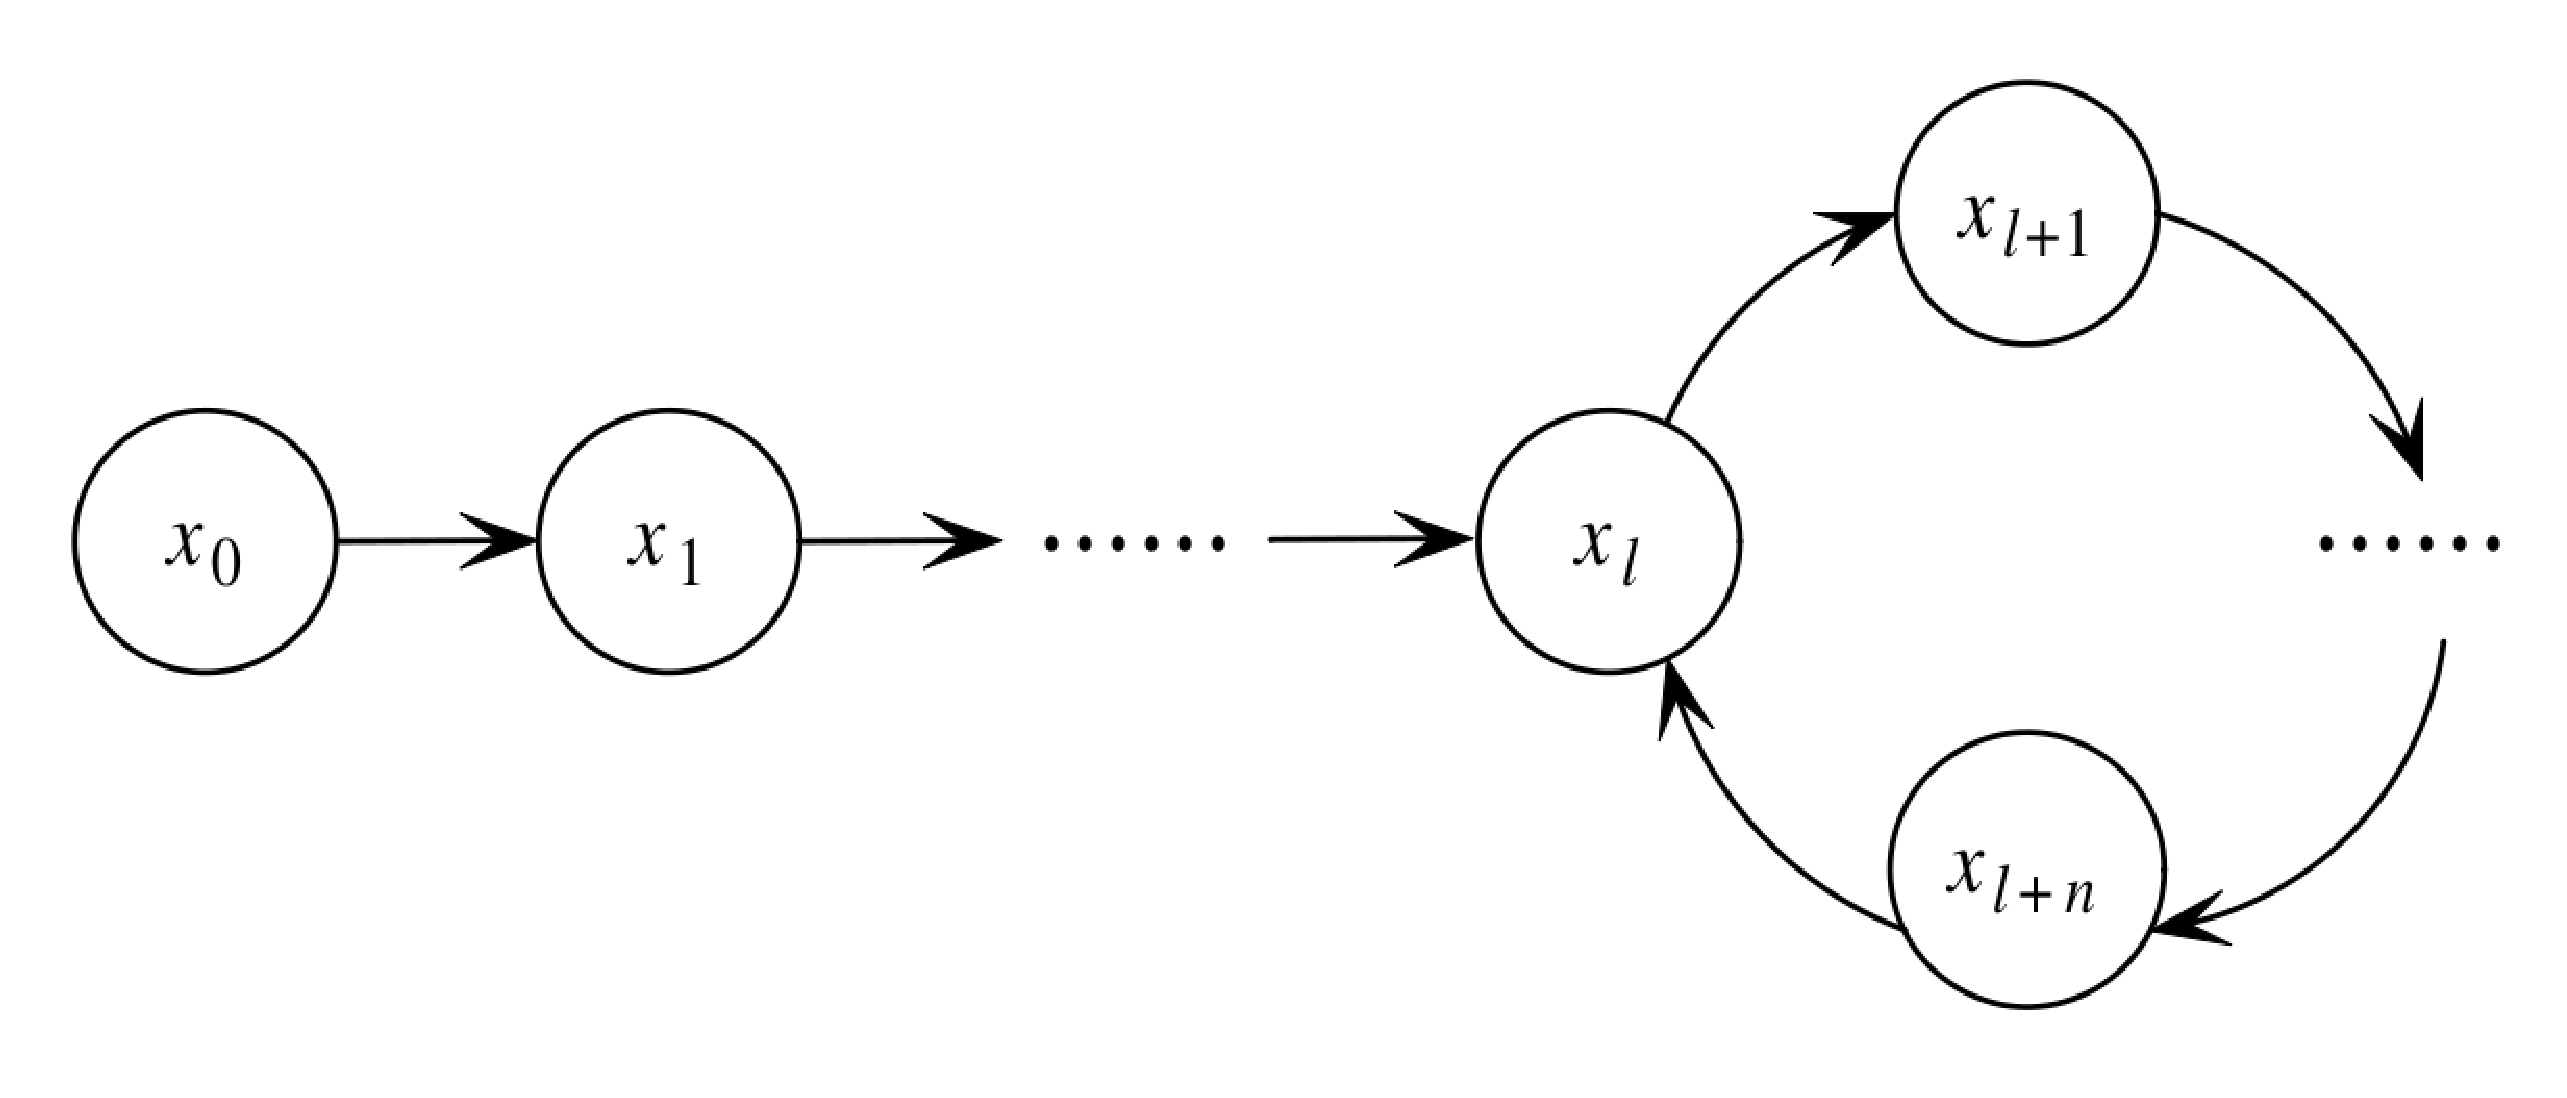
\includegraphics[scale=0.20]{images/pseudo_orbit.eps}
\caption{A pseudo orbit of a digital chaotic system}
\label{A pseudo orbit of a digital chaotic system}
\end{figure}


\begin{definition}%\cite{bahi102008}
A sequence $x = (x^{ 1} , ..., x^{n} )$ is said to be cyclic if a subset of successive terms is repeated from a given rank, until the end of $x$.
\end{definition}

This generator based on discrete chaotic iterations generated by two pseudorandom sequences ($m$ and $w$) has a long cycle length. If the cycle period of $m$ and $w$ are respectivelly $n_{m}$ and $n_{w}$, then in an ideal situation, the cycle period of the novel sequence is $n_{m} \times n_{w}\times 2$ (because $\bar{\bar{x}}=x$). Table \ref{The ideal cycle period} gives the ideal cycle period of various generators.

\begin{itemize}
\item $m$ ($n_{m}=2$): 12121212121212121212121212...

\item $w$ ($n_{w}=4$): 1 23 4 12 3 41 2 34 1 23 4 12 3 41 2 34 1 23 4...

\item $x$ ($n_{x}=2 \times 4 \times 2=16$): 0000(0) 1000(8) 1110(14) 1111(15) 0011(3) 0001(1) 1000(8) 1100(12) 1111(15) 0111(7) 0001(1) 0000(0) 1100(12) 1110(14) 0111(7) 0011(3) 0000(0) 1000(8) 1110(14) 1111(15) 0011(3) 0001(1) 1000(8) 1100(12) 1111(15) 0111(7) 0001(1) 0000(0) 1100(12) 1110(14) 0111(7) 0011(3)...

\end{itemize}


\begin{table}
\renewcommand{\arraystretch}{1.3}
\caption{Ideal cycle period}
\label{The ideal cycle period}
\centering
% \begin{tiny}
\begin{tabular}{|c|c|c|}\toprule\hline
\multicolumn{2}{|c|}{\textbf{PRNG}}&\textbf{Ideal cycle period}\\\hline
\multicolumn{2}{|c|}{\textbf{Logistic map}}& $\infty$\\\hline
\multicolumn{2}{|c|}{\textbf{XORshift}}&$2^{32}-1$ \\\hline
\multicolumn{2}{|c|}{\textbf{ISAAC}}& $2^{8295}$\\\hline
\multirow{4}*{\textbf{Old CI algorithms}}&\textbf{Logistic map 1+Logistic map 2}&$\infty$\\\cline{2-3}
&\textbf{XORshift+XORshift}&$2^{65}$\\\cline{2-3}
&\textbf{XORshift+ISAAC}&$2^{8328}$\\\cline{2-3}
&\textbf{ISAAC+ISAAC}&$2^{16591}$\\\hline
\bottomrule
\end{tabular}
% \end{tiny}
\end{table}


\section{New CI algorithms and examples}
\subsection{Presentation}
The CI generator (generator based on chaotic iterations) is designed by the following process. First of all, some chaotic iterations have to be done to generate a sequence $\left(x^n\right)_{n\in\mathds{N}} \in \left(\mathds{B}^\mathsf{N}\right)^\mathds{N}$ ($\mathsf{N} \in \mathds{N}^*, \mathsf{N} \geqslant 2$, $N$ is not necessarily equal to 32) of boolean vectors, which are the successive states of the iterated system. Some of these vectors will be randomly extracted and our pseudo-random bit flow will be constituted by their components. Such chaotic iterations are realized as follows. Initial state $x^0 \in \mathds{B}^\mathsf{N}$ is a boolean vector taken as a seed (see Section~\ref{algo seed}) and chaotic strategy $\left(S^n\right)_{n\in\mathds{N}}\in \llbracket 1, \mathsf{N} \rrbracket^\mathds{N}$ is
an irregular decimation of a random number sequence (Section~\ref{Chaotic strategy}). The iterate function $f$ is
the vectorial boolean negation:
$$f_0:(x_1,...,x_\mathsf{N}) \in \mathds{B}^\mathsf{N} \longmapsto (\overline{x_1},...,\overline{x_\mathsf{N}}) \in \mathds{B}^\mathsf{N}.$$
At each iteration, only the $S^i$-th component of state $x^n$ is updated, as follows: $x_i^n = x_i^{n-1}$ if $i \neq S^i$, else $x_i^n = \overline{x_i^{n-1}}$.
Finally, some $x^n$ are selected
by a sequence $m^n$ as the pseudo-random bit sequence of our generator.
$(m^n)_{n \in \mathds{N}} \in \mathcal{M}^\mathds{N}$ is computed from a PRNG, such as XORshift sequence $(y^n)_{n \in \mathds{N}} \in \llbracket 0, 2^{32}-1 \rrbracket$ (see Section~\ref{algo m}). So, the
generator returns the following values:\newline
\begin{small}
Bits:$$x_1^{m_0}x_2^{m_0}x_3^{m_0}\hdots x_\mathsf{N}^{m_0}x_1^{m_0+m_1}x_2^{m_0+m_1}\hdots x_\mathsf{N}^{m_0+m_1} x_1^{m_0+m_1+m_2}\hdots$$
or States:$$x^{m_0}x^{m_0+m_1}x^{m_0+m_1+m_2}\hdots$$
\end{small}


\subsection{The seed}
\label{algo seed}
The unpredictability of random sequences is established using
a random seed that is obtained by a physical source like timings of keystrokes.
Without the seed, the attacker must not be able to make any predictions about
the output bits, even when all details of the generator are known~\cite{Turan2008}.

The initial state of the system $x^0$ and the first term $y^0$ of the input PRNG are seeded either by
the current time in seconds since the Epoch, or by a number that the user inputs.
Different ways are possible. For example, let us denote by $t$ the decimal part of the current
time. So $x^0$ can be $t \text{ (mod $2^N$)}$ written in binary digits and $y^0 = t$.

\subsection{Sequence $m$ of returned states}
\label{algo m}
The output of the sequence $(y^n)$ is uniform in $\llbracket 0, 2^{32}-1 \rrbracket$. However, we do not want the output of $(m^n)$ to be uniform in $\llbracket 0, N \rrbracket$, because in this case, the returns of our generator will not be uniform in $\llbracket 0, 2^{N}-1 \rrbracket$, as it is illustrated in the following example. Let us suppose that $x^0=(0,0,0)$. Then $m^0 \in \llbracket 0, 3 \rrbracket$.
\begin{itemize}
\item If $m^0=0$, then no bit will change between the first and the second output of our new CI PRNG. Thus $x^1 = (0,0,0)$.
\item If $m^0=1$, then exactly one bit will change, which leads to three possible values for $x^1$, namely $(1,0,0)$, $(0,1,0)$, and $(0,0,1)$.
\item \emph{etc.}
\end{itemize}
As each value in $\llbracket 0, 2^3-1 \rrbracket$ must be returned with the same probability, then the values $(0,0,0)$, $(1,0,0)$, $(0,1,0)$, and $(0,0,1)$ must occur for $x^1$ with the same probability. Finally we see that, in this example, $m^0=1$ must be three times probable as $m^0=0$.
This leads to the following general definition for the probability of $m=i$:
\begin{equation}
P(m^n=i)=\frac{C^i_N}{2^N}
\end{equation}

Then, here is an example for the $(m^n)$ sequence with a selector function $g_1$
\begin{equation}
\label{Formula}
m^n = g_1(y^n)=
\left\{
\begin{array}{l}
0 \text{ if }0 \leqslant\frac{y^n}{2^{32}}<\frac{C^0_N}{2^N},\\
1 \text{ if }\frac{C^0_N}{2^N} \leqslant\frac{y^n}{2^{32}}<\sum_{i=0}^1\frac{C^i_N}{2^N},\\
2 \text{ if }\sum_{i=0}^1\frac{C^i_N}{2^N} \leqslant\frac{y^n}{2^{32}}<\sum_{i=0}^2\frac{C^i_N}{2^N},\\
\vdots~~~~~ ~~\vdots~~~ ~~~~\\
N \text{ if }\sum_{i=0}^{N-1}\frac{C^i_N}{2^N} \leqslant\frac{y^n}{2^{32}}<1.\\
\end{array}
\right.
\end{equation}

Let us notice, to conclude this subsection, that our new CI PRNG can use any reasonable function as selector. In this paper, $g_1()$ and $g_2()$ are adopted for demonstration purposes, where:
\begin{equation}
m^n = g_2(y^n)=
\left\{
\begin{array}{l}
N \text{ if }0 \leqslant\frac{y^n}{2^{32}}<\frac{C^0_N}{2^N},\\
N-1 \text{ if }\frac{C^0_N}{2^N} \leqslant\frac{y^n}{2^{32}}<\sum_{i=0}^1\frac{C^i_N}{2^N},\\
N-2 \text{ if }\sum_{i=0}^1\frac{C^i_N}{2^N} \leqslant\frac{y^n}{2^{32}}<\sum_{i=0}^2\frac{C^i_N}{2^N},\\
\vdots~~~~~ ~~\vdots~~~ ~~~~\\
0 \text{ if }\sum_{i=0}^{N-1}\frac{C^i_N}{2^N} \leqslant\frac{y^n}{2^{32}}<1.\\
\end{array}
\right.
\end{equation}

In this thesis, $g_1()$ is the selector function unless noted otherwise. And we will show later that both of $g_1()$ and $g_2()$ can pass all of the performed tests. 

%
%This definition has been chosen for the following reason:
%
%The probability $P$ of occurrences of any integer taken in $ \llbracket 0;\mathsf{2^N}-1 \rrbracket$ is $\frac{1}{2^N}$. A string of $N$ binary digits is used to represent this integer; changing $m$ bits of this string will lead to $C_N^m$ different integers.
%
%
%$m^n$ indicates the changing bits between two adjacent output values.
%
%
%If the CI generator generate numbers, each approximately uniformly selected from the set
%$\llbracket 0;\mathsf{2^N}-1 \rrbracket$, the probability
%distribution $P_m$ of $m$ from the XORshift is equal to $\frac{C_N^m}{2^N}$.
%


%$y^0 \in \llbracket 0;2^{32}-1 \rrbracket$ be an integer deduced as a seed too (see Section \ref{algo seed}).
% As shown in Figure~\ref{}, It means that the velue of y_{n+1} can be selected as any values.
% Color histogram. In order to appear random, the color histograms of the encrypted image should be uniform
% distributed in all three color components (RGB). Figs. 6 and 7 show the histograms of RGB colors for the
% original (Fig. 5(a)) and the encrypted images (Fig. 5(b)), respectively. It can be observed that a flat color his-
% togram is resulted from the encrypted image using our scheme. Its uniformity is further justified by the chi-
% square test [14]
In order to evaluate our proposed method and compare its statistical properties with various other methods, the density histogram and intensity map of adjacent output have been computed. The length of $x$ is $N = 4$ bits, and the initial conditions and control
parameters are the same. A large number of
sampled values are simulated ($10^6$ samples). 
%As shown in Figure~\ref{Histogram and intensity map}, it means that the number of adjacent output exists within the sequence. 
Figure~\ref{Histogram1} and Figure~\ref{Histogram2} shows the intensity map for $m^n=g_1(y^n)$ and $m^n=g_2(y^n)$.
In order to appear random, the histogram should be uniformly distributed in all areas. 
It can be observed that uniform histograms and flat color intensity maps are obtained when using our schemes. 
Another illustration of this fact is given by Figure~\ref{Histogram3}, whereas its uniformity is further justified by the tests presented in Section \ref{Results of NISTfor new CI}.
% and for $m^n=y^n~mod~N$ () respectively.  


\begin{figure}[!t]
\centering
\subfigure [The histogram of adjacent output distribution $m^n = g_1(y^n)$]{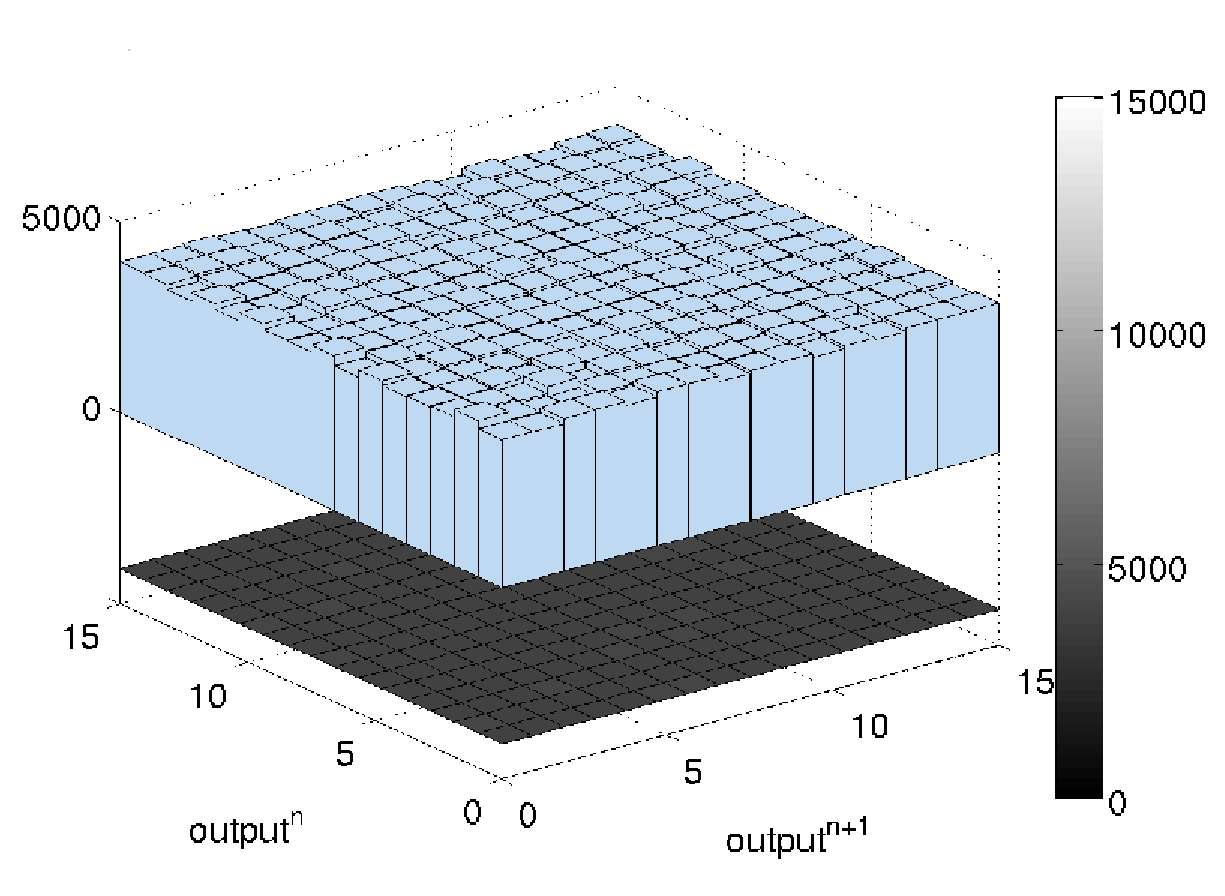
\includegraphics[scale=0.4]{images/f(y).eps}
\label{Histogram1}} \hspace{0.4cm}
\subfigure [The histogram of adjacent output distribution $m^n = g_2(y^n)$]{\includegraphics[scale=0.3]{images/f2(y).eps}
\label{Histogram2}} \hspace{0.4cm}
\subfigure [The histogram of adjacent output distribution $m^n = y^n ~ mod ~ 4$]{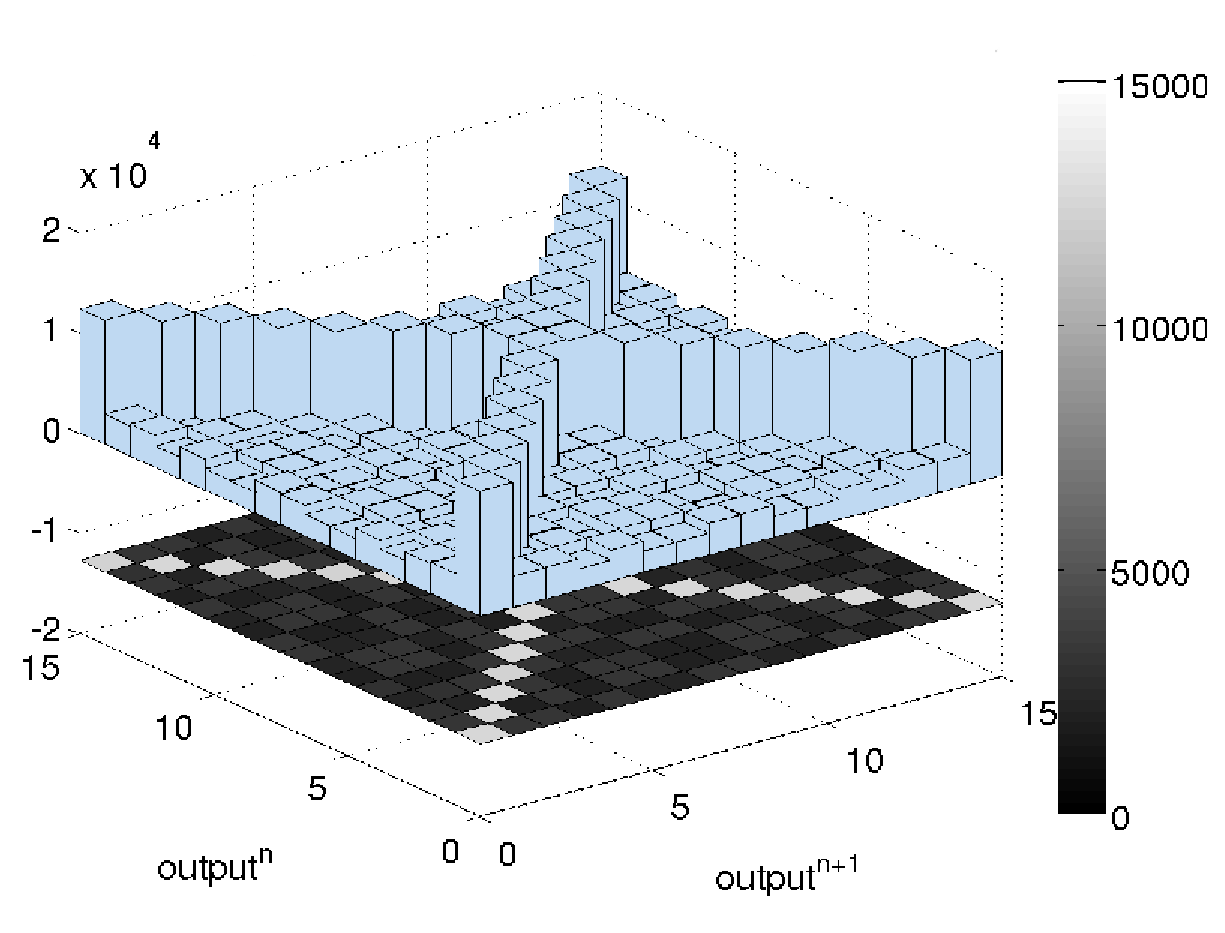
\includegraphics[scale=0.4]{images/y.eps}%
\label{Histogram3}} \hspace{0.4cm}
\caption{Histogram and intensity maps}
\label{Histogram and intensity map1}
\end{figure}


\subsection{Chaotic strategy}
\label{Chaotic strategy}
The chaotic strategy $(S^k) \in \llbracket 1, N \rrbracket^\mathds{N}$ is generated from a second XORshift sequence $(b^k) \in \llbracket 1, N \rrbracket^\mathds{N}$. The only difference between the sequences $S$ and $b$ is that some terms of $b$ are discarded, in such a way that $\forall k \in \mathds{N}, (S^{M^k}, S^{M^k+1}, \hdots, S^{M^{k+1}-1})$ does not contain any given integer twice, where $M^k = \sum_{i=0}^k m^i$. Therefore, no bit will change more than once between two successive outputs of our PRNG, increasing the speed of the former generator by doing so. $S$ is said to be ``an irregular decimation'' of $b$. This decimation can be obtained by the following process.

Let $(d^1,d^2,\dots,d^N)\in \{0,1\}^N$ be a mark sequence, such that whenever $\sum_{i=1}^N d^i = m^k$,
then $\forall i, d_i=0$ ($\forall k$, the sequence is reset when $d$ contains $m^k$ times the number 1). This mark sequence will control the XORshift sequence $b$ as follows:
\begin{itemize}
\item if $d^{b^j} \neq 1$, then $S^k=b^j$, $d^{b^j} = 1$, and $k = k+1$,
\item if $d^{b^j}=1$, then $b^j$ is discarded.
\end{itemize}
For example, if $b = 142\underline{2}334 1421\underline{1}\underline{2}\underline{2}34...$ and $m = 4341...$, then $S=1423~341~4123~4...$ However, if we do not use the mark sequence, then one position may change more than once and the balance property will not be checked, due to the fact that $\bar{\bar{x}}=x$. As an example, for $b$ and $m$ as in the previous example, $S=1422~334~1421~1...$ and $S=14~4~42~1...$ lead to the same output (because switching the same bit twice leads to the same state).

 
To check the balance property, a set of 500
sequences are generated with and without decimation, each
sequence containing $10^6$ bits. Figure~\ref{nmark} shows the
percentages of differences between zeros and ones, and presents a better balance property for the sequences with decimation. This claim will be verified in the tests section (Section \ref{Results of NISTfor new CI}). 


Another example is given in Table~\ref{table application example}, in which $r$ means ``reset'' and the integers which are underlined in sequence $b$ are discarded.
%A simple example illustrates the behavior of this structure.\\
%$m$ : 0,~~~~~~~~~~~~~~~~~~~~~~~~~~~~~~~~~~~~~~~~~~~~~~~~~~~~~~~~~~~4,~~~~~~~~~~~~~~~~~~~~~~~~~~~~~2,\\
%$d$ : r(1,0,0,0),(1,0,0,1),(1,1,0,1),(1,1,1,1),r(0,0,1,0),(0,0,1,1),r \\
%$b$ : ~~~ 1,~~~~~~~~~~~ 4,~~~~~~~~~~~~ 2,~~~~ \underline{2},~~~~ 3,~~~~~~~~~~~~~~3,~~~~~~~~~~~~~ 4,~~~~~~~~~~~~~~~~\\
%$S$ : ~~~1,~~~~~~~~~~~ 4,~~~~~~~~~~~~ 2,~~~~~~~~~~~~ 3,~~~~~~~~~~~~~~3,~~~~~~~~~~~~~ 4,~~~~~~~~~~~~~~~~
%
%Here r means reset, the underlined numbers in the sequence $b_j$ are discarded. In brief, the
%sequence $S$ is an irregular decimation of $b$ by the mark sequence.






\begin{figure}
\centering
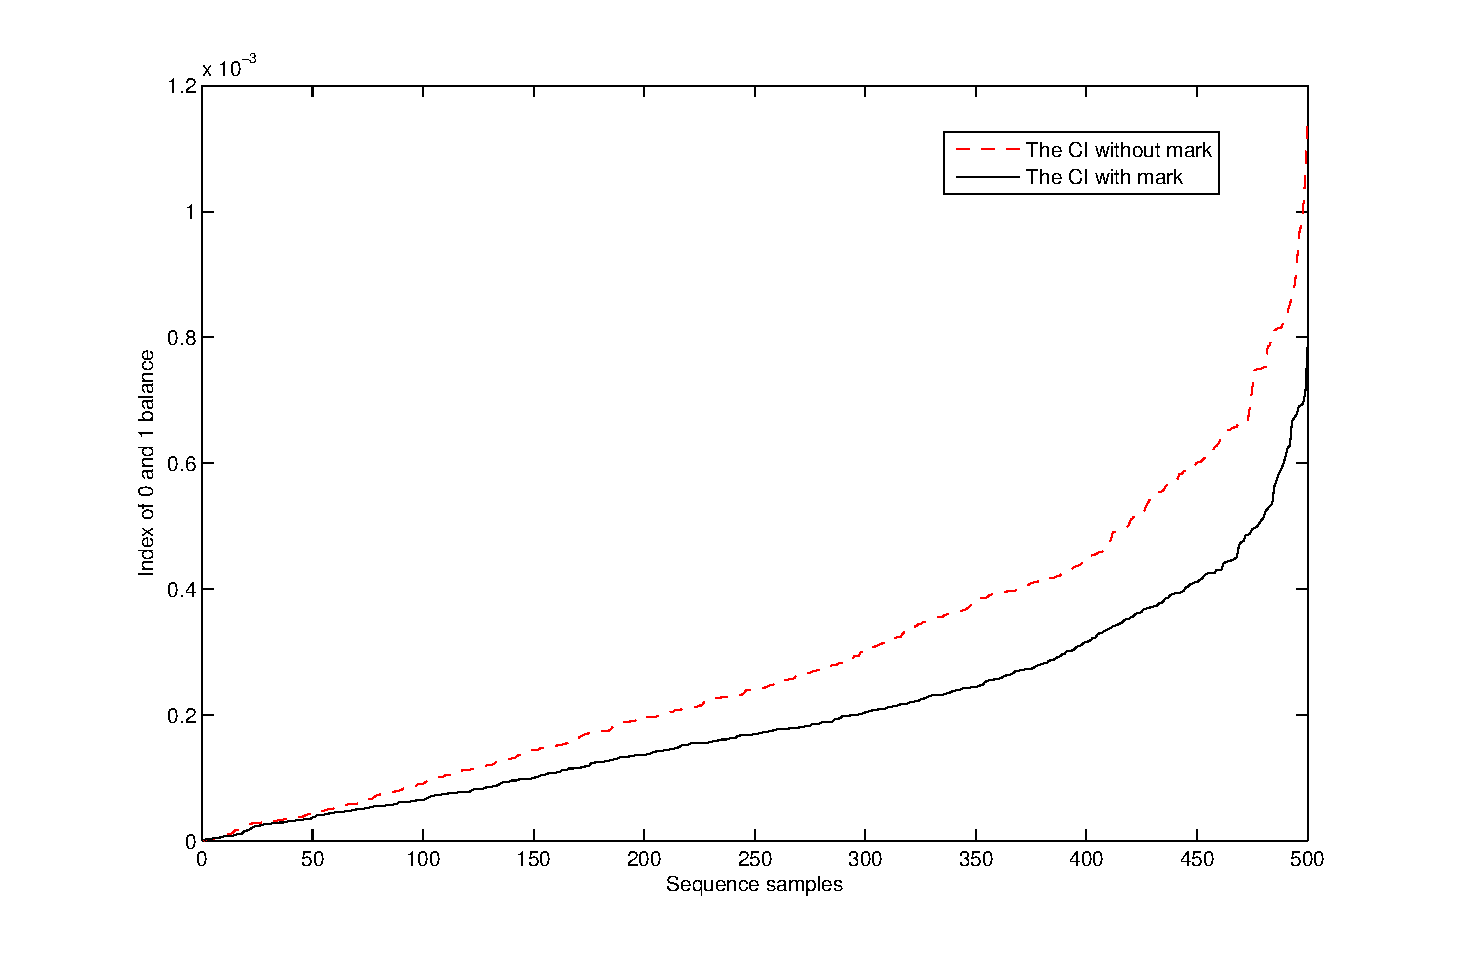
\includegraphics[width=3.85in]{images/nmark.eps}
\DeclareGraphicsExtensions.
\caption{Balance property}
\label{nmark}
\end{figure}

\subsection{New CI(XORshift, XORshift) Algorithm}

The basic design procedure of the novel generator is summed up in Algorithm~\ref{Chaotic iteration1}.
The internal state is $x$, the output state is $r$. $a$ and $b$ are those computed by the two input
PRNGs. The value $g_1(a)$ is an integer, defined as in Equation~\ref{Formula}. Lastly, $\mathsf{N}$ is a constant defined by the user.
\begin{algorithm}
\textbf{Input:} the internal state $x$ ($\mathsf{N}$ bits)\\
\textbf{Output:} a state $r$ of $\mathsf{N}$ bits
\begin{algorithmic}[1]
\FOR{$i=0,\dots,N$}
{
\STATE$d_i\leftarrow{0}$\;
}
\ENDFOR
\STATE$a\leftarrow{PRNG1()}$\;
\STATE$m\leftarrow{f(a)}$\;
\STATE$k\leftarrow{m}$\;
\WHILE{$i=0,\dots,k$}

\STATE$b\leftarrow{PRNG2()~mod~\mathsf{N}}$\;
\STATE$S\leftarrow{b}$\;
    \IF{$d_S=0$}
    {
\STATE      $x_S\leftarrow{ \overline{x_S}}$\;
\STATE      $d_S\leftarrow{1}$\;
    
    }
    \ELSIF{$d_S=1$}
    {
\STATE      $k\leftarrow{ k+1}$\;
    }\ENDIF
\ENDWHILE
$r\leftarrow{x}$\;
return $r$\;
\medskip
\caption{An arbitrary round of the new CI generator}
\label{Chaotic iteration1}
\end{algorithmic}
\end{algorithm}

% 
% \begin{algorithm}
% \SetAlgoLined
% \KwIn{the internal state $x$ ($\mathsf{N}$ bits)}
% \KwOut{a state $r$ of $\mathsf{N}$ bits}
% \For{$i=0,\dots,N$}
% {
% $d_i\leftarrow{0}$\;
% }
% $a\leftarrow{XORshift1()}$\;
% $m\leftarrow{g_1(a)}$\;
% $k\leftarrow{m}$\;
% \For{$i=0,\dots,k$}
% {
% $b\leftarrow{XORshift2()~mod~\mathsf{N}}$\;
% $S\leftarrow{b}$\;
% \If{$d_S=0$}
% {
% $x_S\leftarrow{ \overline{x_S}}$\;
% $d_S\leftarrow{1}$\;
% }
% \ElseIf{$d_S=1$}
% {
% $k\leftarrow{ k+1}$\;
% }
% }
% $r\leftarrow{x}$\;
% return $r$\;
% \medskip
% \caption{An arbitrary round of the new CI(XORshift,XORshift) generator}
% \label{Chaotic iteration1}
% \end{algorithm}

As a comparison, the basic design procedure of the old generator is recalled in Algorithm~\ref{Chaotic iteration2} ($a$ and $b$ are computed by two input PRNGs, $\mathsf{N}$ and $c\geqslant 3\mathsf{N}$ are constants defined by the user). See Subsection~\ref{Old CI algorithms and examples} for further information.

% \begin{algorithm}
% \SetAlgoLined
% \KwIn{the internal state $x$ ($\mathsf{N}$ bits)}
% \KwOut{a state $r$ of $\mathsf{N}$ bits}
% $a\leftarrow{Logistic map1()}$\;
% \If{$a>0.5$}
% {
% $d\leftarrow 1$
% }
% \Else
% {
% $d\leftarrow 0$
% }
% 
% $m\leftarrow{d+c}$\;
% \For{$i=0,\dots,m$}
% {
% $b\leftarrow{Logistic map2()}$\;
% $S\leftarrow{100000b~mod~\mathsf{N}}$\;
% $x_S\leftarrow{ \overline{x_S}}$\;
% }
% $r\leftarrow{x}$\;
% return $r$\;
% \medskip
% \caption{An arbitrary round of the old CI PRNG}
% \label{Chaotic iteration2}
% \end{algorithm}
\begin{algorithm}
\textbf{Input:} the internal state $x$ (an array of $\mathsf{N}$ 1-bit words)\\
\textbf{Output:} an array $r$ of $\mathsf{N}$ 1-bit words
\begin{algorithmic}[1]

\STATE$a\leftarrow{PRNG1()}$;
\STATE$m\leftarrow{a~mod~2+c}$;
\WHILE{$i=0,\dots,m$}
\STATE$b\leftarrow{PRNG2()}$;
\STATE$S\leftarrow{b~mod~\mathsf{N}}$;
\STATE$x_S\leftarrow{ \overline{x_S}}$;
\ENDWHILE
\STATE$r\leftarrow{x}$;
\STATE return $r$;
\medskip
\caption{An arbitrary round of the old CI generator}
\label{Chaotic iteration2}
\end{algorithmic}
\end{algorithm}


\subsection{Illustrative Example}

In this example, $\mathsf{N} = 4$ is chosen for easy understanding and the input PRNG is XORshift PRNG.
As stated before, the initial state of the system $x^0$ can be seeded by the decimal part $t$ of the current time.
For example, if the current time in seconds since the Epoch is 1237632934.484088,
so $t = 484088$, then $x^0 = t \text{ ($mod$ 16)}$ in binary digits, \emph{i.e.}, $x^0 = ( 0, 1, 0, 0)$.

To compute $m$ sequence, Equation~\ref{Formula} can be adapted to this example as follows:
\begin{equation}
\label{m1 fuction}
m^n=g_1(y^n)=
\left\{
\begin{array}{llccccc}
0 & \text{ if }&0 &\leqslant&\frac{y^n}{2^{32}}&<&\frac{1}{16},\\
1 & \text{ if }&\frac{1}{16} &\leqslant&\frac{y^n}{2^{32}}&<&\frac{5}{16} ,\\
2 & \text{ if }&\frac{5}{16} &\leqslant&\frac{y^n}{2^{32}}&<&\frac{11}{16},\\
3 & \text{ if }&\frac{11}{16} &\leqslant&\frac{y^n}{2^{32}}&<&\frac{15}{16},\\
4 & \text{ if }&\frac{15}{16} &\leqslant&\frac{y^n}{2^{32}}&<&1,\\
\end{array}
\right.
\end{equation}

\noindent where $y$ is generated by XORshift seeded with the current time. We can see that the probabilities of occurrences of $m=0$, $m=1$, $m=2$, $m=3$, $m=4$, are $\frac{1}{16}$, $\frac{4}{16}$, $\frac{6}{16}$, $\frac{4}{16}$, $\frac{1}{16}$, respectively. This $m$ determines what will be the next output $x$. For instance,
\begin{itemize}
\item If $m=0$, the following $x$ will be $( 0, 1, 0, 0)$.
\item If $m=1$, the following $x$ can be $( 1, 1, 0, 0)$, $( 0, 0, 0, 0)$, $( 0, 1, 1, 0)$, or $( 0, 1, 0, 1)$.
\item If $m=2$, the following $x$ can be $( 1, 0, 0, 0)$, $( 1, 1, 1, 0)$, $( 1, 1, 0, 1)$, $( 0, 0, 1, 0)$, $( 0, 0, 0, 1)$, or $( 0, 1, 1, 1)$.
\item If $m=3$, the following $x$ can be $( 0, 0, 1, 1)$, $( 1, 1, 1, 1)$, $( 1, 0, 0, 1)$, or $( 1, 0, 1, 0)$.
\item If $m=4$, the following $x$ will be $( 1, 0, 1, 1)$.
\end{itemize}

In this simulation, $m = 0, 4, 2, 2, 3, 4, 1, 1, 2, 3, 0, 1, 4,...$ Additionally, $b$ is computed with a XORshift generator too, but with another seed. We have found $b = 1, 4, 2, 2, 3, 3, 4, 1, 1, 4, 3, 2, 1,...$

Chaotic iterations are made with initial state $x^0$, vectorial logical negation $f_0$, and
strategy $S$. The result is presented in Table~\ref{table application example}. Let us recall that sequence $m$ gives the states $x^n$ to return, which are here $x^0, x^{0+4}, x^{0+4+2}, \hdots$ So, in this example, the output of the generator is: 10100111101111110011... or 4,4,11,8,1...




\begin{table*}[!t]
%\renewcommand{\arraystretch}{1.3}
\centering
\begin{tabular}{|c|c@{}c|c@{}c@{}c@{}c@{}c@{}c|c@{}c@{}c|c@{}c@{}c@{}c|}
\hline
$m$ &0 & &4 & & & & & &2& &&2&&  &  \\ \hline
$k$ &0 & &4 & & &$+1$ & & &2& &&2&$+1$&  &  \\ \hline
$b$  &  & &1 &4&2&\underline{2}       &3& &3&4&&1&\underline{1}      &4&\\ \hline
$d$  &r  & &r~$\left(\begin{array}{c}1\\0\\0\\0\end{array}\right)$ & $\left(\begin{array}{c}1\\0\\0\\1\end{array}\right)$ & $\left(\begin{array}{c}1\\1\\0\\1\end{array}\right)$ & & $\left(\begin{array}{c}1\\1\\1\\1\end{array}\right)$ && r~$\left(\begin{array}{c}0\\0\\1\\0\end{array}\right)$ &$\left(\begin{array}{c}0\\0\\1\\1\end{array}\right)$ &&r~$\left(\begin{array}{c}1\\0\\0\\0\end{array}\right)$ & &$\left(\begin{array}{c}1\\0\\0\\1\end{array}\right)$  &  \\ \hline
$S$  &  & &1 &4&2&        &3& &3&4&&1& &4 &  \\ \hline
$x^{0}$ &  &$x^{0}$ & & &  
&  & &$x^{4}$ & & &   
$x^{6}$& & &&$x^{8}$  \\
%1ere ligne
0 & &0 &$\xrightarrow{1} 1$ & &
 & &   &1   & & &
1 &$\xrightarrow{1} 0$ & & & 0\\
%2eme ligne
1 &  &1 &   &   &
$\xrightarrow{2} 0$ & & &0 & & &
0 & &  &&0\\
%3eme ligne
0 & &0 & & &
 & &$\xrightarrow{3} 1$ &1 &$\xrightarrow{3} 0$ & &
0 &   & & &0  \\
% 4eme ligne
0 & &0  & &$\xrightarrow{4} 1$ &
 & & &1 & &$\xrightarrow{4} 0$ &
0 & & &$\xrightarrow{4} 1$&1 \\
\hline
\end{tabular}\\
\vspace{0.5cm}
Binary Output: $x_1^{0}x_2^{0}x_3^{0}x_4^{0}x_1^{4}x_2^{4}x_3^{4}x_4^{4}x_1^{6}x_2^{6}... = 0100101110000001...$\\
Integer Output:
$x^{0},x^{4},x^{6},x^{8}... = 4,11,8,1...$
\caption{Example of New CI(XORshift,XORshift) generation}
\label{table application example}
\end{table*}







% 
% \section{Chaotic iterations as pseudo-random generator}
% \subsection{Presentation}
% 
% The CI generator is designed by the following process \cite{wang2009,wbg10:ip}. 
% 
% Chaotic iterations are done to generate a sequence $\left(x^n\right)_{n\in\mathds{N}} \in \left(\mathds{B}^\mathsf{N}\right)^\mathds{N}$ ($\mathsf{N} \in \mathds{N}^*, \mathsf{N} \geqslant 2$) of boolean vectors, which are the successive states of the iterated system. Some of these vectors are randomly extracted and the pseudo-random bit flow is constituted by their components. These chaotic iterations are realized as follows. 
% 
% Initial state $x^0 \in \mathds{B}^\mathsf{N}$ is a boolean vector taken as a seed (see Section~\ref{algo seed}) and chaotic strategy $\left(S^n\right)_{n\in\mathds{N}}\in \llbracket 1, \mathsf{N} \rrbracket^\mathds{N}$ is defined with a XORshift sequence (Old CI generator \cite{wang2009}) or an irregular decimation of it (New CI generatot \cite{wbg10:ip}), as it is explained in Section~\ref{Chaotic strategy}). Lastly, the iterate function $f$ is the vectorial boolean negation.
% 
% More precisely, at each iteration, only $S^i$-th component of state $x^n$ is updated as follows
% \begin{equation}
% x_i^n = \left\{\begin{array}{ll}x_i^{n-1} & \text{if } i \neq S^i, \\ \\ \overline{x_i^{n-1}} & \text{if } i = S^i. \\\end{array}\right.
% \end{equation}
% Then, let $\mathcal{M}$ be a finite subset of $\mathds{N}^*$. Some $x^n$ are selected by a sequence $m^n$ as the pseudo-random bit sequence of our generator. The sequence $(m^n)_{n \in \mathds{N}} \in \mathcal{M}^\mathds{N}$ is computed from XORshift (or from a decimation of it, in case of the new CI generator). So, the generator returns the following values:
% \begin{itemize}
% \item the components of $x^{m^0}$,
% \item following by the components of $x^{m^0+m^1}$,
% \item following by the components of $x^{m^0+m^1+m^2}$,
% \item \emph{etc.}
% \end{itemize}
% In other words, the generator returns the following bits:\newline
% \begin{small}
% $$x_1^{m_0}x_2^{m_0}x_3^{m_0}\hdots x_\mathsf{N}^{m_0}x_1^{m_0+m_1}x_2^{m_0+m_1}\hdots x_\mathsf{N}^{m_0+m_1} x_1^{m_0+m_1+m_2}x_2^{m_0+m_1+m_2}\hdots$$
% \end{small}
% 
% 
% 
% \subsection{The seed}
% \label{algo seed}
% 
% The initial state of the system $x^0$ and the first term $y^0$ of the XORshift are seeded either by the current time in seconds since the Epoch, or by a number that the user inputs, as it is usually the case for every PRNG.
% 
% \subsection{Sequence $m$ of returned states}
% \label{algo m}
% 
% The output of a sequence $(y^n)$ produced by a XORshift generator is uniform in $\llbracket 0, 2^{32}-1 \rrbracket$. However, we do not want the output of $(m^n)$ to be uniform in $\llbracket 0, N \rrbracket$, because in this case, the returns of our generator will not be uniform in $\llbracket 0, 2^{N}-1 \rrbracket$, as it is illustrated in the following example. Let us suppose that $x^0=(0,0,0)$. Then $m^0 \in \llbracket 0, 3 \rrbracket$.
% \begin{itemize}
% \item If $m^0=0$, then no bit will change between the first and the second output of our PRNG. Thus $x^1 = (0,0,0)$.
% \item If $m^0=1$, then exactly one bit will change, which leads to three possible values for $x^1$, namely $(1,0,0)$, $(0,1,0)$, and $(0,0,1)$.
% \item \emph{etc.}
% \end{itemize}
% As each value in $\llbracket 0, 2^3-1 \rrbracket$ must be returned with the same probability, then the values $(0,0,0)$, $(1,0,0)$, $(0,1,0)$ and $(0,0,1)$ must occur for $x^1$ with the same probability. Finally we see that, in this example, $m^0=1$ must be three times more probable than $m^0=0$.
% This leads to the following general definition for $m$:
% \begin{equation}
% \label{Formula}
% m^n = f(y^n)=
% \left\{
% \begin{array}{l}
% 0 \text{ if }0				\leqslant\frac{y^n}{2^{32}}<\frac{C^0_N}{2^N},\\
% 1 \text{ if }\frac{C^0_N}{2^N}		\leqslant\frac{y^n}{2^{32}}<\sum_{i=0}^1\frac{C^i_N}{2^N},\\
% 2 \text{ if }\sum_{i=0}^1\frac{C^i_N}{2^N}	\leqslant\frac{y^n}{2^{32}}<\sum_{i=0}^2\frac{C^i_N}{2^N},\\
% \vdots~~~~~					~~\vdots~~~		    ~~~~\\
% N \text{ if }\sum_{i=0}^{N-1}\frac{C^i_N}{2^N}	\leqslant\frac{y^n}{2^{32}}<1.\\
% \end{array}
% \right.
% \end{equation}
% %
% %This definition has been chosen for the following reason: 
% %
% %The probability $P$ of occurrences of any integer taken in $ \llbracket 0;\mathsf{2^N}-1 \rrbracket$ is $\frac{1}{2^N}$. A string of $N$ binary digits is used to represent this integer; changing $m$ bits of this string will lead to $C_N^m$ different integers.
% %
% %
% %$m^n$ indicates the changing bits between two adjacent output values.
% %
% %
% %If the CI generator generate numbers, each approximately uniformly selected from the set 
% %$\llbracket 0;\mathsf{2^N}-1 \rrbracket$, the probability 
% %distribution $P_m$ of $m$ from the XORshift is equal to $\frac{C_N^m}{2^N}$.
% %
% 
% 
% %$y^0 \in \llbracket 0;2^{32}-1 \rrbracket$ be an integer deduced as a seed too (see Section \ref{algo seed}).
% 
% 
% \subsection{Chaotic strategy}
% \label{Chaotic strategy}
% 
% The chaotic strategy $(S^k) \in \llbracket 1, N \rrbracket^\mathds{N}$ is generated from a second XORshift sequence $(b^k) \in \llbracket 1, N \rrbracket^\mathds{N}$. In the Old CI generator, $S=b$. In the New CI generator, the sole difference between the sequences $S$ and $b$ is that some terms of $b$ are discarded, in such a way that: $\forall k \in \mathds{N}, (S^{M^k}, S^{M^k+1}, \hdots, S^{M^{k+1}-1})$ does not contain a same integer twice, where $M^k = \sum_{i=0}^k m^i$. Therefore, in New CI generator, no bit will change more than once between two successive outputs of our PRNG, increasing the speed of the former generator by doing so. $S$ is said to be ``an irregular decimation'' of $b$. This decimation can be obtained by the following process.
% 
% Let $(d^1,d^2,\dots,d^N)\in \{0,1\}^N$ be a mark sequence, such that whenever $\sum_{i=1}^N d^i = m^k$, 
% then $\forall i, d_i=0$ ($\forall k$, the sequence is reset when $d$ contains $m^k$ times the number 1). This mark sequence will control the XORshift sequence $b$ as follows:
% \begin{itemize}
% \item if $d^{b^j} \neq 1$, then $S^k=b^j$, $d^{b^j} = 1$, and $k = k+1$,
% \item if $d^{b^j}=1$, then $b^j$ is discarded.
% \end{itemize}
% For example, if $b = 142\underline{2}334 142\underline{1}\underline{1}\underline{2}\underline{2}34...$ and $m = 4241...$, then $S=1423~34~1423~4...$ Another example is given in Table~\ref{table application example}, in which $r$ means ``reset'' and the integers which are underlined in sequence $b$ are discarded.
% 
% 
% 
% %\subsection{Old CI pseudo-random sequence}
% %\label{The generation of pseudo-random sequence}
% 
% %The design of the PRNG based on discrete chaotic iterations is proposed in this section, while its performance is evaluated in the next sections.
% %The old CI generator is designed by the following process.
% %Let $\mathsf{N} \in \mathds{N}^*, \mathsf{N} \geqslant 2$. Some chaotic iterations are done, which generate a sequence $\left(x^n\right)_{n\in\mathds{N}} \in \left(\mathds{B}^\mathsf{N}\right)^\mathds{N}$ of boolean vectors: the successive states of the iterated system. Some of these vectors are chaotically extracted and their components constitute our pseudo-random bit flow.
% %Chaotic iterations are realized as follows: initial state\linebreak $x^0 \in \mathds{B}^\mathsf{N}$ is a boolean vector taken as a seed and chaotic strategy $\left(S^n\right)_{n\in\mathds{N}}\in \llbracket 1, \mathsf{N} \rrbracket^\mathds{N}$ is constructed with XORshift. Lastly, iterate function $f$ is the vectorial boolean negation
% %$$f_0:(x_1,...,x_\mathsf{N}) \in \mathds{B}^\mathsf{N} \longmapsto (\overline{x_1},...,\overline{x_\mathsf{N}}) \in \mathds{B}^\mathsf{N}.$$
% 
% 
% 
% 
% 
% 
% \section{CI(XORshift, XORshift) algorithms and examples}
% 
% \subsection{Algorithms}
% 
% The basic design procedure of the old generator is recalled in Algorithm~\ref{Chaotic iteration2} ($a$ and $b$ are computed by XORshift generators, $\mathsf{N}$ and $c\geqslant 3\mathsf{N}$ are constants defined by the user). 
% Algorithm~\ref{Chaotic iteration1} summarizes the basic design procedure of the new generator. The internal state is $x$, the output state is $r$. $a$ and $b$ are those computed by the two XORshift generators. The value $f(a)$ is an integer, defined as in Equation~\ref{Formula}. Lastly, $\mathsf{N}$ is a constant defined by the user.
% 
% 
% \begin{algorithm}
% \textbf{Input:} the internal state $x$ (an array of $\mathsf{N}$ 1-bit words)\\
% \textbf{Output:} an array $r$ of $\mathsf{N}$ 1-bit words
% \begin{algorithmic}[1]
% 
% \STATE$a\leftarrow{XORshift1()}$;
% \STATE$m\leftarrow{a~mod~2+c}$;
% \WHILE{$i=0,\dots,m$}
% \STATE$b\leftarrow{XORshift2()}$;
% \STATE$S\leftarrow{b~mod~\mathsf{N}}$;
% \STATE$x_S\leftarrow{ \overline{x_S}}$;
% \ENDWHILE
% \STATE$r\leftarrow{x}$;
% \STATE return $r$;
% \medskip
% \caption{An arbitrary round of the old CI(XORshift,XORshift) generator}
% \label{Chaotic iteration2}
% \end{algorithmic}
% \end{algorithm}
% 
% 
% \subsection{Old CI(XORshift,XORshift) example}
% 
% 
% 
% In this example, $\mathsf{N} = 5$ and $\mathcal{M} = \{\text{4,5}\}$ are adopted for easy understanding.
% The initial state of the system $x^0$ can be seeded by the decimal part of the current time. For example, the current time in seconds since the Epoch is 1237632934.484084, so $t = 484084$. $x^0 = t \text{ (mod 32)}$ in binary digits, then $x^0 = (1, 0, 1, 0, 0)$. $m$ and $S$ can now be computed from two XORshift PRNGs:
% 
% $m$ = 4, 5, 4, 4, 4, 4, 5, 5, 5, 5, 4, 5, 4,...
% 
% $S$ = 2, 4, 2, 2, 5, 1, 1, 5, 5, 3, 2, 3, 3,...
% 
% Chaotic iterations are done with initial state $x^0$, vectorial logical negation $f_0$ and strategy $S$. The result is presented in Table \ref{Table:old CI}. Let us recall that sequence $m$ gives the states $x^n$ to return: $x^4, x^{4+5}, x^{4+5+4}, \hdots$
% 
% 
% \begin{tiny}
% \begin{table}[!t]
% \renewcommand{\arraystretch}{1.3}
% \caption{Application example (Old CI generator)}
% \label{Table:old CI}
% \centering
% \begin{tabular}{c|c@{}c@{}c@{}c@{}c|c@{}c@{}c@{}c@{}c@{}c|c@{}c@{}c@{}c@{}c@{}c}
% \hline\hline
% $m:$ & & & 4 & & & & & 5 & & & & & & 4 & & & \\ \hline
% $S$ & 2 & 4 & 2 & 2 & & 5 & 1 & 1 & 5 & 5 & & 3 & 2 & 3 & 3 & & \\ \hline
% $x^{0}$ & & & & & $x^{4}$ & & & & & & $x^{9}$ & & & & & $x^{13}$ & \\
% %1ere ligne
% 1 & & & & &
% 1 & & $\xrightarrow{1} 0$ & $\xrightarrow{1} 1$ & & &
% 1 & & & & &
% 1 & \\
% %2eme ligne
% 0 & $\xrightarrow{2} 1$ & & $\xrightarrow{2} 0$ & $\xrightarrow{2} 1$ &
% 1 & & & & & &
% 1 & & $\xrightarrow{2} 0$ & & & 0 &\\
% %3eme ligne
% 1 & & & & &
% 1 & & & & & &
% 1 & $\xrightarrow{3} 0$ & & $\xrightarrow{3} 1$ & $\xrightarrow{3} 0$ &
% 0 &\\
% % 4eme ligne
% 0 & & $\xrightarrow{4} 1$ & & &
% 1 & & & & & &
% 1 & & & & &
% 1 &\\
% %5eme ligne
% 0 & & & & &
% 0 & $\xrightarrow{5} 1$ & & & $\xrightarrow{5} 0$ & $\xrightarrow{5} 1$ &
% 1 & & & & &
% 1 &\\
% \hline\hline
% \end{tabular}\\
% \vspace{0.5cm}
% Output: $x_1^{0}x_2^{0}x_3^{0}x_4^{0}x_5^{0}x_1^{4}x_2^{4}x_3^{4}x_4^{4}x_5^{4}x_1^{9}x_2^{9}x_3^{9}x_4^{9}$
% $x_5^{9}x_1^{13}x_2^{13}x_3^{13}x_4^{13}x_5^{13}... = 10100111101111110011...$
% \end{table}
% \end{tiny}
% So, in this example, the output of the generator is: 10100111101111110011...
% 
% 
% 
% \begin{algorithm}
% \textbf{Input:} the internal state $x$ ($\mathsf{N}$ bits)\\
% \textbf{Output:} a state $r$ of $\mathsf{N}$ bits
% \begin{algorithmic}[1]
% \FOR{$i=0,\dots,N$}
% {
% \STATE$d_i\leftarrow{0}$\;
% }
% \ENDFOR
% \STATE$a\leftarrow{XORshift1()}$\;
% \STATE$m\leftarrow{f(a)}$\;
% \STATE$k\leftarrow{m}$\;
% \WHILE{$i=0,\dots,k$}
% 
% \STATE$b\leftarrow{XORshift2()~mod~\mathsf{N}}$\;
% \STATE$S\leftarrow{b}$\;
%     \IF{$d_S=0$}
%     {
% \STATE      $x_S\leftarrow{ \overline{x_S}}$\;
% \STATE      $d_S\leftarrow{1}$\;
%     
%     }
%     \ELSIF{$d_S=1$}
%     {
% \STATE      $k\leftarrow{ k+1}$\;
%     }\ENDIF
% \ENDWHILE
% $r\leftarrow{x}$\;
% return $r$\;
% \medskip
% \caption{An arbitrary round of the new CI(XORshift,XORshift) generator}
% \label{Chaotic iteration1}
% \end{algorithmic}
% \end{algorithm}
% 
% 
% 
% 
% 
% \subsection{New CI(XORshift,XORshift) example}
% 
% In this example, $\mathsf{N} = 4$ is chosen for easy understanding.
% The initial state of the system $x^0$ can be seeded another time by the decimal part $t$ of the current time. 
% For example, if the current time in seconds since the Epoch is 1237632934.484088, 
% so $t = 484088$, then $x^0 = t \text{ (mod 16)}$ in binary digits, \emph{i.e.}, $x^0 = ( 0, 1, 0, 0)$. 
% 
% To compute $m$ sequence, Equation~\ref{Formula} can be adapted to this example as follows:
% \begin{equation}
% \label{m1 fuction}
% m^n=f(y^n)=
% \left\{
% \begin{array}{llccccc}
% 0 & \text{ if }&0				&\leqslant&\frac{y^n}{2^{32}}&<&\frac{1}{16},\\
% 1 & \text{ if }&\frac{1}{16}			&\leqslant&\frac{y^n}{2^{32}}&<&\frac{5}{16} ,\\
% 2 & \text{ if }&\frac{5}{16}			&\leqslant&\frac{y^n}{2^{32}}&<&\frac{11}{16},\\
% 3 & \text{ if }&\frac{11}{16}			&\leqslant&\frac{y^n}{2^{32}}&<&\frac{15}{16},\\
% 4 & \text{ if }&\frac{15}{16}			&\leqslant&\frac{y^n}{2^{32}}&<&1,\\
% \end{array}
% \right.
% \end{equation}
% 
% \noindent where $y$ is generated by XORshift seeded with the current time. We can see that the probabilities of occurrences of $m=0$, $m=1$, $m=2$, $m=3$, $m=4$, are $\frac{1}{16}$, $\frac{4}{16}$, $\frac{6}{16}$, $\frac{4}{16}$, $\frac{1}{16}$, respectively. This $m$ determines what will be the next output $x$. For instance, 
% \begin{itemize}
% \item If $m=0$, the following $x$ will be $( 0, 1, 0, 0)$.
% \item If $m=1$, the following $x$ can be $( 1, 1, 0, 0)$, $( 0, 0, 0, 0)$, $( 0, 1, 1, 0)$, or $( 0, 1, 0, 1)$.
% \item If $m=2$, the following $x$ can be $( 1, 0, 0, 0)$, $( 1, 1, 1, 0)$, $( 1, 1, 0, 1)$, $( 0, 0, 1, 0)$, $( 0, 0, 0, 1)$, or $( 0, 1, 1, 1)$.
% \item If $m=3$, the following $x$ can be $( 0, 0, 1, 1)$, $( 1, 1, 1, 1)$, $( 1, 0, 0, 1)$, or $( 1, 0, 1, 0)$.
% \item If $m=4$, the following $x$ will be $( 1, 0, 1, 1)$.
% \end{itemize}
% 
% In this simulation, $m = 0, 4, 2, 2, 3, 4, 1, 1, 2, 3, 0, 1, 4,...$ Additionally, $b$ is computed with a XORshift generator too, but with another seed. We have found $b = 1, 4, 2, 2, 3, 3, 4, 1, 1, 4, 3, 2, 1,...$
% 
% Chaotic iterations are made with initial state $x^0$, vectorial logical negation $f_0$ and 
% strategy $S$. The result is presented in Table~\ref{table application example}. Let us recall that sequence $m$ gives, after decimation, the states $x^n$ to return, which are here $x^0, x^{0+4}, x^{0+4+2}, \hdots$ So, in this example, the output of the generator is: 0100101110000001... or 4,11,8,1... 
% 
% 
% 
% 
% 
% 
% \begin{table}[!t]
% \label{CI(XORshift, XORshift) algorithm}
% %\renewcommand{\arraystretch}{1.3}
% \centering
% % \begin{tabular}{0.75\textwidth}{|c|cc|cccccc|ccc|cccc|}
% \begin{tabular}{|c|c@{}c|c@{}c@{}c@{}c@{}c@{}c|c@{}c@{}c|c@{}c@{}c@{}c|}
% \hline
% $m$ &0 & &4 & & & & & &2& &&2&&  &  \\ \hline
% $k$ &0 & &4 & & &$+1$ & & &2& &&2&$+1$&  &  \\ \hline
% $b$  &  & &1 &4&2&\underline{2}       &3& &3&4&&1&\underline{1}      &4&\\ \hline
% $d$  &r  & &r~$\left(\begin{array}{c}1\\0\\0\\0\end{array}\right)$ & $\left(\begin{array}{c}1\\0\\0\\1\end{array}\right)$ & $\left(\begin{array}{c}1\\1\\0\\1\end{array}\right)$ & & $\left(\begin{array}{c}1\\1\\1\\1\end{array}\right)$ && r~$\left(\begin{array}{c}0\\0\\1\\0\end{array}\right)$ &$\left(\begin{array}{c}0\\0\\1\\1\end{array}\right)$ &&r~$\left(\begin{array}{c}1\\0\\0\\0\end{array}\right)$ & &$\left(\begin{array}{c}1\\0\\0\\1\end{array}\right)$  &  \\ \hline
% $S$  &  & &1 &4&2&        &3& &3&4&&1& &4 &  \\ \hline
% $x^{0}$ &  &$x^{0}$ & & &  
% &  & &$x^{4}$ & & &   
% $x^{6}$& & &&$x^{8}$  \\
% %1ere ligne
% 0 & &0 &$\xrightarrow{1} 1$ & &
%  & &   &1   & & &
% 1 &$\xrightarrow{1} 0$ & & & 0\\
% %2eme ligne
% 1 &  &1 &   &   &
% $\xrightarrow{2} 0$ & & &0 & & &
% 0 & &  &&0\\
% %3eme ligne
% 0 & &0 & & &
%  & &$\xrightarrow{3} 1$ &1 &$\xrightarrow{3} 0$ & &
% 0 &   & & &0  \\
% % 4eme ligne
% 0 & &0  & &$\xrightarrow{4} 1$ &
%  & & &1 & &$\xrightarrow{4} 0$ &
% 0 & & &$\xrightarrow{4} 1$&1 \\
% \hline
% \end{tabular}\\
% \vspace{0.5cm}
% Binary Output: $x_1^{0}x_2^{0}x_3^{0}x_4^{0}x_1^{4}x_2^{4}x_3^{4}x_4^{4}x_1^{6}x_2^{6}... = 0100101110000001...$\\
% Integer Output:
% $x^{0},x^{4},x^{6},x^{8}... = 4,11,8,1...$
% \caption{Example of New CI(XORshift,XORshift) generation}
% \label{table application example}
% \end{table}





\chapter{Randomness}
\label{Statistical Tests for Randomness}
\minitoc

\section{Some famous statistical tests of random number generators}
\label{Some famous statistical tests of random number generators}

A theoretical proof for the randomness of a generator is impossible to give, therefore statistical inference based on observed sample sequences produced by the generator seems to be the best option. Considering the properties of binary
random sequences, various statistical tests can be designed to evaluate the assertion
that the sequence is generated by a perfectly random source. 
We have performed certain statistical tests for various CI PRNGs we proposed. These tests
include TestU01~\cite{Lecuyer2009}, NIST suite~\cite{ANDREW2008},
Diehard battery of tests~\cite{Marsaglia1996}, and Comparative test parameters. For completeness and for reference, we give
in the following subsection a brief description of each of the
aforementioned tests.



\subsection{NIST statistical test suite}



Among the numerous standard tests for pseudo-randomness, a convincing way to show the randomness of the produced sequences is to confront them to the NIST (National Institute of  Standards and Technology) Statistical Test, because it is an up-to-date test suite proposed by the Information Technology Laboratory (ITL). A new version of the Statistical Test Suite (Version 2.0) has been released in August 11, 2010.


The NIST test suite SP 800-22 is a statistical package consisting of 15 tests. They were developed to test the randomness of binary sequences produced by hardware or software based cryptographic PRNGs. These tests focus on a variety of different types of non-randomness that could exist in a sequence. 


For each statistical test, a set of $P-values$ (corresponding to the set of sequences) is produced. The interpretation of empirical results can be conducted in any number of ways. In this paper, the examination of the distribution of P-values to check for uniformity ($ P-value_{T}$) is used.
The distribution of P-values is examined to ensure uniformity. 
If $P-value_{T} \geqslant 0.0001$, then the sequences can be considered to be uniformly distributed.

In our experiments, 100 sequences (s = 100), each with 1,000,000-bit long, are generated and tested. If the $P-value_{T}$ of any test is smaller than 0.0001, the sequences are considered to be not good enough and the generating algorithm is not suitable for usage.

In what follows, the fifteen tests of the NIST Statistical tests suite, are recalled. A more detailed description for those tests could be found in \cite{ANDREW2008}.
\begin{itemize}
\item \textbf{Frequency (Monobit) Test (FT)} is to determine whether the number of ones and zeros in a sequence are approximately the same as would be expected for a truly random sequence.


\item \textbf{Frequency Test within a Block (FBT)} is to determine whether the frequency of ones in an M-bit block is approximately $M/2$, as would be expected under an assumption of randomness.($M$ is the length of each block.)


\item \textbf{Runs Test (RT)} is to determine whether the number of runs of ones and zeros of various lengths is as expected for a random sequence. In particular, this test determines whether the oscillation between such zeros and ones is too fast or too slow.


\item \textbf{Test for the Longest Run of Ones in a Block (LROBT)} is to determine whether the length of the longest run of ones within the tested sequence is consistent with the length of the longest run of ones that would be expected in a random sequence.


\item \textbf{Binary Matrix Rank Test (BMRT)} is to check for linear dependence among fixed length substrings of the original sequence.


\item \textbf{Discrete Fourier Transform (Spectral) Test (DFTT)} is to detect periodic features (i.e., repetitive patterns that are near each other) in the tested sequence that would indicate a deviation from the assumption of randomness.


\item \textbf{Non-overlapping Template Matching Test (NOTMT)} is to detect generators that produce too many occurrences of a given non-periodic (aperiodic) pattern.(m is the length in bits of each template which is the target string.)


\item \textbf{Overlapping Template Matching Test (OTMT)} is the number of occurrences of pre-specified target strings.(m is the length in bits of the template--in this case, the length of the run of ones.)

\item \textbf{Maurer's ``Universal Statistical`` Test (MUST)} is to detect whether or not the sequence can be
significantly compressed without loss of information.(L is the length of each block, and Q is the number of blocks in the initialization sequence)

\item \textbf{Linear Complexity Test (LCT)} is to determine whether or not the sequence is complex enough to be considered random.(M is the length in bits of a block.)

\item \textbf{Serial Test (ST)} is to determine whether the number of occurrences of the $2^{m}$ m-bit.(m is the length in bits of each block.)
overlapping patterns is approximately the same as would be expected for a random sequence.

\item \textbf{Approximate Entropy Test (AET)} is to compare the frequency of overlapping blocks of two consecutive/adjacent lengths (m and m+1) against the expected result for a random sequence.(m is the length of each block.)

\item \textbf{Cumulative Sums (Cusum) Test (CST)} is to determine whether the cumulative sum of the partial sequences occurring in the tested sequence is too large or too small relative to the expected behavior of that cumulative sum for random sequences.

\item \textbf{Random Excursions Test (RET)} is to determine if the number of visits to a particular state within a cycle deviates from what one would expect for a random
sequence.

\item \textbf{Random Excursions Variant Test (REVT)} is to detect deviations from the expected number
of visits to various states in the random walk.
\end{itemize}

\subsection{Diehard battery of tests}
The Diehard battery of tests was developed in 1996 by Prof. Georges Marsaglia
from the Florida State University for testing randomness of sequences of numbers
[77]. 
It has been the most sophisticated standard for over a decade. Because of the stringent requirements in the Diehard test suite, a generator passing Diehard battery of 
tests can be considered good as a rule of thumb. It was supposed to give a better way of analysis in comparison to original FIPS statistical tests.

The Diehard battery of tests consists of 18 different independent statistical tests. 
Each test requires binary file of about 10-12 million bytes in order to run the full set of tests. 
As the NIST test suite, most of the tests in Diehard return a $p-value$, which should be uniform on $[0,1)$ if the input file 
contains truly independent random bits.  Those $p-value$s are obtained by                
$p=F(X)$, where $F$ is the assumed distribution of the sample random variable $X$ (often normal). 
But that assumed $F$ is just an asymptotic approximation, for which the fit will be worst             
in the tails. Thus occasional $p-value$s near 0 or 1, such as 0.0012 or 0.9983 can occur. Unlike the NIST test suite, the test is considered to be successful when
the $p-value$ is in range where $[0 + \alpha , 1 -\alpha ]$ is the level of significance of the test.                
  
For example, with a level of significance of $5\%$, p-value are expected to be in
$[0.025, 0.975]$. Note that if the $p-value$ is not in this range, it means that the null
hypothesis for randomness is rejected even if the sequence is truly random. These
tests are:
\begin{itemize}
\item \textbf{Birthday Spacings} Choose random points on a large interval. The spacings
between the points should be asymptotically Poisson distributed. The name
is based on the birthday paradox.
\item \textbf{Overlapping Permutations} Analyze sequences of five consecutive random
numbers. The 120 possible orderings should occur with statistically equal
probability
\item \textbf{Ranks of matrices} Select some number
of bits from some number of random numbers to form a matrix over 0,1, then
determine the rank of the matrix. Count the ranks.
\item \textbf{Monkey Tests} Treat sequences of some number of bits as ''words''. Count
the overlapping words in a stream. The number of ''words'' that don't appear
should follow a known distribution. The name is based on the infinite monkey
theorem.
\item \textbf{Count the 1's} Count the 1 bits in each of either successive
or chosen bytes. Convert the counts to ''letters'', and count the occurrences
of five-letter ''words''
\item \textbf{Parking Lot Test} Randomly place unit circles in a $100 x 100 $square. If the
circle overlaps an existing one, try again. After 12,000 tries, the number of
successfully ''parked'' circles should follow a certain normal distribution.
\item \textbf{Minimum Distance Test} Randomly place 8,000 points in a $10,000 x 10,000$
square, then find the minimum distance between the pairs. The square of this
distance should be exponentially distributed with a certain mean.
\item \textbf{Random Spheres Test} Randomly choose 4,000 points in a cube of edge 1,000.
Center a sphere on each point, whose radius is the minimum distance to another point. The smallest sphere's volume should be exponentially distributed
with a certain mean.
\item \textbf{The Sqeeze Test} Multiply 231 by random floats on [0,1) until you reach 1.
Repeat this 100,000 times. The number of floats needed to reach 1 should
follow a certain distribution.
\item \textbf{Overlapping Sums Test} Generate a long sequence of random floats on [0,1).
Add sequences of 100 consecutive floats. The sums should be normally distributed with characteristic mean and sigma.
\item \textbf{Runs Test} Generate a long sequence of random floats on [0,1). Count ascending and descending runs. The counts should follow a certain distribution.
\item \textbf{The Craps Test} Play 200,000 games of craps, counting the wins and the number
of throws per game. Each count should follow a certain distribution.
\end{itemize}



\subsection{Comparative test parameters}

In this section, five well-known statistical tests~\cite{Menezes1997} are used as  comparison tools. They encompass frequency and autocorrelation tests. In what follows, $s = s^0,s^1,s^2,\dots , s^{n-1}$ denotes a binary sequence of length $n$. The question is to determine whether this sequence possesses some specific characteristics that a truly random sequence would be likely to exhibit. The tests are introduced in this subsection and results are given in the next one.

\paragraph{Frequency test (monobit test)}

The purpose of this test is to check if the numbers of 0's and 1's are approximately equal in $s$, as it would be expected for a random sequence. Let $n_0, n_1$ denote these numbers. The statistic used here is 
\begin{equation*}
X_1=\frac{(n_0-n_1)^2}{n}, 
\end{equation*}
which approximately follows a $\chi^2$ distribution with one degree of freedom when $n\geqslant 10^7$.

\paragraph{Serial test (2-bit test)}

The purpose of this test is to determine if the number of occurrences of 00, 01, 10 and 11 as subsequences of $s$ are approximately the same. Let $n_{00} , n_{01} ,n_{10}$, and $n_{11}$ denote the number of occurrences of $00, 01, 10$, and $11$ respectively. Note that $n_{00} + n_{01} + n_{10} + n_{11} = n-1$ since the subsequences are allowed to overlap. The
statistic used here is:
\begin{equation*}
X_2=\frac{4}{n-1}(n_{00}^2+n_{01}^2+n_{10}^2+n_{11}^2)-\frac{2}{n}(n_0^2+n_1^2)+1,
\end{equation*}
 which approximately follows a $\chi^2$ distribution with 2 degrees of freedom if $n\geqslant 21$.

\paragraph{Poker test}

The poker test studies if each pattern of length $m$ (without overlapping) appears the same number of times in $s$. Let $\lfloor \frac{n}{m} \rfloor\geqslant 5 \times 2^m$ and $k= \lfloor \frac{n}{m} \rfloor $. Divide the sequence $s$ into $k$ non-overlapping parts, each of length $m$. Let $n_i$ be the number of occurrences of the $i^{th}$ type of sequence of length $m$, where $1 \leqslant i \leqslant 2^m$. The statistic used is 
\begin{equation*}
X_3=\dfrac{2^m}{k}\left(\displaystyle{\sum^{2^m}_{i=1}n^2_i}\right)-k,
\end{equation*}
which approximately follows a $\chi^2$ distribution with $2^m-1$ degrees of freedom. Note that the poker test is a generalization of the frequency test (setting $m = 1$ in the poker test yields the frequency test).

\paragraph{Runs test}

The purpose of the runs test is to figure out whether the number of runs of various lengths in the sequence $s$ is as expected, for a random sequence. A run is defined as a pattern of all zeros or all ones, a block is a run of ones, and a gap is a run of zeros. The expected number of gaps (or blocks) of length $i$ in a random sequence of length $n$ is $e_i = \frac{n-i+3}{2^{i+2}}$. Let $k$ be equal to the largest integer $i$ such that $e_i \geqslant 5$. Let
$B_i , G_i$ be the number of blocks and gaps of length $i$ in $s$, for each $i \in \llbracket 1, k\rrbracket$. The statistic used here will then be:
\begin{equation*}
\displaystyle{X_4=\sum^k_{i=1}\frac{(B_i-e_i)^2}{e_i}+\sum^k_{i=1}\frac{(G_i-e_i)^2}{e_i}},
\end{equation*}
\noindent which approximately follows a $\chi^2$ distribution with $2k - 2$ degrees of freedom.

\paragraph{Autocorrelation test}

The purpose of this test is to check for coincidences between the sequence $s$ and (non-cyclic) shifted versions of it. Let $d$ be a fixed integer, $ 1 \leqslant d \leqslant \lfloor n/2 \rfloor$. The  $A(d) = \sum_{i=0}^{n-d-1} s_i\oplus s_{i+d}$ is the amount of bits not equal between the sequence and itself displaced by $d$ bits. The statistic used is:
\begin{equation*}
X_5=\dfrac{2 \left(A(d)-\frac{n-d}{2}\right)}{\sqrt{n-d}},
\end{equation*}
which approximately follows a normal distribution $\mathcal{N}(0, 1)$ if $n-d \geqslant 10$. Since small values of $A(d)$ are as unexpected as large values, a two-sided test should be used.

\subsection{TestU01 Statistical Test}
\label{Testing a generator}

TestU01 is extremely diverse in implementing classical tests,
cryptographic tests, new tests proposed in the literature, and original tests.
In fact, it encompasses most of the other testsuites. 
Seven batteries of tests in the TestU01 package are listed as follows:

\begin{itemize}
\item{\textbf{Small Crush.}} The first battery to check, with 15 $p-$values reported. This is a fast collection of tests used to be sure that the basic requirements of randomness are satisfied. In case of success, this battery should be followed by Crush and BigCrush.
\item{\textbf{Crush.}} This battery includes many difficult tests, like those described in ~\cite{Knuth1998}. %Cette référence n'apparaît pas.
%D. E. Knuth. The Art of Computer Programming, Volume 2: Seminumerical Algorithms. Addison-Wesley, Reading, Mass., third edition, 1998.
It uses approximately $2^35$ random numbers and applies 96 statistical tests
(it computes a total of 144 test statistics and p-values)
\item{\textbf{Big Crush.}} it uses
approximately $2^38$ random numbers and applies 106 tests (it computes 160 test
statistics and p-values)
A suite of very stringent statistical tests, and the most difficult battery to pass.
\item{\textbf{Rabbit.}} This battery of tests reports 38 $p-$values.
\item{\textbf{Alphabit.}} Alphabit and AlphabitFile have been designed primarily to test hardware random bits generators. 17 $p-$values are reported.
\item{\textbf{Pseudo-DieHARD.}} This battery implements most of the tests contained in the popular battery DieHARD or, in some cases, close approximations to them. It is not a very stringent battery. Indeed, there is no generator that can pass Crush and BigCrush batteries and fail Pseudo-DieHARD, while the converse occurs for several defective generators. 126 $p-$values are reported here.
\item{\textbf{FIPS\_140\_2.}} The NIST (National Institute of Standards and Technology) of the U.S. federal government has proposed a statistical test suite. It is used to evaluate the randomness of bitstreams produced by cryptographic random number generators. This battery reports 16 $p-$values.
\end{itemize}

Six predefined batteries of tests are available in TestU01; three of them
are for sequences of U (0, 1) random numbers and the three others are for bit
sequences. In the first category, we have SmallCrush, Crush, and BigCrush
To test a RNG for general use.
one could first apply the small and fast battery SmallCrush. If it passes, one could then apply
the more stringent battery Crush, and finally the yet more time-consuming battery BigCrush.
These batteries of tests include the classical tests described in Knuth~\cite{Knuth1998}, for
example, the run, poker, coupon collector, gap, max-of-t, and permutation tests.
There are collision and birthday spacings tests in 2, 3, 4, 7, 8 dimensions, several close pairs tests in 2, 3, 5, 7, 9 dimensions, and correlation tests. Some
tests use the generated numbers as a sequence of ``random`` bits: random walk
tests, linear complexity tests, a Lempel-Ziv compression test, several Hamming
weights tests, matrix rank tests, run and correlation tests, among others.




The batteries Rabbit, Alphabit, and BlockAlphabit are for binary sequences
(e.g., a cryptographic pseudorandom generator or a source of random bits
produced by a physical device). They were originally designed to test a finite
sequence contained in a binary file. When invoking the battery, one must specify the number $n_B$ of bits available for each test. When the bits are in a file, $n_B$
must not exceed the number of bits in the file, and each test will reuse the same
sequence of bits starting from the beginning of the file (so the tests are not independent). When the bits are produced by a generator, each test uses a different
stream. In both cases, the parameters of each test are chosen automatically as
a function of $n_B$ .
The batteries Alphabit and Rabbit can be applied on a binary file considered as a source
of random bits. They can also be applied on a programmed generator. Alphabit has been
defined primarily to test hardware random bits generators. The battery PseudoDIEHARD
applies most of the tests in the well-known DIEHARD suite of Marsaglia [106]. The battery
FIPS\_140\_2 implements the small suite of tests of the FIPS\_140\_2 standard from NIST.
The batteries described in this module will write the results of each test (on standard
output) with a standard level of details (assuming that the boolean switches of module
swrite have their default values), followed by a summary report of the suspect p-values
obtained from the specific tests included in the batteries. It is also possible to get only the
summary report in the output, with no detailed output from the tests, by setting the boolean
switch swrite\_Basic to FALSE. Rabbit and Alphabit apply 38 and 17 different statistical tests,
respectively. 

Some of the tests compute more than one statistic (and p-value) using the same stream of random
numbers and these statistics are thus not independent. That is why the number of statistics
in the summary reports is larger than the number of tests in the description of the batteries.


\begin{itemize}
\item{\textbf{Small Crush.}}  smarsa\_BirthdaySpacings   \\ 
 sknuth\_Collision   \\ 
 sknuth\_Gap    \\ 
 sknuth\_SimpPoker   \\ 
 sknuth\_CouponCollector    \\ 
 sknuth\_MaxOft   \\ 
 svaria\_WeightDistrib     \\ 
 smarsa\_MatrixRank     \\  
 sstring\_HammingIndep    \\ 
 swalk\_RandomWalk1      \\ 
\item{\textbf{Crush.}}  smarsa\_SerialOver   \\    
 smarsa\_CollisionOver      \\ 
 smarsa\_BirthdaySpacings      \\ 
 snpair\_ClosePairs      \\ 
 snpair\_ClosePairsBitMatch     \\  
 sknuth\_SimpPoker      \\ 
 sknuth\_CouponCollector      \\ 
 sknuth\_Gap      \\ 
 sknuth\_Run      \\ 
 sknuth\_Permutation      \\ 
 sknuth\_CollisionPermut      \\ 
 sknuth\_MaxOft      \\ 
 svaria\_SampleProd      \\ 
 svaria\_SampleMean     \\ 
 svaria\_SampleCorr      \\ 
 svaria\_AppearanceSpacings   \\    
 svaria\_WeightDistrib     \\  
 svaria\_SumCollector      \\ 
 smarsa\_MatrixRank      \\ 
 smarsa\_Savir2      \\ 
 smarsa\_GCD      \\ 
 swalk\_RandomWalk1      \\ 
 scomp\_LinearComp     \\  
 scomp\_LempelZiv      \\ 
 sspectral\_Fourier3      \\ 
 sstring\_LongestHeadRun     \\  
 sstring\_PeriodsInStrings    \\   
 sstring\_HammingWeight2      \\ 
 sstring\_HammingCorr      \\ 
 sstring\_HammingIndep     \\  
 sstring\_Run      \\ 
 sstring\_AutoCor   \\ 
\item{\textbf{Big Crush.}} smarsa\_SerialOver\\ 
smarsa\_CollisionOver\\ 
smarsa\_BirthdaySpacings\\ 
snpair\_ClosePairs \\ 
sknuth\_SimpPoker\\ 
sknuth\_CouponCollector\\ 
sknuth\_Gap\\ 
sknuth\_Run\\ 
sknuth\_Permutation\\ 
sknuth\_CollisionPermut\\ 
sknuth\_MaxOft\\ 
svaria\_SampleProd\\ 
svaria\_SampleMean\\ 
svaria\_SampleCorr\\ 
svaria\_AppearanceSpacings\\ 
svaria\_WeightDistrib\\ 
svaria\_SumCollector\\ 
smarsa\_MatrixRank\\ 
smarsa\_Savir2\\ 
smarsa\_GCD\\ 
swalk\_RandomWalk1\\ 
scomp\_LinearComp\\ 
scomp\_LempelZiv\\ 
sspectral\_Fourier3\\ 
sstring\_LongestHeadRun\\ 
sstring\_PeriodsInStrings\\ 
sstring\_HammingWeight2\\ 
sstring\_HammingCorr\\ 
sstring\_HammingIndep\\ 
sstring\_Run\\ 
sstring\_AutoCor\\ 

\item{\textbf{Rabbit.}} smultin\_MultinomialBitsOver\\ 
snpair\_ClosePairsBitMatch\\ 
svaria\_AppearanceSpacings\\ 
scomp\_LinearComp\\ 
scomp\_LempelZiv\\ 
sspectral\_Fourier1\\ 
sspectral\_Fourier3\\ 
sstring\_LongestHeadRun\\ 
sstring\_PeriodsInStrings\\ 
sstring\_HammingWeight\\ 
sstring\_HammingCorr\\ 
sstring\_HammingIndep\\ 
sstring\_AutoCor\\ 
sstring\_Run\\ 
smarsa\_MatrixRank\\ 
swalk\_RandomWalk1\\ 

\item{\textbf{Alphabit.}} smultin\_MultinomialBitsOver\\ 
sstring\_HammingIndep\\ 
sstring\_HammingCorr\\ 
swalk\_RandomWalk1 \\ 


\item{\textbf{Pseudo-DieHARD.}} Birthday Spacings test\\ 
Overlapping 5-Permutation test\\ 
Binary Rank Tests for Matrices test\\ 
Bitstream test\\ 
OPSO test\\ 
OQSO test\\ 
DNA test\\ 
Count-the-1's test\\ 
Parking Lot test\\ 
Minimum Distance test\\ 
3-D Spheres test\\ 
Squeeze test\\ 
Overlapping Sums test\\ 
Runs test\\ 
Craps test\\ 

\item{\textbf{FIPS\_140\_2.}} Monobit test\\ 
``poker'' test\\ 
Runs test\\ 
Longest Run of Ones in a Block test

\end{itemize}

TestU01 suite implements hundreds of tests and reports $p-$values. If a $p-$value is within $[0.001,0.999]$, the associated test is a success. A $p-$value lying outside this boundary means that its test has failed. %This is the standard range the test-suite suggests. The p-value selection criteria for the various test suites were chosen to produce a few failures in the best cases. Setting the criteria too low (closer to zero) would exhibit no failures and setting the criteria too high would fail everything.



\section{Test results for some PRNGs}

\subsection{Results of NIST}

In our experiments, 100 sequences (s = 100) of 1,000,000 bits are generated and tested. If the value $\mathbb{P}_T$ of any test is smaller than 0.0001, the sequences are considered to not be good enough and the generator is unsuitable. Table~\ref{The passing1} shows $\mathbb{P}_T$ of the sequences for Logistic map, XORshift and ISAAC in Section~\ref{The generation of pseudorandom sequence}. If there are at least two statistical values in a test, this test is marked with an asterisk and the average value is computed to characterize the statistical values. 


\begin{table}[!t]
\renewcommand{\arraystretch}{1.3}
\caption{NIST SP 800-22 test results ($\mathbb{P}_T$)}
\label{The passing1}
\centering
  \begin{tabular}{lccc}
    \toprule
Test name &Logistic& XORshift& ISAAC\\ 

Frequency (Monobit) Test 					&0.53414		&0.14532		&0.67868 \\ 
Frequency Test within a Block  					&0.00275		&0.45593		&0.10252 \\ 
Runs Test 							&0.00001		&0.21330		&0.69931  \\ 
Longest Run of Ones in a Block Test 				&0.08051		&0.28966		&0.43727   \\
Binary Matrix Rank Test 					&0.67868		&0.00000		&0.89776  \\ 
Discrete Fourier Transform (Spectral) Test			&0.57490		&0.00535		&0.51412   \\ 
Non-overlapping Template Matching Test* 			&0.28468		&0.50365		&0.55515  \\ 
Overlapping Template Matching Test   				&0.10879		&0.86769		&0.63711  \\ 
Universal Statistical Test   					&0.02054		&0.27570		&0.69931   \\ 
Linear Complexity Test  					&0.79813		&0.92407		&0.03756    \\ 
Serial Test* (m=10) 						&0.41542		&0.75792		&0.32681   \\ 
Approximate Entropy Test (m=10) 				&0.02054		&0.41902		&0.30412  \\ 
Cumulative Sums (Cusum) Test* 					&0.60617		&0.81154		&0.36786\\ 
Random Excursions Test* 					&0.53342		&0.41923		&0.50711   \\ 
Random Excursions Variant Test* 				&0.28507		&0.52833		&0.40930    \\ \hline
Success 							&15/15		&14/15			&15/15 \\ 
\bottomrule
  \end{tabular}
\end{table}

\subsection{Results of Diehard}
\label{Subsec:DieHARD}

Table~\ref{Results of DieHARD battery} gives the results derived from applying the DieHARD battery of tests to Logistic map, XORshift and ISAAC in Section~\ref{The generation of pseudorandom sequence}.

\begin{tiny}
\begin{table}[!t]
\renewcommand{\arraystretch}{1.3}
\caption{Results of DieHARD battery of tests}
\label{Results of DieHARD battery}
\centering
\begin{tabular}{llccc} \toprule
No. &Test name &Logistic& XORshift& ISAAC\\
1 & Overlapping Sum  &Pass &Pass&Pass\\
2 & Runs Up 1  & Pass &Pass&Pass\\
&Runs Down 1  &Pass &Pass&Pass\\
&Runs Up 2  &Pass &Pass&Pass\\
&Runs Down 2  & Pass &Pass&Pass\\
3 & 3D Spheres  &Pass &Pass&Pass\\
4 & Parking Lot  &Pass &Pass&Pass\\
5 & Birthday Spacing  &Pass &Pass&Pass\\
6 & Count the ones 1  &Pass &Fail&Pass\\
7 &Binary Rank $6 \times 8$  & Pass &Pass&Pass\\
8 &Binary Rank $31 \times 31$  &Pass &Fail&Pass\\
9 &Binary Rank $32 \times 32$  &Pass &Fail&Pass\\
10 &Count the ones 2  &Pass&Pass&Pass \\
11 &Bit Stream  &Pass&Pass&Pass \\
12 &Craps Wins  &Pass&Pass&Pass \\
&Throws &Pass  &Pass&Pass\\
13 &Minimum Distance  &Pass &Pass&Pass\\
14 &Overlapping Perm.  &Pass &Pass&Pass\\
15 &Squeeze &Pass &Pass&Pass \\
16 &OPSO &Pass &Pass&Pass \\
17 &OQSO &Pass &Pass&Pass \\
18 &DNA &Pass &Pass &Pass\\
&Number of tests passed  &18 &15&18\\\bottomrule
\end{tabular}
\end{table}
\end{tiny}

\subsection{Results of comparative test parameters}



\begin{table}[!t]
\renewcommand{\arraystretch}{1.3}
\caption{Comparative test parameters with a $10^7$ bits sequence}
\label{Comparison3}
\centering
  \begin{tabular}{lcccc}
   \toprule
Method			&Threshold values 	 		&Logistic	& XORshift	& ISAAC\\
Monobit			&3.8415					&0.1280		&1.7053		&0.1401\\ \hline
Serial  		&5.9915 				&0.1302		&2.1466		&0.1430  \\ \hline
Poker  			&316.9194 				&240.2893	&248.9318	&236.8670  \\ \hline
Runs 			&55.0027				&26.5667	&18.0087	&34.1273   \\ \hline
Autocorrelation		&1.6449			 		& 0.0373	&0.5099 	&-2.1712  \\ 
\bottomrule
  \end{tabular}
\end{table}

We show in Table~\ref{Comparison3} a comparison between Logistic map, XORshift and ISAAC in Section~\ref{The generation of pseudorandom sequence}. 



\subsection{Results of TestU01}

Table~\ref{TestU011} gives the results derived from applying the TestU01 battery of tests to the PRNGs considered in Logistic map, XORshift and ISAAC in Section~\ref{The generation of pseudorandom sequence}.
\begin{table}[!t]
\renewcommand{\arraystretch}{1.3}
\caption{TestU01 Statistical Test}
\label{TestU011}
\centering
  \begin{tabular}{lcccccc}
    \toprule
Test name &Battery&Parameters& Logistic 		& XORshift	& ISAAC\\
Rabbit 				&$32\times10^9$ bits  	&38	&21  	 	&14	&0	 \\
Alphabit 			&$32\times10^9$ bits	&17	&16 		&9	&0	 \\
Pseudo DieHARD 			&Standard		&126	&0 	 	&2	&0	\\
FIPS\_140\_2 			&Standard		&16	&0 		&0	&0	\\
Small Crush 			&Standard		&15	&4 		&5	&0	 \\
Crush 				&Standard		&144	&95 		&57	&0	 \\
Big Crush 			&Standard		&160	&125 	 	&55	&0	 \\ \hline
Number of failures 		& 			&516	&261 	 	&146	&0	 \\
\bottomrule
  \end{tabular}
\end{table}



\subsection{Conclusion}
From the results of the TestU01, NIST, Comparative test parameters and DieHARD batteries of tests applied to Logistic map, XORshift and ISAAC in Section~\ref{The generation of pseudorandom sequence}, the worst situation obviously appears when using the logistic map or XORshift, and  ISAAC can pass the three batteries of tests.

We can conclude that Binary Matrix Rank Test is failed for XORshift in NIST statistical test suite. The focus of the test is the rank of disjoint sub-matrices of the entire sequence. Note that this test also appears in the DIEHARD battery of tests.

XORshift fails three individual tests contained into the DieHARD battery, namely: ``Count the ones'', ``Binary Rank $31 \times 31$'', and ``Binary Rank $32 \times 32$''. 
We can thus conclude that, in the random numbers obtained with XORshift, only the least significant bits seem to be independent. This fact can explain the poor behavior of this PRNG in the aforementioned basic tests that evaluate the independence of real numbers. 


Seven tests were failed with a $p-value$ practically equal to 0 or 1 for logistic map and XORshift in TestU01 Statistical Test. It is clear that the null hypothesis $H_0$ must be rejected for these two bit streams. $H_0$ is equivalent to saying that for each integer $t>0$, the vector $(u_0 , . . . , u_{t-1} ) $is uniformly distributed over the $t$-dimensional unit cube $[0, 1]^t$



\section{Test results and comparative analysis for old CI}
\label{Test results and comparative analysis}

\subsection{How to choose good parameters}

\subsubsection{Small Crush test and correlation with $k$}

To exhibit the correlation between the parameter $k$ such that $\mathcal{M}=\{$k, k+1$\}$ (see Section \ref{subsec Chaotic iterations as PRNG}) and the success rate, we have used CI(ISAAC, XORshift) PRNG as a concrete example. 

%We are now ready to discuss our test results. We begin with the relatively simpler test of Small Crush. 
In Figure~\ref{Small Crush for CI} is plotted the Small Crush test on sequences generated by CI(ISAAC, XORshift). 
Small Crush is succeeded when the total number of passes is 15. 
In these figures, the ordinates are the number of successful passes a sequence goes through. 
Thus, a qualified sequence must have most of the time a passing value equal to 15, with possible occasional failures (even a true random sequence can occasionally fail these tests). 
It can be seen in Figure~\ref{Small Crush for CI}, and it as been obtained too in other simulations we have realized, that when $k>3\mathsf{N}$, the sequences tend to pass the Small Crush test. 

\begin{figure}
\centering
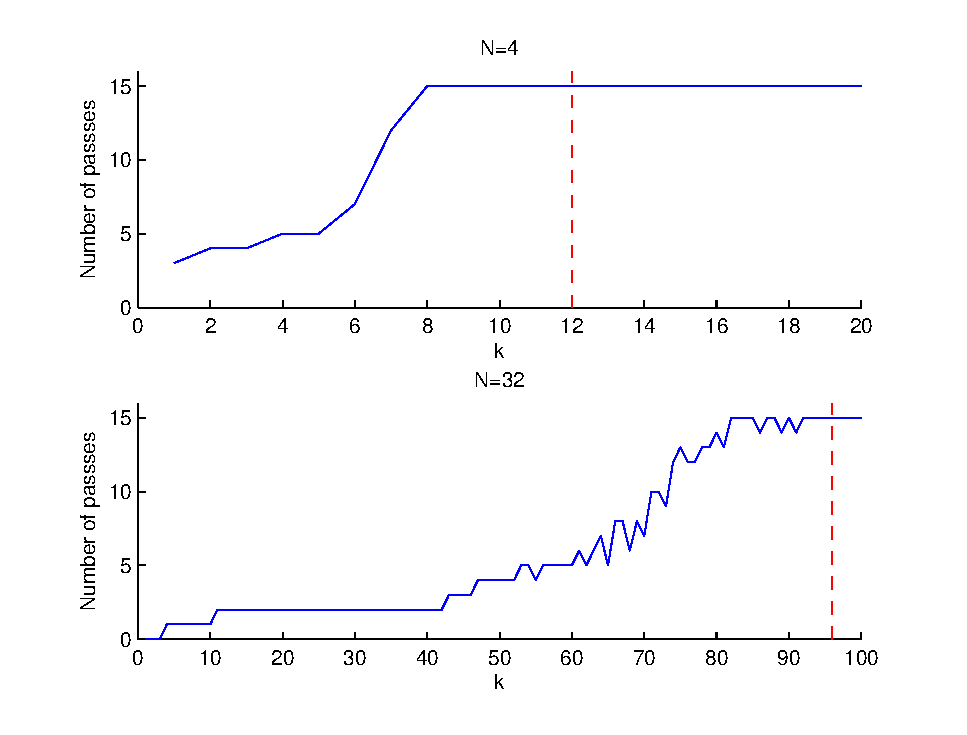
\includegraphics[scale=0.55]{images/correlation_c_sc.eps} 
\DeclareGraphicsExtensions.
\caption{Small Crush for CI(ISAAC,XORshift)}
\label{Small Crush for CI}
\end{figure}

\subsubsection{Correlation between TestU01 results and $\mathsf{N}$}

To compare the sequences generated with different parameters $\mathsf{N}$ in a more quantitative manner, we have set $k=3N+1$, and the same analysis for the four CI(X,Y) generators through TestU01 has been repeated. Let us recall that the TestU01 suite implements 518 tests and reports $p-$values, which must be within $[0.001,0.999]$ for a passing test.

\begin{figure*}
\centering
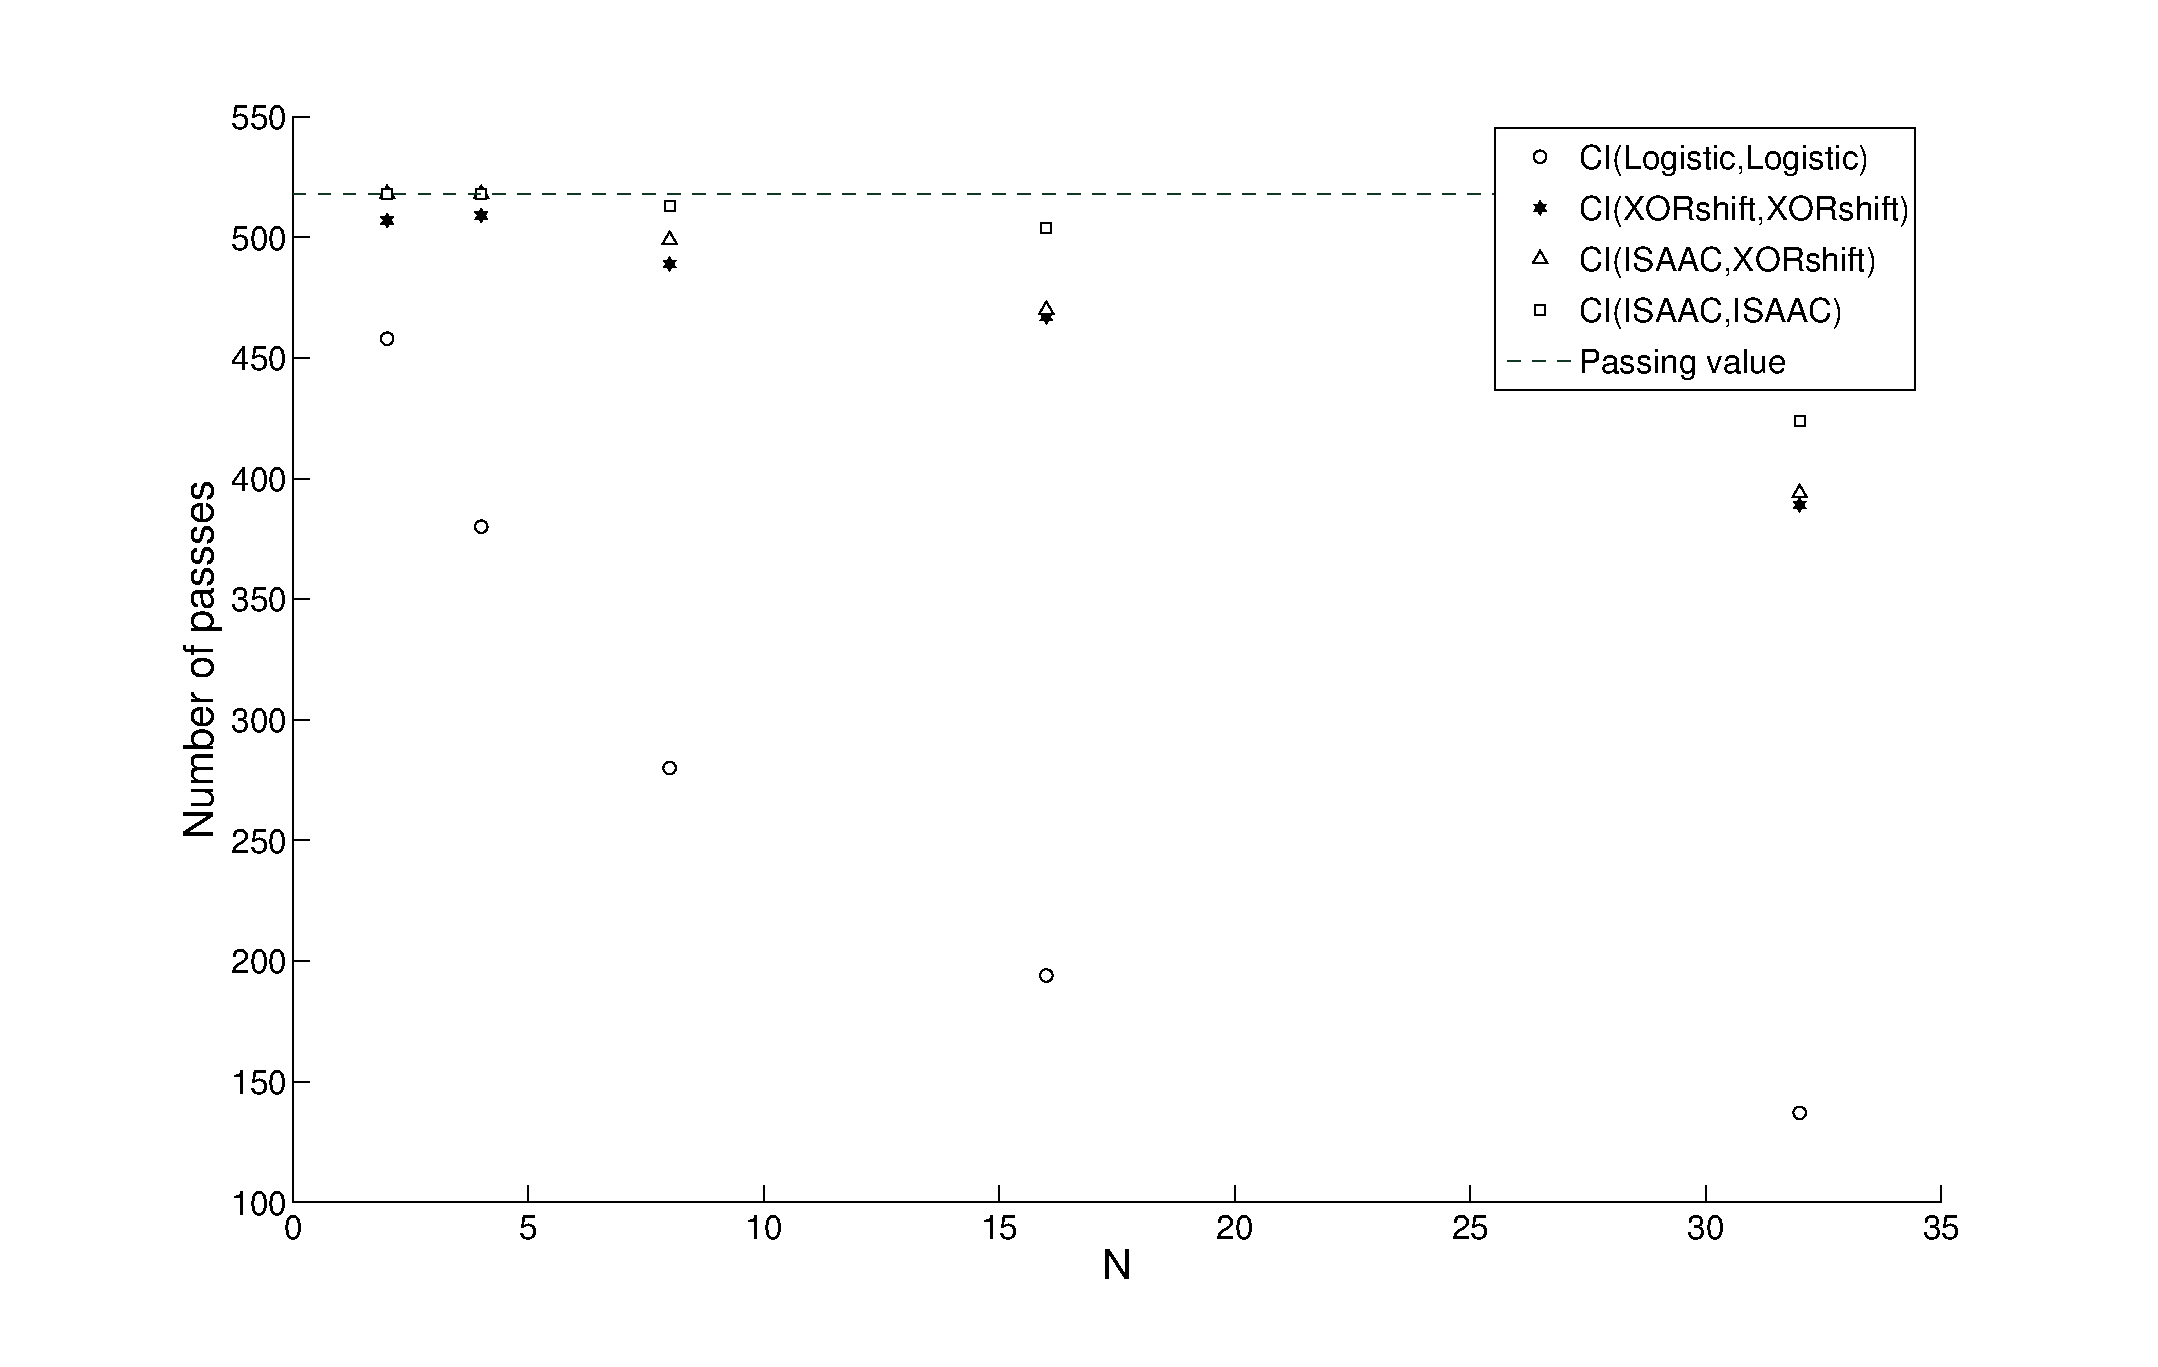
\includegraphics[scale=0.4]{images/N.eps} 
\DeclareGraphicsExtensions.
\caption{TestU01 results}
\label{TestU01 results}
\end{figure*}

Figure~\ref{TestU01 results} shows the number of passing sequences generated by the CI(X,Y) PRNGs proposed in this paper, with the same parameters and initial values. % (see the appendix for details).
It can be seen that $\mathsf{N}=4$ gives the best results.

For this reason, it is the default $\mathsf{N}=4$ with $k=12$ mode in following sections.
%As can be seen, the places where a sequence successfully passes most of the tests correspond nicely to the parameters for which $\mathsf{N}=4$.

\subsection{Results of NIST}

In our experiments, 100 sequences (s = 100) of 1,000,000 bits are generated and tested. If the value $\mathbb{P}_T$ of any test is smaller than 0.0001, the sequences are considered to not be good enough and the generator is unsuitable. Table~\ref{The passing for old CI} shows $\mathbb{P}_T$ of the sequences based on discrete chaotic iterations using different schemes. If there are at least two statistical values in a test, this test is marked with an asterisk and the average value is computed to characterize the statistical values. 


\begin{table}[!t]
\renewcommand{\arraystretch}{1.3}
\caption{NIST SP 800-22 test results ($\mathbb{P}_T$) for old CI algorithms ($\mathsf{N}=4$)}
\label{The passing for old CI}
\centering
  \begin{tabular}{lcccc}
    \toprule
\multirow{4}*{Test name} & \multicolumn{4}{c}{Old CI}\\
&Logistic& XORshift& ISAAC&ISAAC  \\ 
&+& +& + & + \\ 
&Logistic& XORshift& XORshift&ISAAC  \\ \cmidrule(r){2-5}
Frequency (Monobit) Test 			&0.85138	&0.59554	&0.40119		&0.33453 \\ 
Frequency Test within a Block  			&0.38382	&0.55442	&0.89776		&0.71974  \\ 
Runs Test 					&0.31908	&0.45593	&0.31908		&0.38382  \\ 
Longest Run of Ones in a Block Test 		&0.13728	&0.01671	&0.08558		&0.67868   \\
Binary Matrix Rank Test 			&0.69931	&0.61630	&0.47498		&0.79813  \\ 
Discrete Fourier Transform (Spectral) Test	&0.12962	&0.00019	&0.77918		&0.67868   \\ 
Non-overlapping Template Matching Test* 	&0.48473	&0.53225	&0.53568		&0.51258 \\ 
Overlapping Template Matching Test   		&0.47498	&0.33453	&0.36691		&0.07571  \\ 
Universal Statistical Test   			&0.09657	&0.03292	&0.26224		&0.85138   \\ 
Linear Complexity Test  			&0.41902	&0.40119	&0.61715		& 0.21330    \\ 
Serial Test* (m=10) 				&0.53427	&0.01339	&0.33453		&0.76102   \\ 
Approximate Entropy Test (m=10) 		&0.99146	&0.13728	&0.53414		&0.22482  \\ 
Cumulative Sums (Cusum) Test* 			&0.75530	&0.04646	&0.31915		& 0.47658\\ 
Random Excursions Test* 			&0.65406	&0.50362	&0.50804		&0.46305  \\ 
Random Excursions Variant Test* 		&0.55388	&0.34777	&0.48400		&0.54863    \\ \hline
Success 					&15/15		&15/15		&15/15		&15/15 \\ 
\bottomrule
  \end{tabular}
\end{table}


\subsection{Results of Diehard}
\label{Subsec:DieHARD}

Table~\ref{Results of DieHARD battery of tests for old CI algorithms} gives the results derived from applying the DieHARD battery of tests to the PRNGs considered in this work. 

\begin{tiny}
\begin{table}[!t]
\renewcommand{\arraystretch}{1.3}
\caption{Results of DieHARD battery of tests for old CI algorithms ($\mathsf{N}=4$)}
\label{Results of DieHARD battery of tests for old CI algorithms}
\centering
\begin{tabular}{llcccc} \toprule
\multirow{4}*{No.} &\multirow{4}*{Test name}& \multicolumn{4}{c}{Old CI}\\
&&Logistic& XORshift& ISAAC&ISAAC  \\ 
&&+& +& + & + \\ 
&&Logistic& XORshift& XORshift&ISAAC \\ \cmidrule(r){3-6}

1 & Overlapping Sum &Pass &Pass &Pass&Pass\\
2 & Runs Up 1 &Pass & Pass &Pass&Pass\\
&Runs Down 1 &Pass &Pass &Pass&Pass\\
&Runs Up 2 & Pass &Pass &Pass&Pass\\
&Runs Down 2 &Pass & Pass &Pass&Pass\\
3 & 3D Spheres &Pass &Pass &Pass&Pass\\
4 & Parking Lot &Pass &Pass &Pass&Pass\\
5 & Birthday Spacing &Pass &Pass &Pass&Pass\\
6 & Count the ones 1 &Pass &Pass &Pass&Pass\\
7 &Binary Rank $6 \times 8$ &Pass & Pass &Pass&Pass\\
8 &Binary Rank $31 \times 31$ &Pass &Pass &Pass&Pass\\
9 &Binary Rank $32 \times 32$ &Pass &Pass &Pass&Pass\\
10 &Count the ones 2 &Pass &Pass&Pass&Pass \\
11 &Bit Stream &Pass &Pass&Pass&Pass \\
12 &Craps Wins &Pass &Pass&Pass&Pass \\
&Throws &Pass &Pass &Pass&Pass\\
13 &Minimum Distance &Pass &Pass &Pass&Pass\\
14 &Overlapping Perm. &Pass &Pass &Pass&Pass\\
15 &Squeeze &Pass &Pass&Pass&Pass \\
16 &OPSO &Pass &Pass&Pass&Pass \\
17 &OQSO &Pass &Pass&Pass&Pass \\
18 &DNA &Pass &Pass&Pass &Pass\\
&Number of tests passed &18 &18 &18&18\\\bottomrule
\end{tabular}
\end{table}
\end{tiny}

\subsection{Results of comparative test parameters}

\begin{table}[!t]
\renewcommand{\arraystretch}{1.3}
\caption{Comparative test parameters for Old CI(X,Y) with a $10^7$ bits sequence ($\mathsf{N}=4$)}
\label{Comparison2 for old CI algorithms}
\centering
  \begin{tabular}{lccccc}
    \toprule
\multirow{4}*{Method} &\multirow{4}*{Threshold values} 	& \multicolumn{4}{c}{Old CI}\\
&&Logistic& XORshift& ISAAC&ISAAC  \\ 
&&+& +& + & + \\ 
&&Logistic& XORshift& XORshift&ISAAC \\ \cmidrule(r){3-6}
Monobit			&3.8415		&1.0368		&3.5689		&0.0569		&0.6641 \\ \hline
Serial  		&5.9915		&1.1758		&3.5765		&0.9828		&0.6506  \\ \hline
Poker  			&316.9194	&269.0607	&222.3683	&243.8415	&262.6440  \\ \hline
Runs 			&55.0027	&36.5479	&28.4237	&29.3195	&30.3116   \\ \hline
Autocorrelation		&1.6449		&0.4054		&0.3403		&0.6141		&0.9455  \\ \bottomrule
  \end{tabular}
\end{table}


We show in Table~\ref{Comparison2 for old CI algorithms} a comparison between old CI(Logistic, Logistic), old CI(XORshift, XORshift), old CI(ISAAC, XORshift), and old CI(ISAAC, ISAAC). %The comparative test is related to the duration needed by each algorithm to generate a $10^7$ bits long sequence. 


\subsection{Results of TestU01}
In a sound theoretical basis, a PRNG based on discrete chaotic iterations (CI) is a composite generator which combines the features of two PRNGs. The first generator constitutes the initial condition of the chaotic dynamical system. The second generator randomly chooses which outputs of the chaotic system must be returned. The intention of this combination is to cumulate the effects of chaotic and random behaviors, to improve the statistical and security properties relative to each generator taken alone.

This PRNG based on discrete chaotic iterations may utilize any reasonable RNG as inputs. For demonstration purposes, Logistic map, XORshift and ISAAC are adopted here. 

Table~\ref{TestU01 for old CI} gives the results derived from applying the TestU01 battery of tests to the PRNGs considered in this work.
\begin{table}[!t]
\renewcommand{\arraystretch}{1.3}
\caption{TestU01 Statistical Test for old CI algorithms ($\mathsf{N}=4$)}
\label{TestU01 for old CI}
\centering
  \begin{tabular}{lcccccc}
    \toprule
\multirow{4}*{Test name} &&& \multicolumn{4}{c}{Old CI}\\
&&&Logistic& XORshift& ISAAC&ISAAC  \\ 
&&&+& +& + & + \\ 
&&&Logistic& XORshift& XORshift&ISAAC  \\ \cmidrule(r){4-7}
Rabbit 				&$32\times10^9$ bits  	&38  	&7 	&2 	&0 	&0	 \\
Alphabit 			&$32\times10^9$ bits	&17 	& 3	&0 	&0 	&0	 \\
Pseudo DieHARD 			&Standard		&126 	&0 	&0 	&0 	&0	\\
FIPS\_140\_2 			&Standard		&16 	&0 	&0	&0 	&0	\\
Small Crush 			&Standard		&15 	&2 	&0	&0 	&0	 \\
Crush 				&Standard		&144 	&47 	&4 	&0 	&0	 \\
Big Crush 			&Standard		&160 	&79 	&3 	&0	&0	 \\ \hline
Number of failures 		& 			&518 	&138 	&9 	&0 	&0	 \\
\bottomrule
  \end{tabular}
\end{table}


\subsection{Conclusion}


Our old CI PRNG based on discrete chaotic iterations combines the features of two PRNGs, in order to improve their statistical properties. Logistic map, XORshift, and ISAAC are adopted here for demonstration purposes. 
The results of comparative test parameters confirm that the proposed CI PRNGs are all able to pass these tests.
Statistical results of comparative test parameters for both CI(XORshift, XORshift) and CI(ISAAC, XORshift) are better for most of the parameters, leading to the conclusion that these generators are more secure than the others. 
This improvement clearly appears in the TestU01 results: i.e. XORshift alone fails 142 of these tests, whereas  CI(XORshift, XORshift) only fails 9 out of 518.
In other words, in addition of having chaotic properties, our PRNG based on discrete chaotic iterations can pass more performed tests than its individual components taken alone. 


\section{Test results and comparative analysis for new CI}

\subsection{Results of NIST}
\label{Results of NISTfor new CI}
In our experiments, 100 sequences (s = 100) of 1,000,000 bits are generated and tested. If the value $\mathbb{P}_T$ of any test is smaller than 0.0001, the sequences are considered to not be good enough and the generator is unsuitable. Table~\ref{The passing rate1} and Table~\ref{The passing for new CI} show $\mathbb{P}_T$ of the sequences based on discrete chaotic iterations using different schemes. If there are at least two statistical values in a test, this test is marked with an asterisk and the average value is computed to characterize the statistical values. 

\begin{table}[!t]
\renewcommand{\arraystretch}{1.3}
\caption{SP 800-22 test results ($\mathbb{P}_T$) for new CI(XORshift, XORshift)  $\mathsf{N}=32$}
\label{The passing rate1}
\centering
\begin{tabular}{lcccc}
    \toprule
\multirow{2}*{Method} & \multicolumn{3}{c}{New CI}\\
 & $m^n=y^n~mod~N$&no mark&$g_2()$\\ \cmidrule(r){2-4}
%$w^{j}$ & $\{1,..,8\}$ & $\{1,..,8\}$ & $\{1,..,8\}$ & $\{1,..,5\}$ & $\{1,..,5\}$ &$\{1,..,5\}$ \\ \hline \hline
Frequency (Monobit) Test 			&0.00040	&0.08556		&0.41943\\ 
Frequency Test within a Block  			&0		&0			&0.67862\\ 
Runs Test  					&0.28966	&0.55448		&0.33452\\ 
Longest Run of Ones in a Block Test 		&0.01096	&0.43723		&0.88313 \\ 
Binary Matrix Rank Test  			&0		&0.65794		&0.75972\\ 
Discrete Fourier Transform (Spectral) Test 	&0		&0			&0.00085 \\ 
Non-overlapping Template Matching Test* 	&0.02007	&0.37333		&0.51879\\ 
Overlapping Template Matching Test		&0		&0	 	 	&0.24924\\ 
Maurer's ``Universal Statistical'' Test  	&0.69936	&0.96424		&0.12963\\ 
Linear Complexity Test 				&0.36699	&0.92423	 	&0.35045\\ 
Serial Test* (m=10) 				&0		&0.28185	 	&0.25496\\ 
Approximate Entropy Test (m=10) 		&0		&0.38381	 	&0.75971\\ 
Cumulative Sums (Cusum) Test* 			&0		&0			&0.34245\\ 
Random Excursions Test* 			&0.46769	&0.34788	 	&0.18977\\ 
Random Excursions Variant Test* 		&0.28779	&0.46505		&0.26563\\ \hline
Success 					&8/15		&11/15		  	&15/15\\ 
\bottomrule
\end{tabular}
\end{table}

We can conclude from Table \ref{The passing rate1} that the worst situations are obtained with the New CI ($m^n=y^n~mod~N$) and New CI (no mark) generators. %: they just can be observed that 8 and 11 out of 15 of the tests are failed. However,
New CI ($m^n=g_2(y^n)$) as New CI ($m^n=g_1(y^n)$) in Table~\ref{The passing for new CI} has successfully passed the NIST statistical test suite.

\begin{table}[!t]
\renewcommand{\arraystretch}{1.3}
\caption{NIST SP 800-22 test results ($\mathbb{P}_T$) for new CI algorithms}
\label{The passing for new CI}
\centering
  \begin{tabular}{lccc}
    \toprule
\multirow{4}*{Test name} & \multicolumn{3}{c}{New CI}\\
& XORshift& ISAAC&ISAAC  \\ 
& +& + & + \\ 
& XORshift& XORshift&ISAAC  \\  \cmidrule(r){2-4}
Frequency (Monobit) Test 			&0.47498 		&0.88317		&0.83430 \\ 
Frequency Test within a Block  			&0.89776		&0.40119		&0.33453  \\ 
Runs Test 					&0.81653		&0.31908		&0.00576  \\ 
Longest Run of Ones in a Block Test 		&0.79813		&0.06688		&0.47498   \\
Binary Matrix Rank Test 			&0.26224		&0.88317		&0.69931  \\ 
Discrete Fourier Transform (Spectral) Test	&0.00716		&0.33453		&0.59559   \\ 
Non-overlapping Template Matching Test* 	&0.44991		&0.46467		&0.51446 \\ 
Overlapping Template Matching Test   		&0.51412		&0.69931		&0.88317  \\ 
Universal Statistical Test   			&0.67868		&0.24928		&0.06282   \\ 
Linear Complexity Test  			&0.65793		&0.65793		&0.94630     \\ 
Serial Test* (m=10) 				&0.42534		&0.90619		&0.44137   \\ 
Approximate Entropy Test (m=10) 		&0.63719		&0.22482		&0.13728  \\ 
Cumulative Sums (Cusum) Test* 			&0.27968		&0.84065		&0.14139 \\ 
Random Excursions Test* 			&0.28740		&0.30075		&0.34625   \\ 
Random Excursions Variant Test* 		&0.48668		&0.34294		&0.55048    \\ \hline
Success 					& 15/15			&15/15		&15/15	 \\ 
\bottomrule
  \end{tabular}
\end{table}

\subsection{Results of Diehard}
\label{Subsec:DieHARD}

Table~\ref{Results of DieHARD battery of tests for new CI algorithms} gives the results derived from applying the DieHARD battery of tests to the PRNGs considered in this work. 

\begin{tiny}
\begin{table}[!t]
\renewcommand{\arraystretch}{1.3}
\caption{Results of DieHARD battery of tests for new CI algorithms ($\mathsf{N}=32$)}
\label{Results of DieHARD battery of tests for new CI algorithms}
\centering
\begin{tabular}{llcccc} \toprule
\multirow{3}*{No.} &\multirow{3}*{Test name} & \multicolumn{4}{c}{New CI}\\
&&Logistic& XORshift& ISAAC&ISAAC  \\ 
&&+& +& + & + \\ 
&&Logistic& XORshift& XORshift&ISAAC \\ \cmidrule(r){3-6}
1 & Overlapping Sum &Pass &Pass &Pass&Pass\\
2 & Runs Up 1 &Pass & Pass &Pass&Pass\\
&Runs Down 1 &Pass &Pass &Pass&Pass\\
&Runs Up 2 & Pass &Pass &Pass&Pass\\
&Runs Down 2 &Pass & Pass &Pass&Pass\\
3 & 3D Spheres &Pass &Pass &Pass&Pass\\
4 & Parking Lot &Pass &Pass &Pass&Pass\\
5 & Birthday Spacing &Pass &Pass &Pass&Pass\\
6 & Count the ones 1 &Pass &Pass &Pass&Pass\\
7 &Binary Rank $6 \times 8$ &Pass & Pass &Pass&Pass\\
8 &Binary Rank $31 \times 31$ &Pass &Pass &Pass&Pass\\
9 &Binary Rank $32 \times 32$ &Pass &Pass &Pass&Pass\\
10 &Count the ones 2 &Pass &Pass&Pass&Pass \\
11 &Bit Stream &Pass &Pass&Pass&Pass \\
12 &Craps Wins &Pass &Pass&Pass&Pass \\
&Throws &Pass &Pass &Pass&Pass\\
13 &Minimum Distance &Pass &Pass &Pass&Pass\\
14 &Overlapping Perm. &Pass &Pass &Pass&Pass\\
15 &Squeeze &Pass &Pass&Pass&Pass \\
16 &OPSO &Pass &Pass&Pass&Pass \\
17 &OQSO &Pass &Pass&Pass&Pass \\
18 &DNA &Pass &Pass&Pass &Pass\\
&Number of tests passed &18 &18 &18&18\\\bottomrule
\end{tabular}
\end{table}
\end{tiny}

\subsection{Results of comparative test parameters}



\begin{table}[!t]
\renewcommand{\arraystretch}{1.3}
\caption{Comparative test parameters for new CI(X,Y) with a $10^7$ bits sequence ($\mathsf{N}=32$)}
\label{Comparison2 for new CI algorithms}
\centering
  \begin{tabular}{lcccc}
    \toprule
\multirow{4}*{Method} &\multirow{4}*{Threshold values} 	& \multicolumn{3}{c}{New CI}\\
&& XORshift& ISAAC&ISAAC  \\ 
&& +& + & + \\ 
&& XORshift& XORshift&ISAAC \\ \cmidrule(r){2-5}
Monobit			&3.8415				&3.5689		&0.9036		&0.5788 \\ \hline
Serial  		&5.9915				&3.5765		&1.1229		&0.7378  \\ \hline
Poker  			&316.9194			&123.6831	&173.8604		&179.8609  \\ \hline
Runs 			&55.0027			&28.4237	&40.4606	&29.4057   \\ \hline
Autocorrelation		&1.6449				&0.3403		&0.1245		&-2.0276 \\ \bottomrule
  \end{tabular}
\end{table}

We show in Table~\ref{Comparison2 for new CI algorithms} a comparison between New CI(XORshift, XORshift), New CI(ISAAC, XORshift), and New CI(ISAAC, ISAAC). %The comparative test is related to the duration needed by each algorithm to generate a $10^7$ bits long sequence. 

\subsection{Results of TestU01}


Table~\ref{TestU01 for new CI} gives the results derived from applying the TestU01 battery of tests to the PRNGs considered in this work.
\begin{table}[!t]
\renewcommand{\arraystretch}{1.3}
\caption{TestU01 Statistical Test for new CI algorithms ($\mathsf{N}=32$)}
\label{TestU01 for new CI}
\centering
  \begin{tabular}{lccccc}
    \toprule
\multirow{4}*{Test name} &&& \multicolumn{3}{c}{New CI}\\
&&&Logistic& ISAAC&ISAAC  \\ 
&&&+& +& + \\ 
&&&Logistic& XORshift&ISAAC  \\ \cmidrule(r){4-6}
Rabbit 				&$32\times10^9$ bits  	&38  	&0 	&0 	&0 		 \\
Alphabit 			&$32\times10^9$ bits	&17 	&0 	&0 	&0 		 \\
Pseudo DieHARD 			&Standard		&126 	&0 	&0 	&0 		\\
FIPS\_140\_2 			&Standard		&16 	&0 	&0 	&0 		\\
Small Crush 			&Standard		&15 	&0	&0	&0 		 \\
Crush 				&Standard		&144 	&0 	&0 	&0 		 \\
Big Crush 			&Standard		&160 	&0 	&0 	&0		 \\ \hline
Number of failures 		& 			& 	&0 	&0	&0 		 \\
\bottomrule
  \end{tabular}
\end{table}


\subsection{Conclusion}
In a sound theoretical basis, a New PRNG based on discrete chaotic iterations (CI) is a composite generator which combines the features of two PRNGs. The first generator constitutes the initial condition of the chaotic dynamical system. The second generator randomly chooses which outputs of the chaotic system must be returned. The intention of this combination is to cumulate the effects of chaotic and random behaviors, to improve the statistical and security properties relative to each generator taken alone.

This New CI PRNG based on discrete chaotic iterations may utilize any reasonable RNG as inputs. For demonstration purposes, XORshift and ISAAC are adopted here. 

The results of the TestU01, NIST, Comparative test parameters and DieHARD batteries of tests confirm that the proposed New CI PRNGs are all able to pass these tests. And it is better than Old CI algorithms

The improvement clearly appears in the TestU01 results: i.e. XORshift alone fails 142 of these tests, whereas  Old CI(XORshift, XORshift) fails 9 out of 518, New CI(XORshift, XORshift) can pass all the tests. 

Detail comparative analysis will be presented in the next section.


\section{Assessment of two chaotic iterations schemes based on XORshift Generator}

\subsection{NIST}

In our experiments, 100 sequences (s = 100) of 1,000,000 bits are generated and tested. If the value $\mathbb{P}_T$ of any test is smaller than 0.0001, the sequences are considered to not be good enough and the generator is unsuitable. Table~\ref{The passing} shows $\mathbb{P}_T$ of the sequences based on discrete chaotic iterations using different schemes. If there are at least two statistical values in a test, this test is marked with an asterisk and the average value is computed to characterize the statistical values. 
We can conclude from Table \ref{The passing} that XORshift has failed 1 test, whereas both the old generator and CI(XORshift, XORshift) have successfully passed the NIST statistical test suite. This result shows the good behavior of both PRNGs in the aforementioned basic tests that evaluate the independence of real numbers.

\begin{table}[!t]
\renewcommand{\arraystretch}{1.3}
\caption{NIST SP 800-22 test results ($\mathsf{N}=32$)}
\label{The passing}
\centering
  \begin{tabular}{|l||c|c|c|}
    \hline
Method &XORshift& Old CI & New CI  \\ \hline\hline

Frequency (Monobit) Test 			&0.145326&0.595549&0.474986 \\ \hline
Frequency Test within a Block  			&0.455937&0.554420&0.897763  \\ \hline
Runs Test 					&0.213309&0.455937&0.816537 \\ \hline
Longest Run of Ones in a Block Test 		&0.289667&0.016717&0.798139   \\ \hline
Binary Matrix Rank Test 			&0.000000&0.616305&0.262249  \\ \hline
Discrete Fourier Transform (Spectral) Test	&0.005358&0.000190&0.007160   \\ \hline
Non-overlapping Template Matching Test* 	&0.503652&0.532252&0.449916 \\ \hline
Overlapping Template Matching Test   		&0.867692&0.334538&0.514124  \\ \hline
Universal Statistical Test   			&0.275709&0.032923&0.678686  \\ \hline
Linear Complexity Test  			&0.924076&0.401199&0.657933    \\ \hline
Serial Test* (m=10) 				&0.757925&0.013396&0.425346  \\ \hline
Approximate Entropy Test (m=10) 		&0.419021&0.137282&0.637119  \\ \hline
Cumulative Sums (Cusum) Test* 			&0.8115445&0.046464&0.279680\\ \hline
Random Excursions Test* 			&0.4192395&0.503622&0.287409   \\ \hline
Random Excursions Variant Test* 		&0.5283333&0.347772&0.486686    \\ \hline
Success 					& 14/15	  & 15/15  & 15/15 \\ \hline

  \end{tabular}
\end{table}

\subsection{Diehard}
\label{Subsec:DieHARD}

Table~\ref{Results of DieHARD battery of tests} gives the results derived from applying the DieHARD battery of tests to the PRNGs considered in this work. As it can be observed, the results of the individual tests Count the ones 1, Binary Rank $31 \times 31$ and Binary Rank $32 \times 32$ show that in the random numbers obtained with the XORshift generator only the least significant bits seem to be independent. This explains the poor behavior of this PRNG in the aforementioned basic tests that evaluate the independence of real numbers. But the generator based on discrete chaotic iterations (New CI and Old CI PRNG) can pass all the DieHARD battery of tests. 
This proves that the
security of the given generator has been improved by chaotic iterations.

\begin{tiny}
\begin{table}[!t]
\renewcommand{\arraystretch}{1.3}
\caption{Results of DieHARD battery of tests ($\mathsf{N}=32$)}
\label{Results of DieHARD battery of tests}
\centering
\begin{tabular}{llccc} \toprule
\textbf{No.} &\textbf{Test name} &\multicolumn{3}{c}{\textbf{Generators}} \\ \cmidrule(r){3-5}
& & XORshift &  Old CI & New CI\\ \midrule
1 & Overlapping Sum &Pass &Pass &Pass\\
2 & Runs Up 1 &Pass & Pass &Pass\\
&Runs Down 1 &Pass &Pass &Pass\\
&Runs Up 2 & Pass &Pass &Pass\\
&Runs Down 2 &Pass & Pass &Pass\\
3 & 3D Spheres &Pass &Pass &Pass\\
4 & Parking Lot &Pass &Pass &Pass\\
5 & Birthday Spacing &Pass &Pass &Pass\\
6 & Count the ones 1 &Fail &Pass &Pass\\
7 &Binary Rank $6 \times 8$ &Pass & Pass &Pass\\
8 &Binary Rank $31 \times 31$ &Fail &Pass &Pass\\
9 &Binary Rank $32 \times 32$ &Fail &Pass &Pass\\
10 &Count the ones 2 &Pass &Pass&Pass \\
11 &Bit Stream &Pass &Pass&Pass \\
12 &Craps Wins &Pass &Pass&Pass \\
&Throws &Pass &Pass &Pass\\
13 &Minimum Distance &Pass &Pass &Pass\\
14 &Overlapping Perm. &Pass &Pass &Pass\\
15 &Squeeze &Pass &Pass&Pass \\
16 &OPSO &Pass &Pass&Pass \\
17 &OQSO &Pass &Pass&Pass \\
18 &DNA &Pass &Pass&Pass \\
&Number of tests passed &15 &18 &18\\\bottomrule
\end{tabular}
\end{table}
\end{tiny}

\subsection{Comparative test parameters}

\begin{table}
\renewcommand{\arraystretch}{1.3}
\caption{Comparison with Old CI(XORshift,XORshift) for a $2 \times 10^5$ bits sequence  ($\mathsf{N}=32$)}
\label{Comparison22}
\centering
  \begin{tabular}{lcccc}
    \toprule
Method &The threshold values&XORshift& Old CI& New CI \\ \hline
   
Monobit			&3.8415		&1.7053		&2.7689		&0.3328	 \\ \hline
Serial  		&5.9915		&2.1466		&2.8765		&0.7441		  \\ \hline
Poker  			&316.9194	&248.9318	&222.3683	&262.8173		 \\ \hline
Runs 			&55.0027	&18.0087	&21.9272	&16.7877	   \\ \hline
Autocorrelation		&1.6449		&0.5009		&0.0173		&0.0805		  \\ \hline
Time			&Second		&0.096s		&0.3625s	&0.197s		  \\ 
    \bottomrule
  \end{tabular}
\end{table}



We show in Table~\ref{Comparison22} a comparison between our new generator New CI(XORshift, XORshift), its old version denoted Old CI(XORshift, XORshift), and a PRNG based on a simple XORshift. Time (in seconds) is related to the duration needed by each algorithm to generate a $2 \times 10^5$ bits long sequence. The test has been conducted using the same computer and compiler with the same optimization settings for both algorithms, in order to make it as fair as possible. 
The results confirm that the proposed generator is a lot faster than the old one, while the statistical results are better for most of the parameters, leading to the conclusion that the new PRNG is more secure than the old one. % The main advantage of our new method lies in its flexibility, therefore optimizing for higher speeds, better security or low memory requirements.


\begin{figure}
\centering
% \psfig{figure=2.eps,height=5in,width=3.5in}
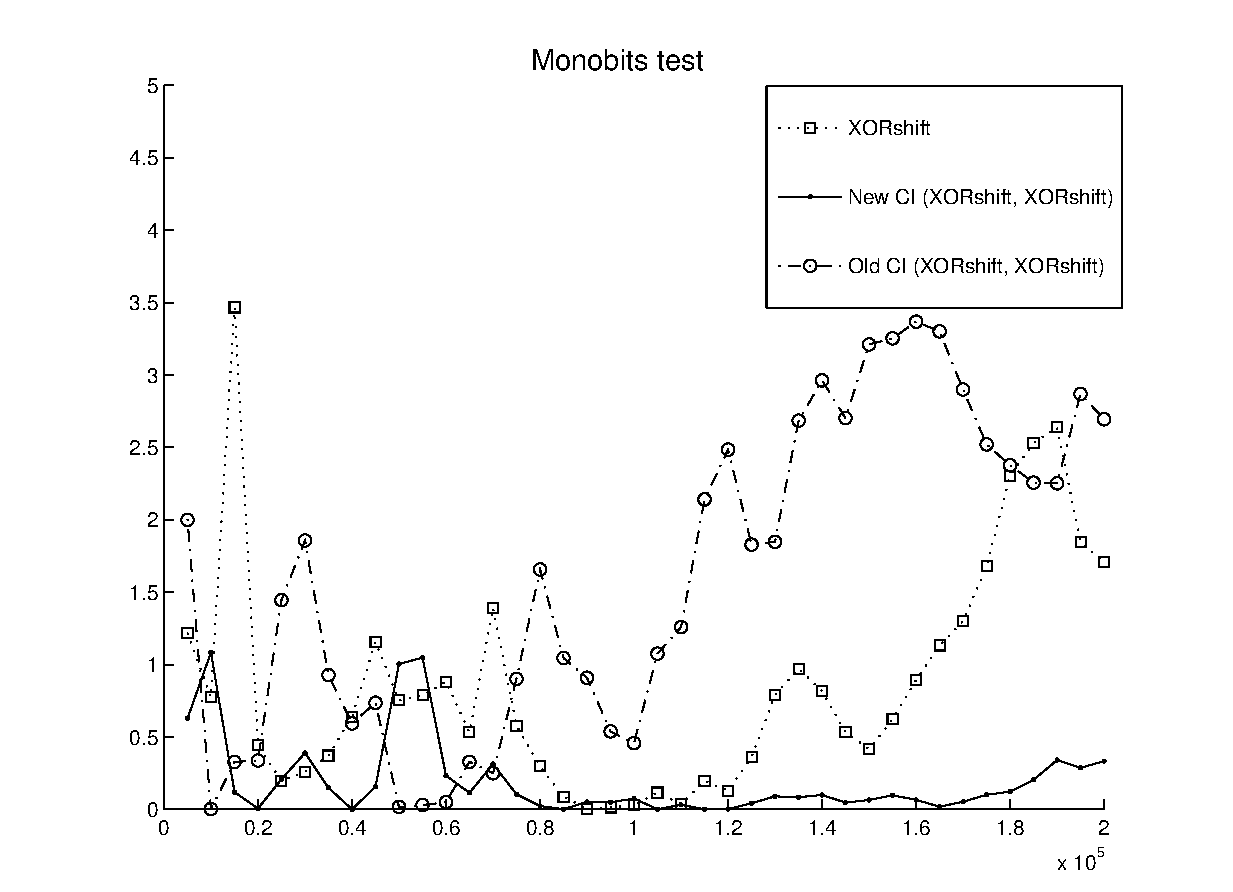
\includegraphics[scale=0.4]{monobits.eps}
% \includegraphics[width=3.7in]{4tests.eps}
\caption{Comparison of monobits tests}
\label{monobits}
\end{figure}

As a comparison of the overall stability of these PRNGs, similar tests have been computed for different sequence lengths (see Figures \ref{monobits} - \ref{autocorrelation}).
For the monobit test comparison (Figure \ref{monobits}), XORshift and New CI(XORshift, XORshift) PRNGs present the same issue: the beginning values are a little high. However, for our new generator, the values are stable in a low level which never exceeds 1.2. Indeed, the new generator distributes very randomly the zeros and ones, whatever the length of the desired sequence. 
It can also be remarked that the old generator presents the worst performance, but the values are  still within the standard boundary.
% The main advantage of our new method lies in its flexibility, therefore optimizing for higher speeds, better security or low memory requirements.

\begin{figure}
\centering
% \psfig{figure=2.eps,height=5in,width=3.5in}
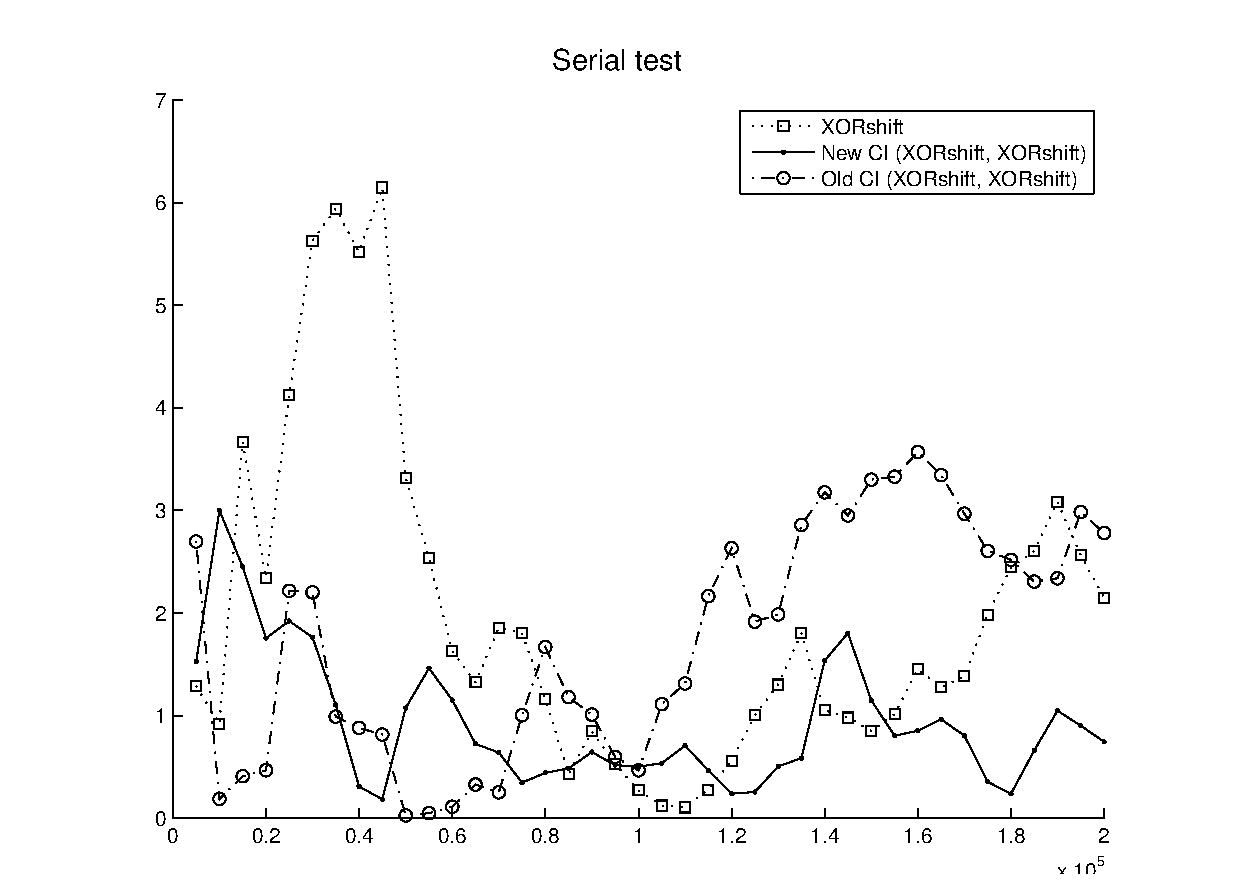
\includegraphics[scale=0.4]{serial.eps}
% \includegraphics[width=3.7in]{4tests.eps}
\caption{Comparison of serial tests}
\label{serial}
\end{figure}

Figure \ref{serial} shows the serial test comparison. The new generator outperforms this test, but the score of the old generator is not bad either: their occurrences of 00, 01, 10, and 11 are very close to each other.% As the same with monobit test, this phenomenon is attributed to the effect of iteration computation.

\begin{figure}
\centering
% \psfig{figure=2.eps,height=5in,width=3.5in}
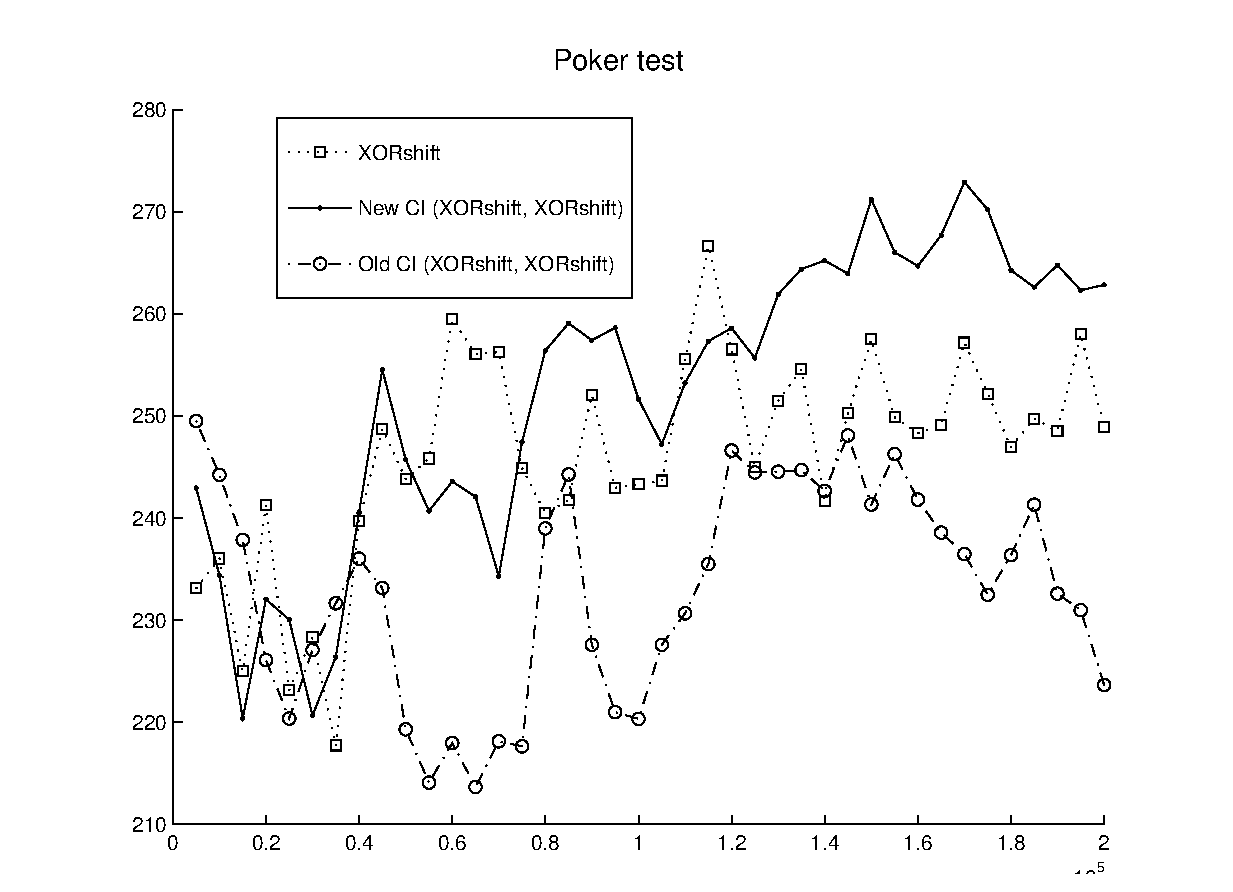
\includegraphics[scale=0.4]{poker.eps}
% \includegraphics[width=3.7in]{4tests.eps}
\caption{Comparison of poker tests}
\label{poker}
\end{figure}

The poker test comparison with $m=8$ is shown in Figure \ref{poker}. XORshift is the most stable generator in all of these tests, but not better than Old CI(XORshift, XORshift) PRNG. 
Our new generator presents a trend, with a maximum in the neighborhood of $1.7 \times 10^5$. These scores are not so good, even though the new generator has a better behavior than the old one and XORshift. 
%The reasons explaining this bad result can be, among other:
Indeed, the value of $m$ and the length of the sequences should be enlarged to be certain that the chaotic iterations express totally their complex behavior. In that situation, the performances of our generators in the poker test can be improved.
%but here we only achieve $2 \times 10^5$ sequence length, then m must be smaller than 13 to comply with the rule, if the sequence length is more, the performance of CI might be better.

\begin{figure}
\centering
% \psfig{figure=2.eps,height=5in,width=3.5in}
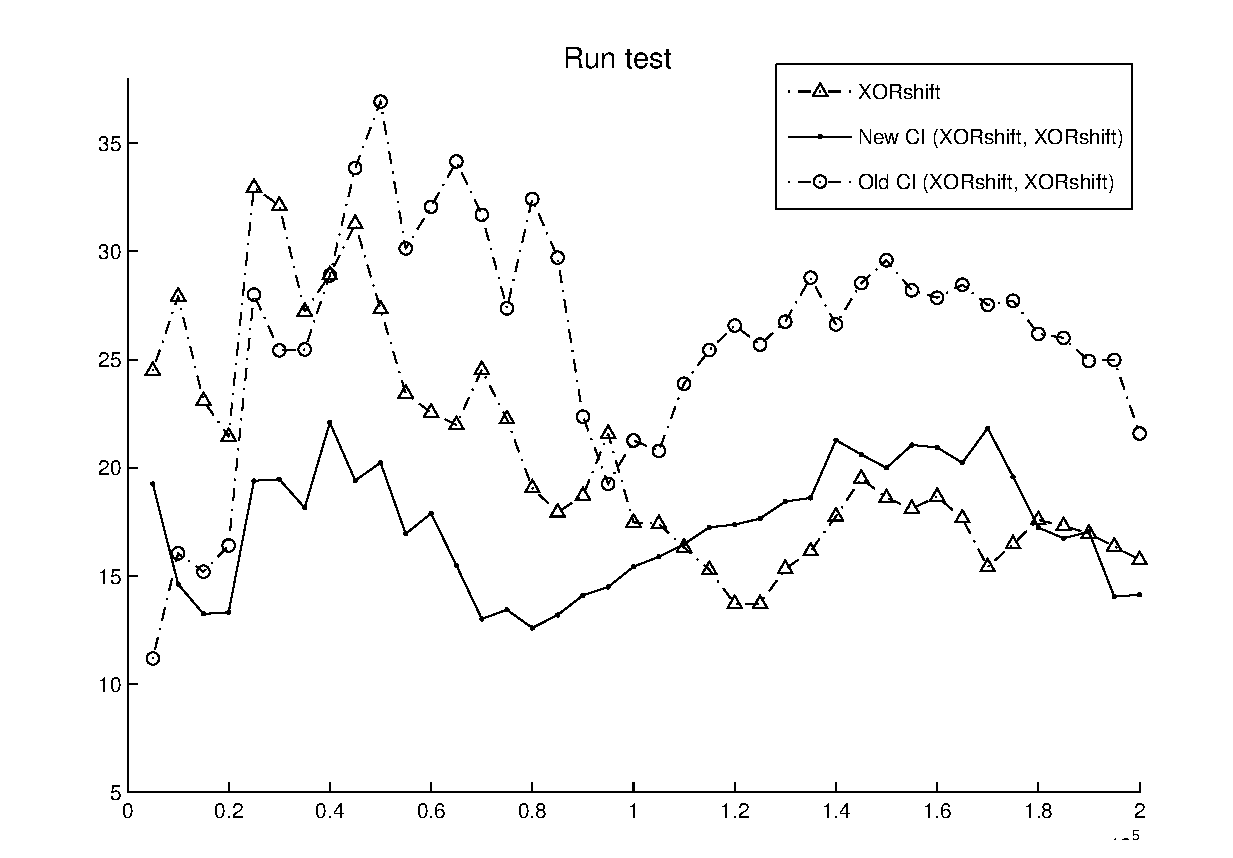
\includegraphics[scale=0.4]{runs.eps}
% \includegraphics[width=3.7in]{4tests.eps}
\caption{Comparison of runs tests}
\label{runs}
\end{figure}

The graph of the new generator is the most stable one during the runs test comparison (Figure \ref{runs}). Moreover, this trend is reinforced when the lengths of the tested sequences are increased.


\begin{figure}
\centering
% \psfig{figure=2.eps,height=5in,width=3.5in}
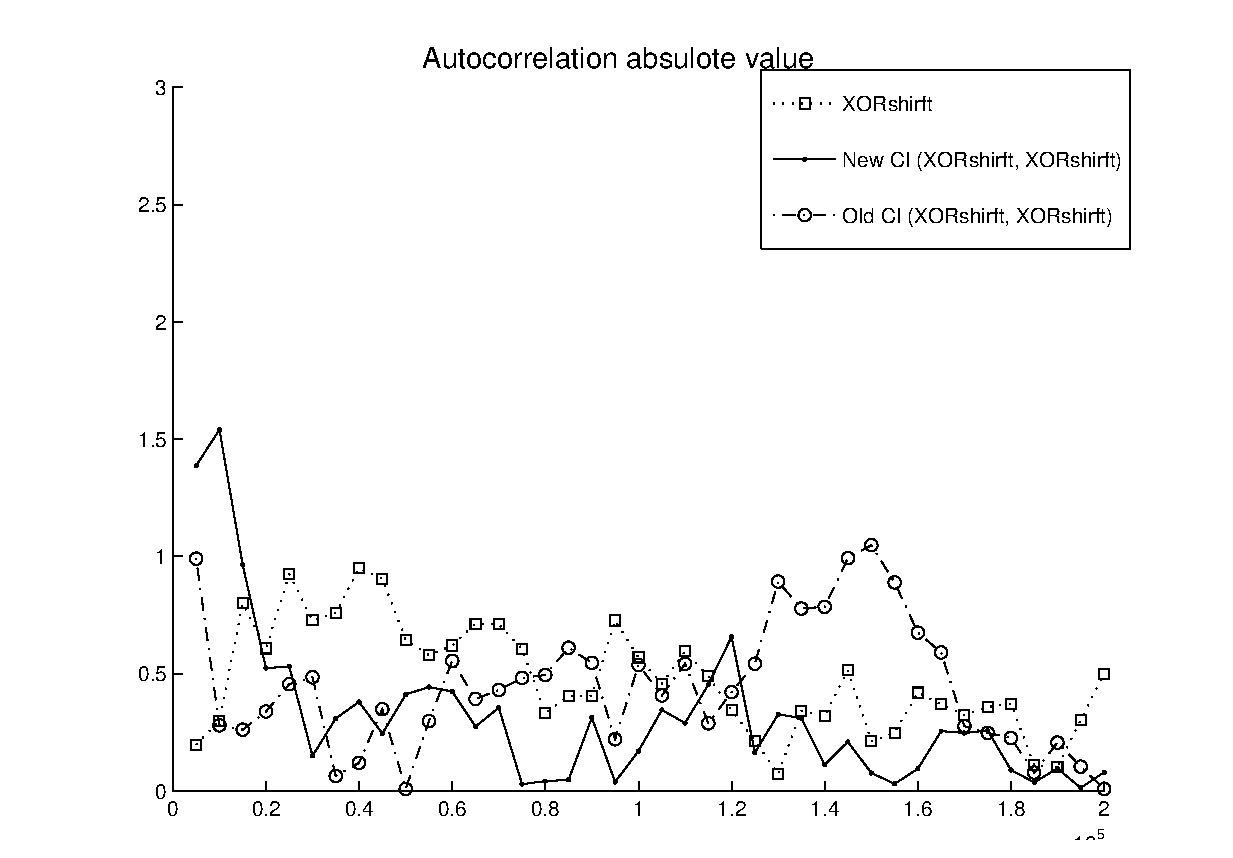
\includegraphics[scale=0.4]{autocorrelation1.eps}
% \includegraphics[width=3.7in]{4tests.eps}
\caption{Comparison of autocorrelation tests}
\label{autocorrelation}
\end{figure}


The comparison of autocorrelation tests is presented in Figure \ref{autocorrelation}. The new generator clearly dominates these tests, whereas the score of the old generator is also not bad. This difference between two generators based on chaotic iterations can be explained by the fact that the improvements realized to define the new generator lead to a more randomly output.

To sum up we can claim that the new generator, which is faster than its former version, outperforms all of the other generators in these statistical tests, especially when producing long output sequences.




\subsection{A flexible output}

We assume that the initial state $X$ is given as arrays of N-bit integers. Thus, the output size can be flexibly chosen  as well as $N$. Our PRNGs can generate discrete numbers
where the number of states could not match to a power of 2, which is suitable for stochastic differential equations as an example.(An attractive property of discrete random numbers is that they
require a small number of random bits--3 bits)~\cite{Ladd20092140}.
Moreover, due to the fact that CI process is a simple bitwise change, the speed of output integers and binary numbers is almost the same. 

In the following section, we will discuss the security level for various $N$ by Statistical test.
For both CI generator, various $N$ can pass all the NIST and DIEHARD test. Table~\ref{TestU01 Statistical Test} gives the results derived from applying the TestU01 battery of tests to the PRNGs considered in this work. As observed,  we can conclude that the effective range of $N$ for new CI is bigger than for old CI by TestU01. And also, this new scheme for obtaining a PRNG by combining two XORshift generators in CI give better properties than the old one (and the individual XORshift alone). It can be observed that the XORshift generator fails 146 tests.

\begin{table}[!t]
\begin{small}
\centering
\renewcommand{\arraystretch}{1.3}
\caption{TestU01 Statistical Test}
\label{TestU01 Statistical Test}
\centering
\begin{tabular}{cccccccccc}\toprule
\textbf{CI PRNG}&\textbf{Battery}&\textbf{N=2}&\textbf{N=4}&\textbf{N=8}&\textbf{N=16}&\textbf{N=32} \\\midrule

\multirow{7}*{\textbf{Old CI}}&Rabbit  					 	&2	&2	&2	&2	&3 \\
\multirow{7}*{\textbf{(XORshift,XORshift)}}&Alphabit 				&0	&0	&0	&2	&2 \\
&Pseudo DieHARD 								&0	&0	&0	&0	&0 \\
&FIPS\_140\_2 		 							&0	&0	&0	&0	&0 \\
&Small Crush 		 							&0	&0	&0	&1	&0 \\
&Crush 		 								&4	&4	&9	&16	&46 \\
&Big Crush 									&5	&3	&18	&30	&78 \\ 
\\
&Number of failures 	 							&11	&9	&29	&51	&129 \\
\bottomrule

\multirow{7}*{\textbf{New CI}}&Rabbit 					  	&0	&0	&0	&0	&0 \\
\multirow{7}*{\textbf{(XORshift,XORshift)}}&Alphabit 				&4	&0	&0	&0	&0 \\
&Pseudo DieHARD 	 							&8	&2	&0	&0	&0 \\
&FIPS\_140\_2		 							&2	&0	&0	&0	&0 \\
&Small Crush 		 							&0	&0	&0	&0	&0 \\
&Crush 										&0	&0	&0	&0	&0 \\
&Big Crush 		 							&0	&0	&0	&0	&0 \\ 
\\
&Number of failures 	 							&14	&2	&0	&0	&0 \\
\bottomrule
\end{tabular}
\end{small}
\end{table}




\chapter{Performance Evaluation}
\label{Performance Evaluation}
\minitoc

Although non-uniform distributed random numbers may be needed in some applications,
for example the user request generator with non-uniform distributed arrival rate in a queuing
system, it is still a majority to have a random sequence with uniform distribution over certain
domain S (this kind of random number generator is called uniform random number generator). 
In order to test the uniformity of a sequence, several methods can be applied.

\section{Balance of Probability}


If a bit sequence is concerned, the uniformity can be justified by comparing the
number of 0's and 1's appeared. That can be accounted with the balance of probability [19],
which defined as$\frac{p-q}{n}$, where $p$ and $q$ are the occurrence frequencies of ``1`` and ``0``,
respectively and $n$ is the number of bits. Figure~\ref{Balance of Probability for old CI} and Figure~\ref{Balance of Probability for new CI} show the balance of probability for a bit
sequence generated by chaotic iterations, showing that the chances to have ``0`` and ``1`` are more or less
the same.
\begin{figure}
\centering
\subfigure[Old CI(Logistic, Logistic)]{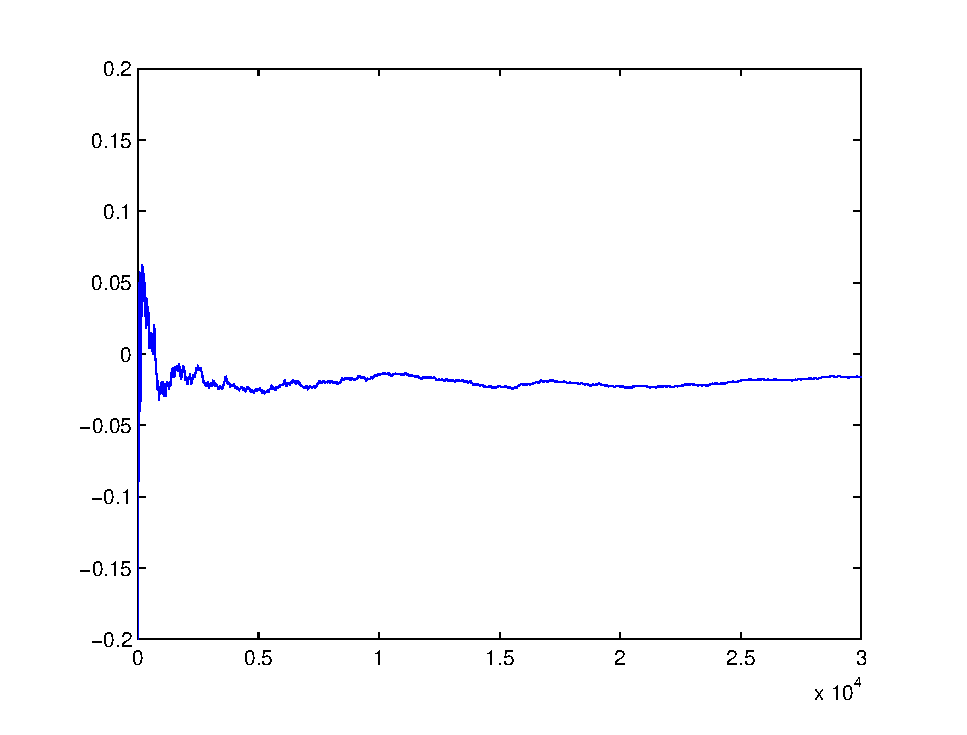
\includegraphics[scale=0.34]{images/balance_oldci_ll.eps}
} \hspace{0.5cm}
\subfigure[Old CI(XORshift, XORshift)]{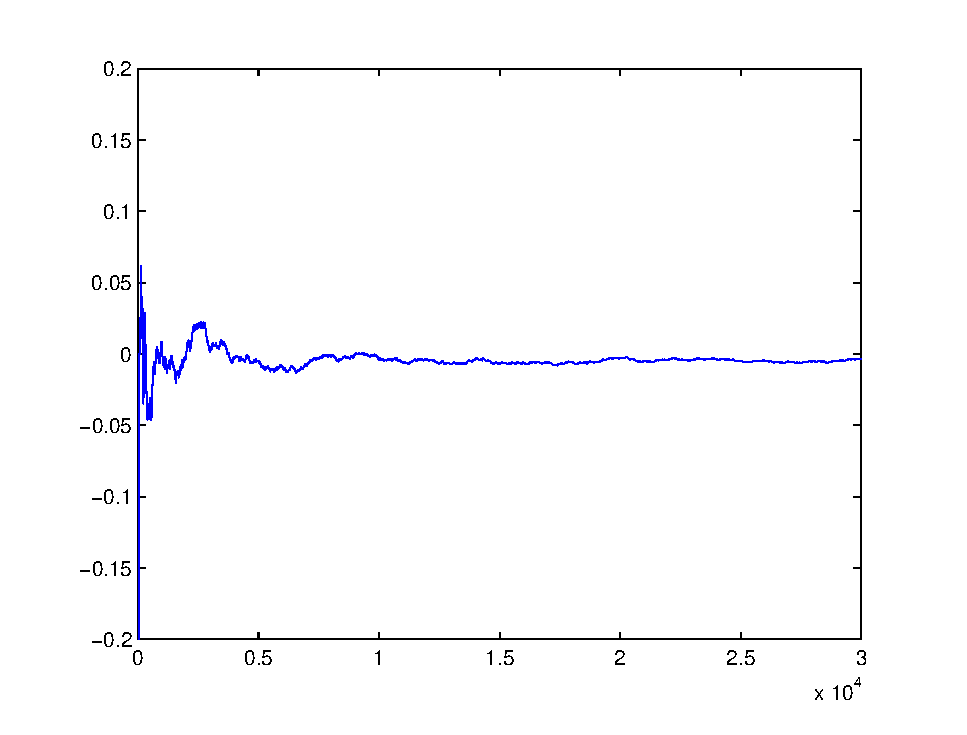
\includegraphics[scale=0.34]{images/balance_oldci_xx.eps}
} \hspace{0.5cm}
\subfigure[Old CI(ISAAC, XORshift)]{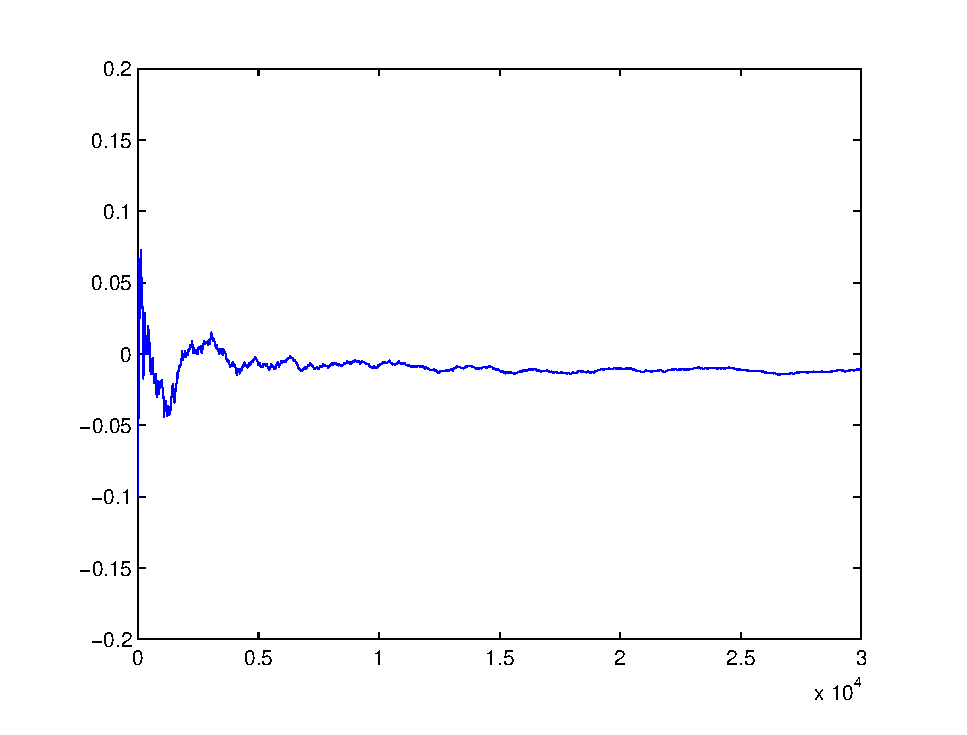
\includegraphics[scale=0.34]{images/balance_oldci_xi.eps}
} \hspace{0.5cm}
\subfigure[Old CI(ISAAC, ISAAC)]{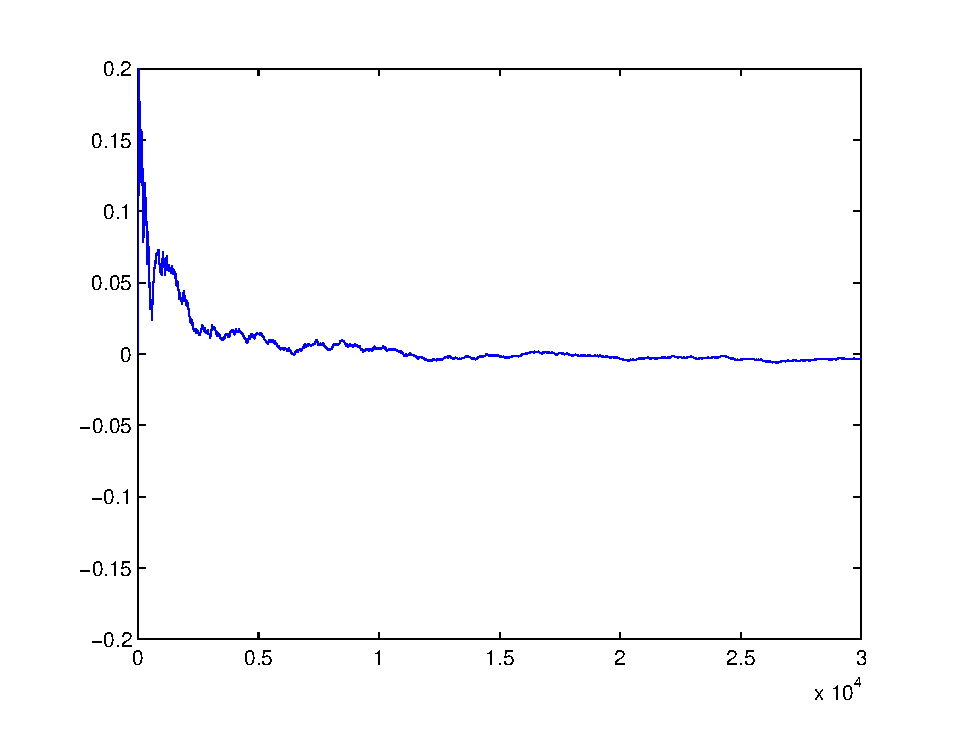
\includegraphics[scale=0.34]{images/balance_oldci_ii.eps}
} \hspace{0.5cm}
\caption{Balance of Probability for old CI}
\label{Balance of Probability for old CI}
\end{figure}

\begin{figure}
\centering
\subfigure[New CI(XORshift, XORshift)]{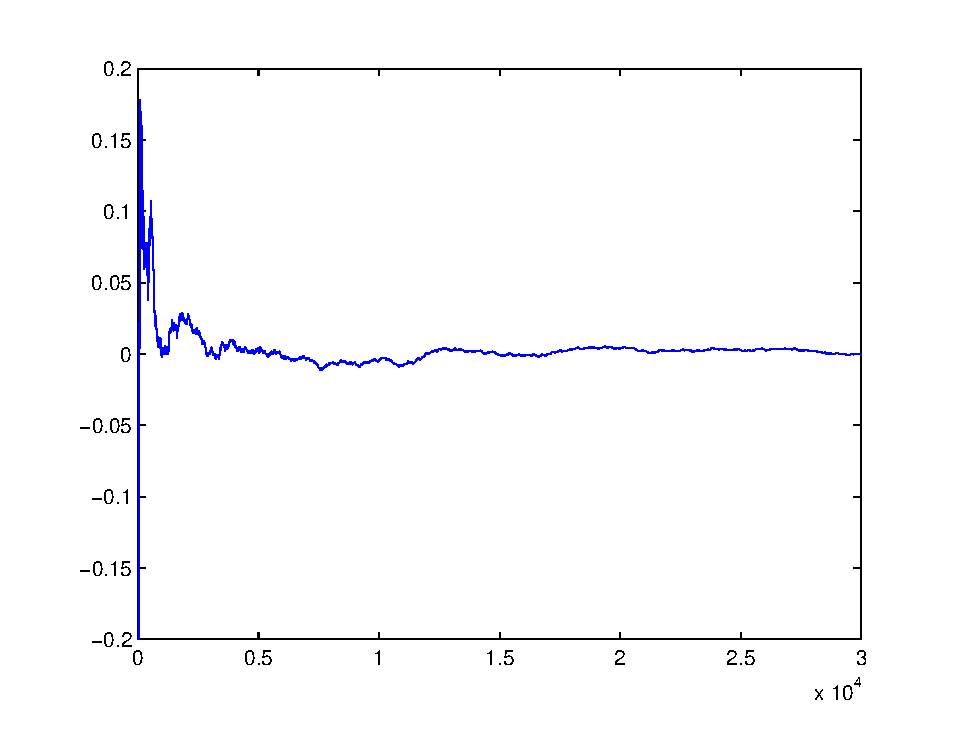
\includegraphics[scale=0.34]{images/balance_newci_xx.eps}
} \hspace{0.5cm}
\subfigure[New CI(ISAAC, XORshift)]{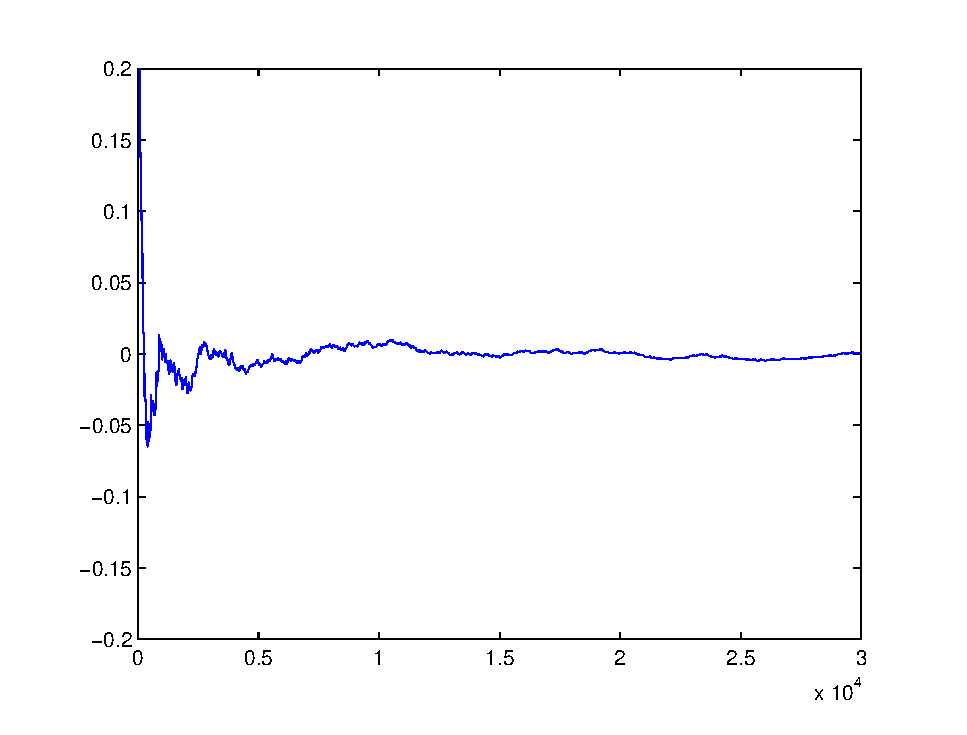
\includegraphics[scale=0.34]{images/balance_newci_xi.eps}
} \hspace{0.5cm}
\subfigure[New CI(ISAAC, ISAAC)]{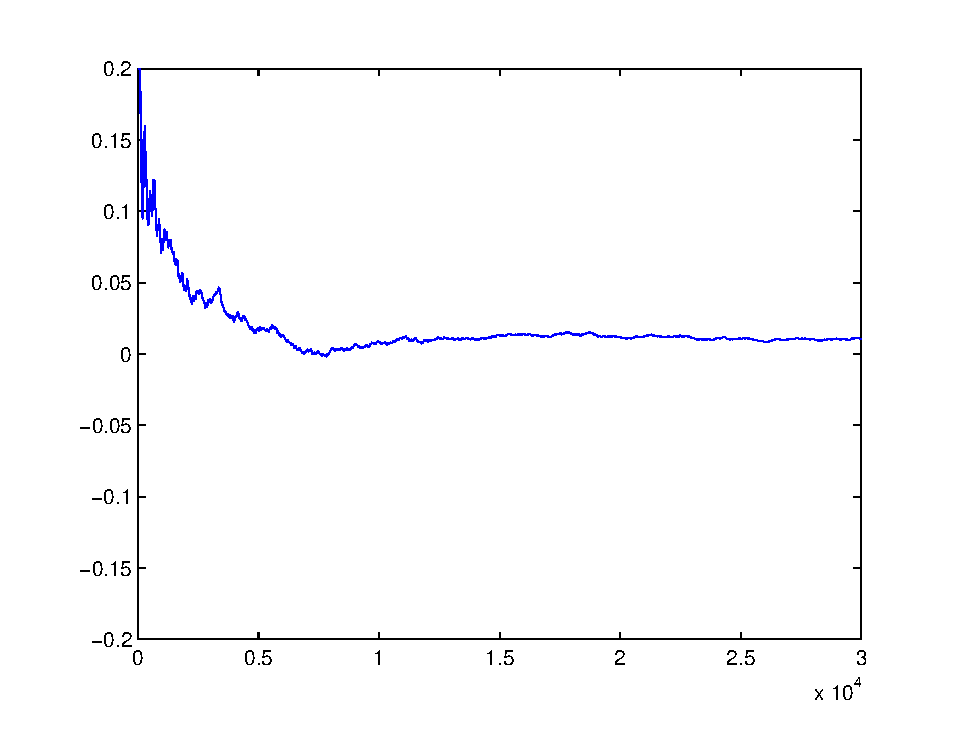
\includegraphics[scale=0.34]{images/balance_newci_ii.eps}
} \hspace{0.5cm}
\caption{Balance of Probability for new CI}
\label{Balance of Probability for new CI}
\end{figure}

\section{Sensitivity}

As a consequence of its chaotic property, this PRNG is highly sensitive to the initial conditions. To illustrate this property, several initial values are put into the chaotic system. Let $H$ be the number 
of differences between the sequences obtained in this way. Suppose $n$ is the length of these 
sequences. Then the variance ratio $P$, defined by $P = H / n$, is computed. The results are 
shown in Figure~\ref{Sensitivity for old CI} and Figure~\ref{Sensitivity for new CI} ($x$ axis is sequence lengths, $y$ axis is variance ratio $P$). For the two PRNGs, variance 
ratios approach $0.50$, which indicate that the systems are extremely sensitive to the initial 
conditions.
\begin{figure}
\centering
\subfigure[Old CI(Logistic, Logistic)]{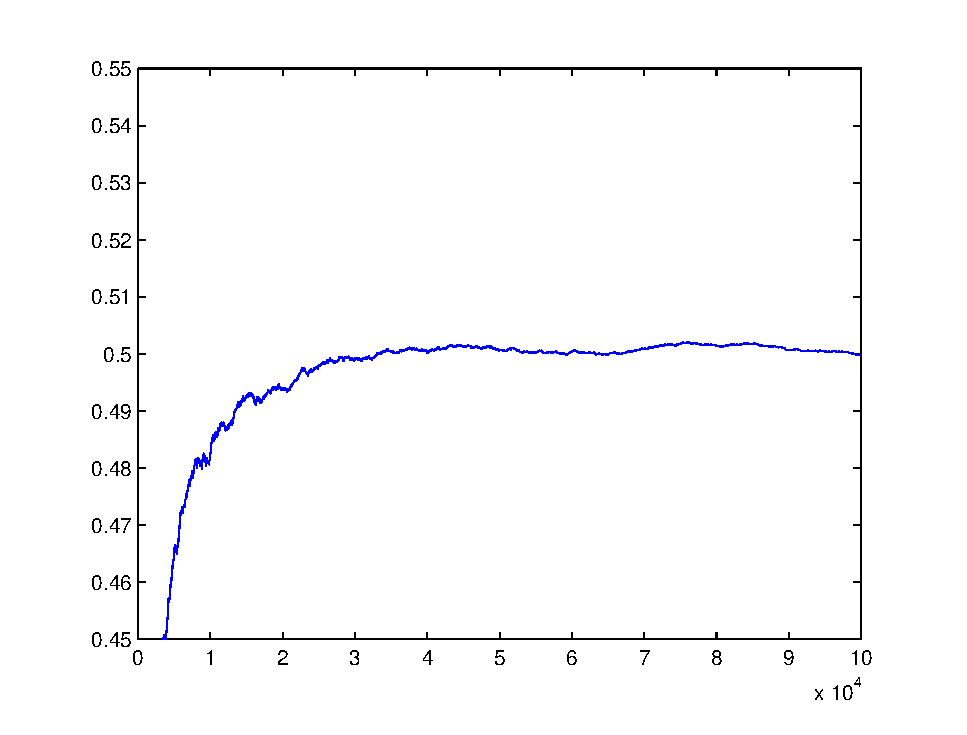
\includegraphics[scale=0.34]{images/Sensitivity_oldci_ll.eps}
} \hspace{0.5cm}
\subfigure[Old CI(XORshift, XORshift)]{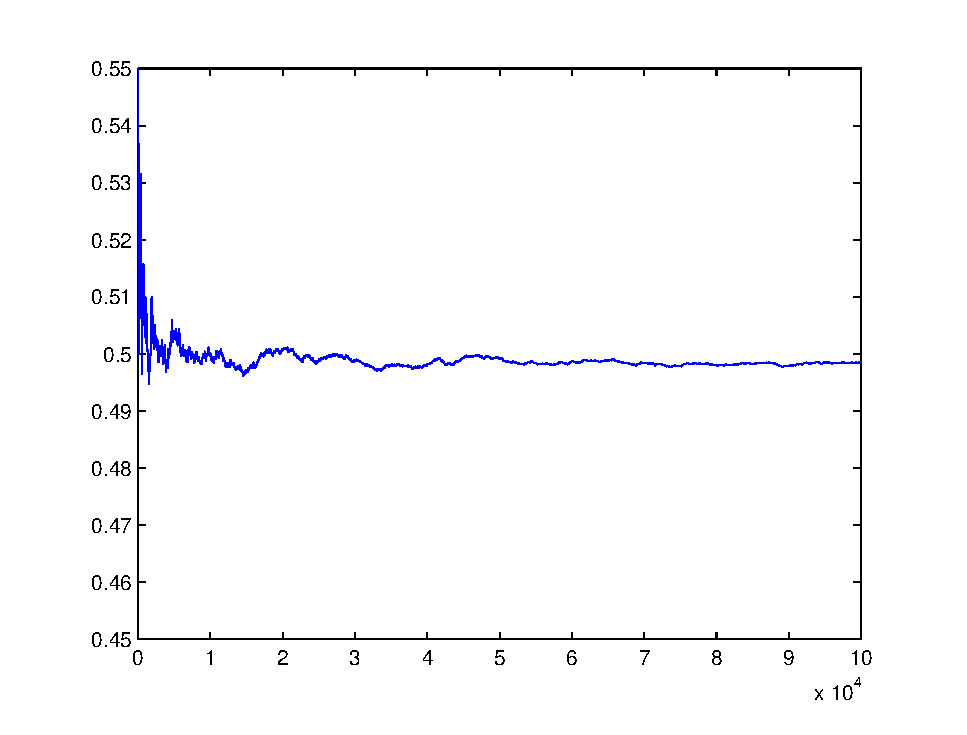
\includegraphics[scale=0.34]{images/Sensitivity_oldci_xx.eps}
} \hspace{0.5cm}
\subfigure[Old CI(ISAAC, XORshift)]{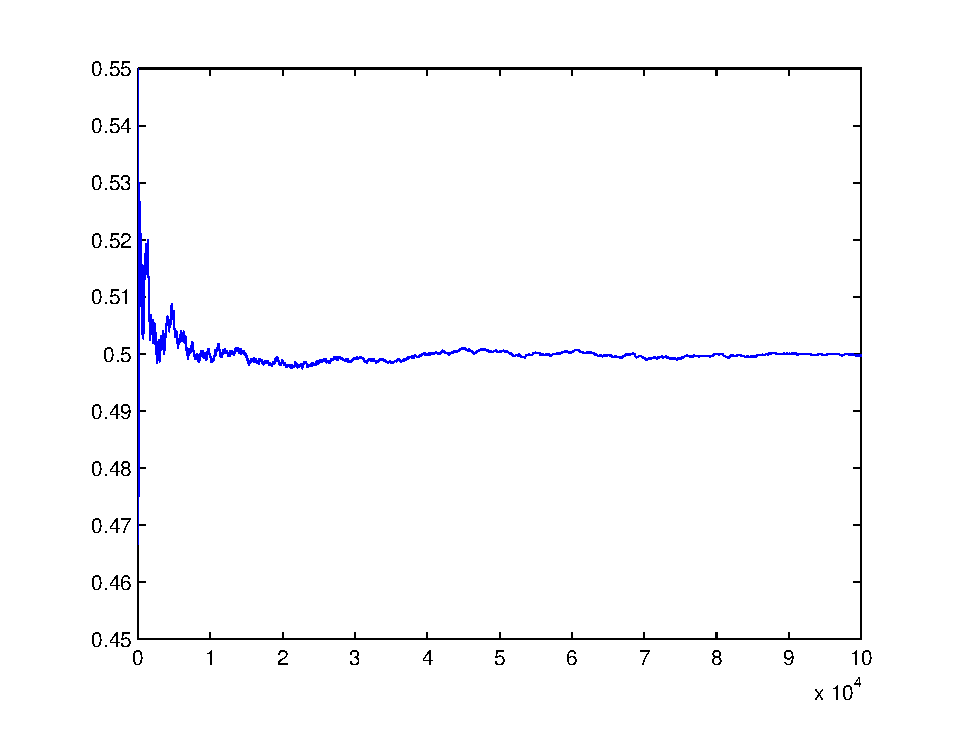
\includegraphics[scale=0.34]{images/Sensitivity_oldci_xi.eps}
} \hspace{0.5cm}
\subfigure[Old CI(ISAAC, ISAAC)]{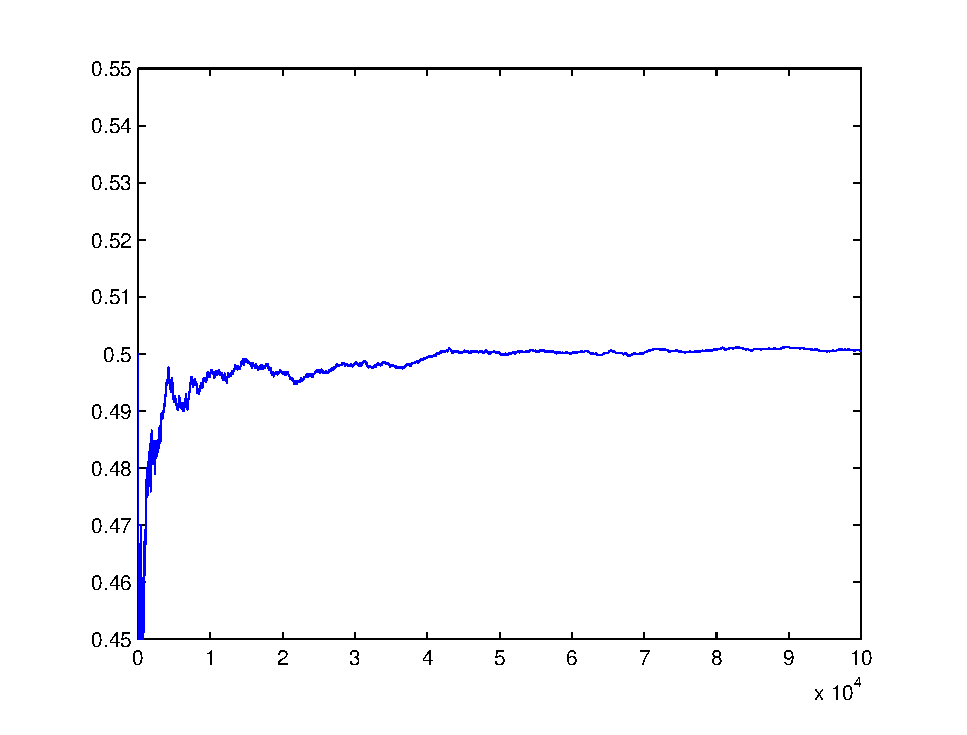
\includegraphics[scale=0.34]{images/Sensitivity_oldci_ii.eps}
} \hspace{0.5cm}
\caption{Sensitivity for old CI}
\label{Sensitivity for old CI}
\end{figure}

\begin{figure}
\centering
\subfigure[New CI(XORshift, XORshift)]{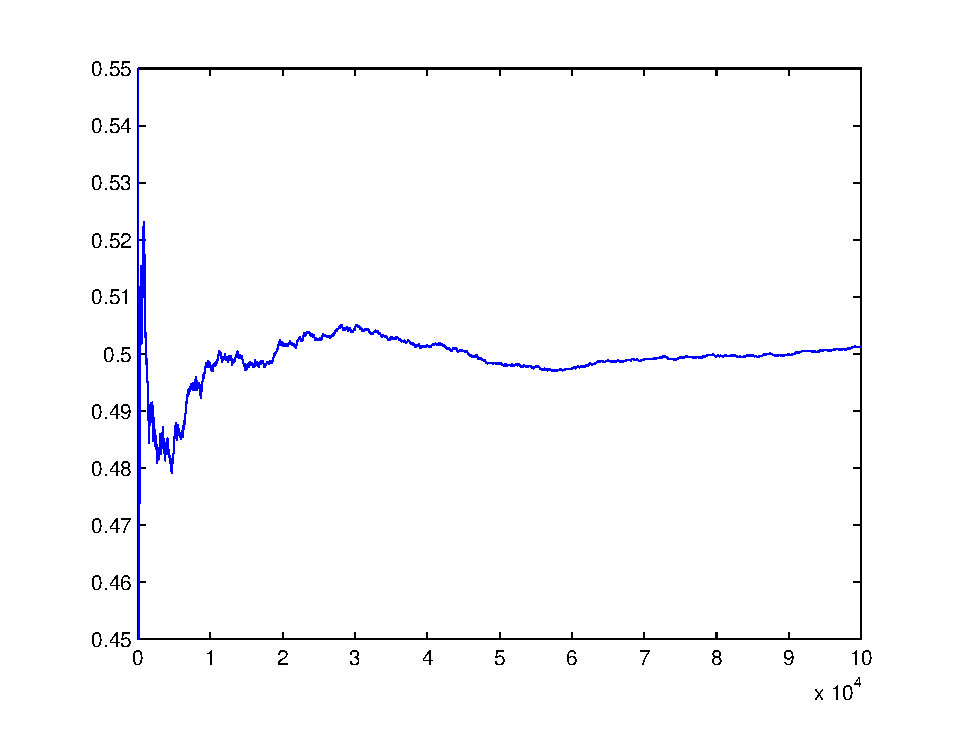
\includegraphics[scale=0.34]{images/Sensitivity_newci_xx.eps}
} \hspace{0.5cm}
\subfigure[New CI(ISAAC, XORshift)]{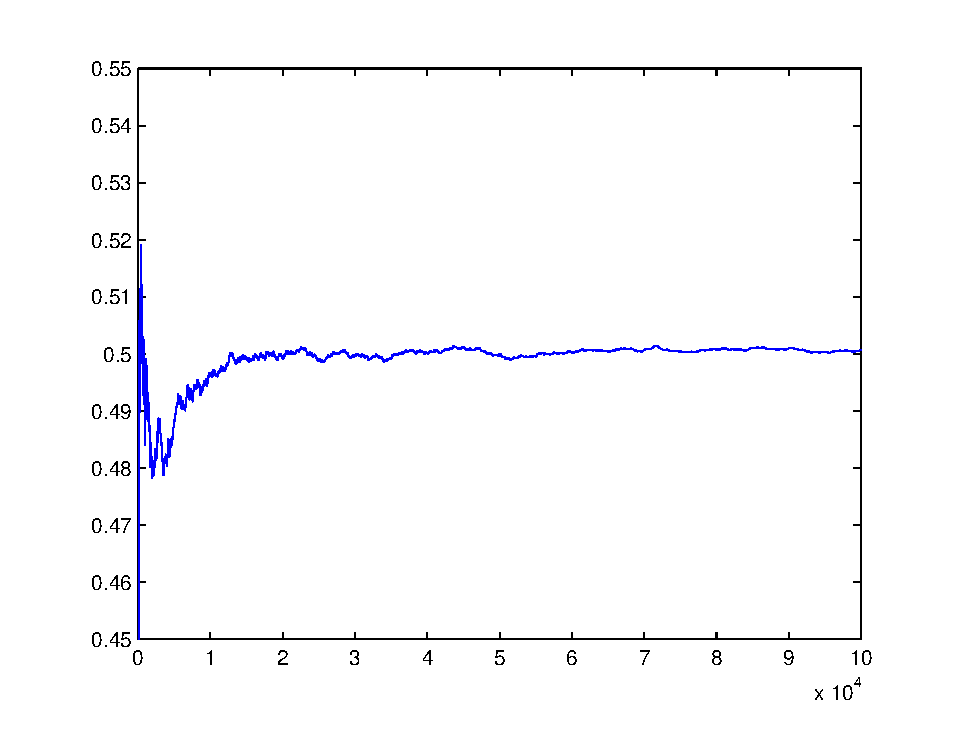
\includegraphics[scale=0.34]{images/Sensitivity_newci_xi.eps}
} \hspace{0.5cm}
\subfigure[New CI(ISAAC, ISAAC)]{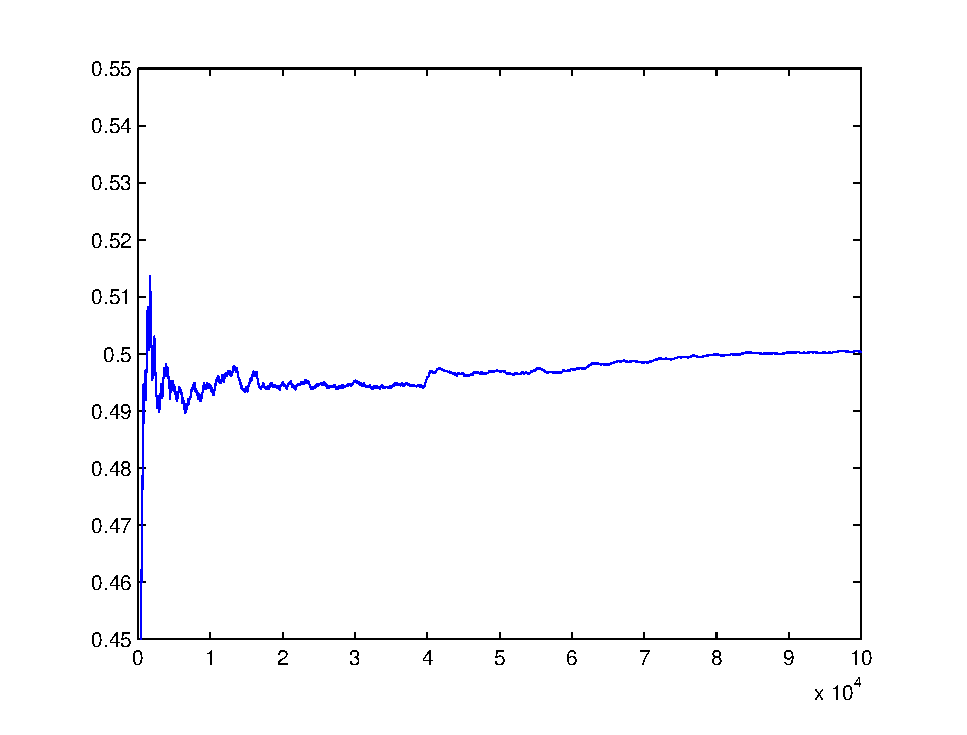
\includegraphics[scale=0.34]{images/Sensitivity_newci_ii.eps}
} \hspace{0.5cm}
\caption{Sensitivity for new CI}
\label{Sensitivity for new CI}
\end{figure}


\section{Pattern}
If a sequence consists of periodic features or repetitive patterns, it is not random [58]. These data patterns existed in the sequence can be revealed by the use of recurrence plot [59], which can be constructed as follows.

Considering a sequence ${x_0,x_1\ldots x_n}$, a vector $y_i$ of dimension $m\geqslant2$ and delay $d\geqslant1$ can be constructed by:
\begin{equation}
\centering
y_i=(x_i,x_{i+d},x_{i+2d},\ldots,x_{i+(m-1)d})
\end{equation}
The recurrence plot is then obtained by plotting a point if the following condition is satisfied:
\begin{equation}
\centering
||y_j-y_i||<t
\end{equation}
where t is a threshold distance.

Figure~\ref{The corresponding recurrence plot for old CI} and Figure~\ref{The corresponding recurrence plot for new CI} depict some sampled  recurrence plots with $m=2$, $d=1$, $t=0.05$, respectively. The points are scattered as shown in Figures, patterns can not easily observed as it is non-periodic and random.
\begin{figure}
\centering
\subfigure[Old CI(Logistic, Logistic)]{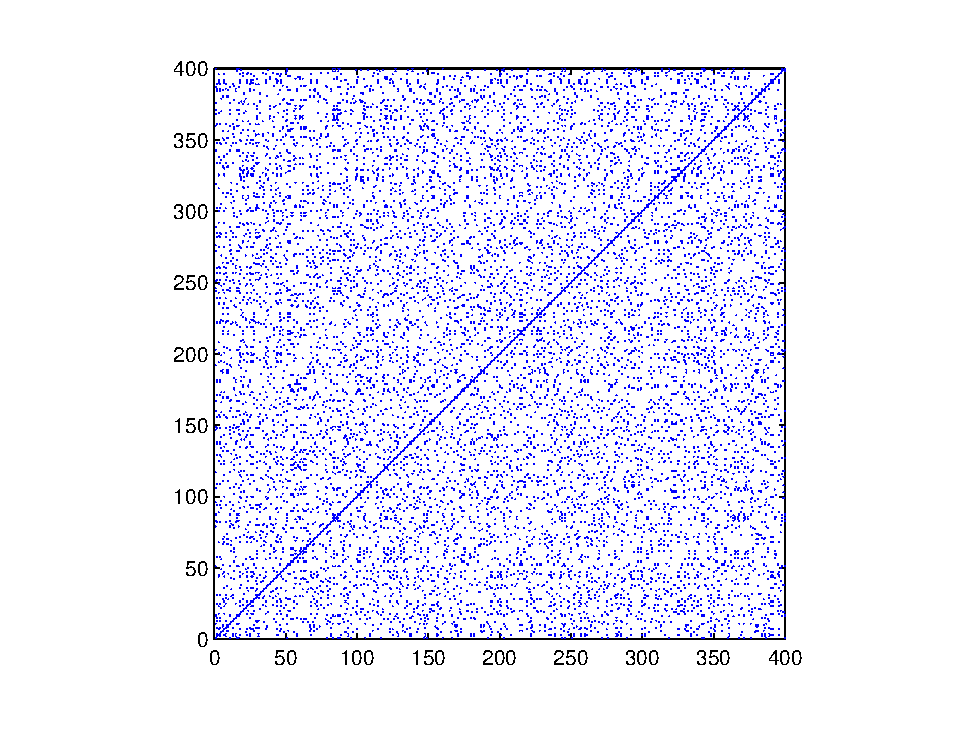
\includegraphics[scale=0.4]{images/pattern_oldci_ll.eps}
} \hspace{0.5cm}
\subfigure[Old CI(XORshift, XORshift)]{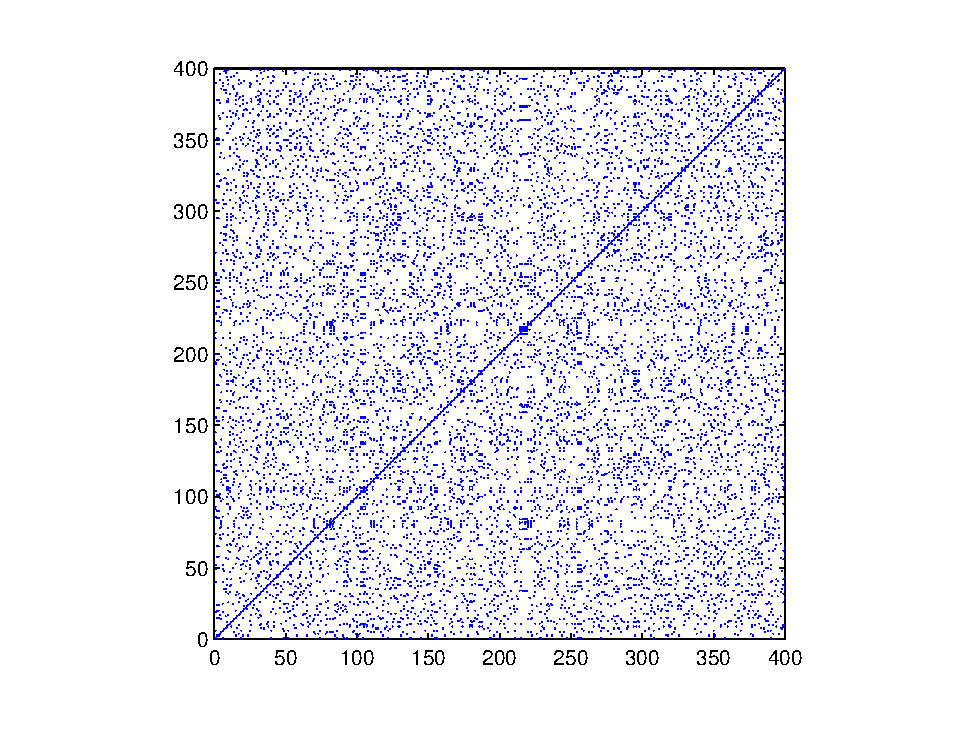
\includegraphics[scale=0.4]{images/pattern_oldci_xx.eps}
} \hspace{0.5cm}
\subfigure[Old CI(ISAAC, XORshift)]{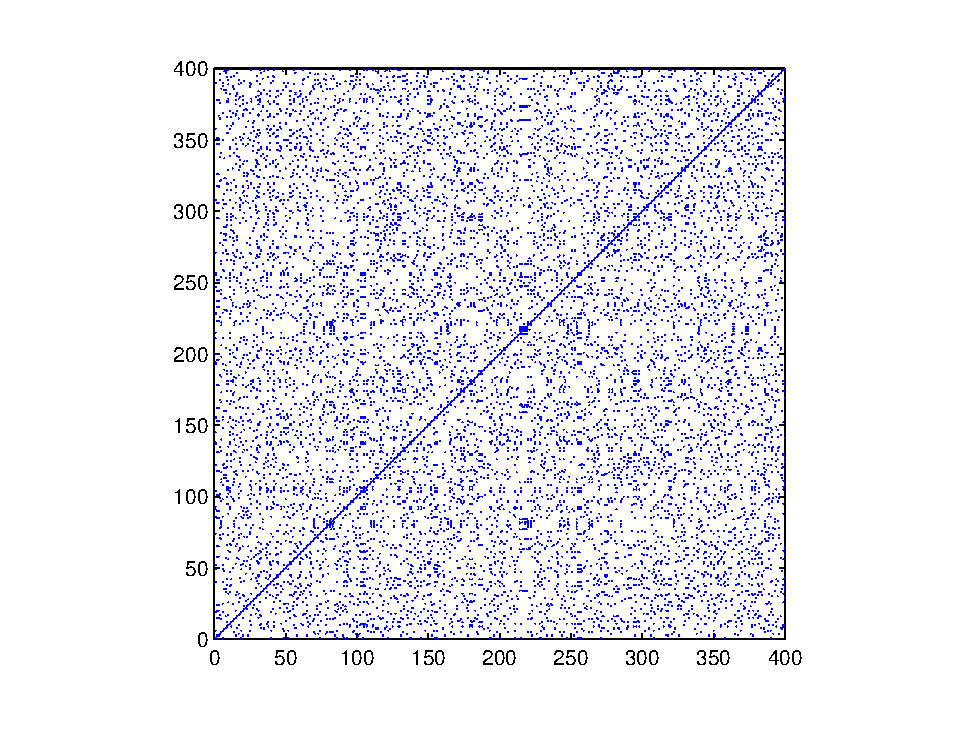
\includegraphics[scale=0.4]{images/pattern_oldci_xi.eps}
} \hspace{0.5cm}
\subfigure[Old CI(ISAAC, ISAAC)]{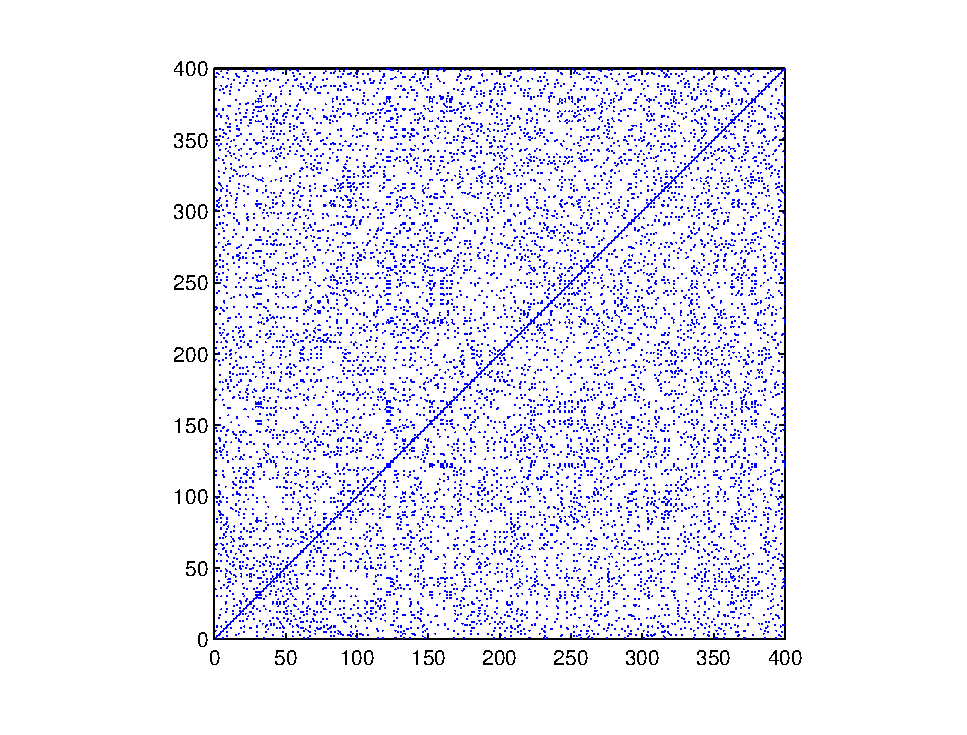
\includegraphics[scale=0.4]{images/pattern_oldci_ii.eps}
} \hspace{0.5cm}
\caption{The corresponding recurrence plot for old CI}
\label{The corresponding recurrence plot for old CI}
\end{figure}

\begin{figure}
\centering
\subfigure[New CI(XORshift, XORshift)]{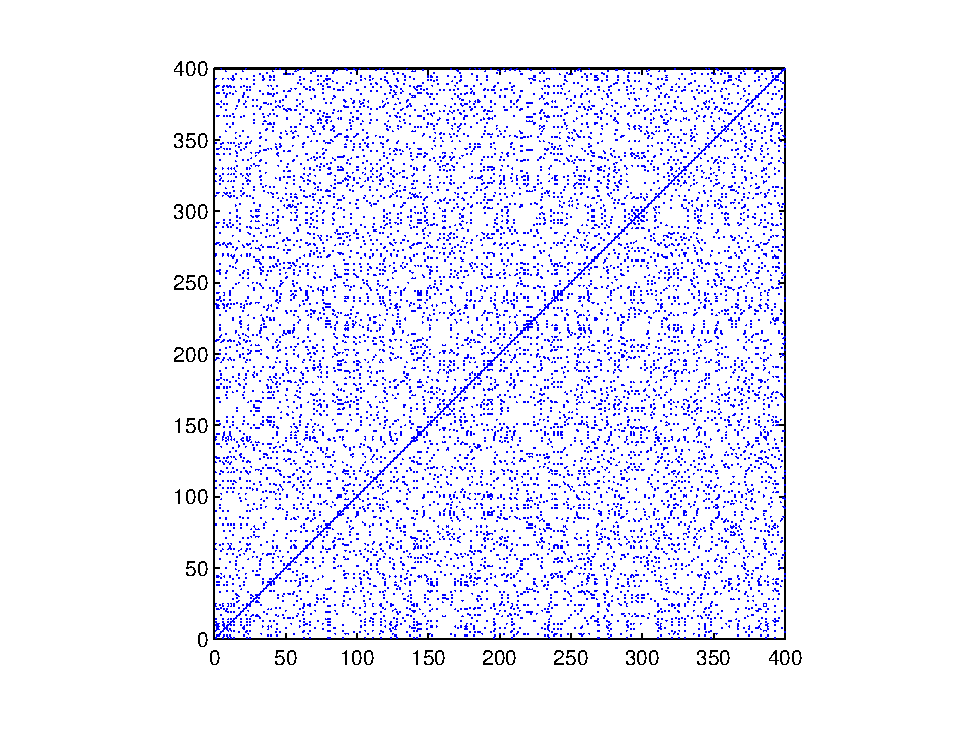
\includegraphics[scale=0.41]{images/pattern_newci_xx.eps}
} \hspace{0.5cm}
\subfigure[New CI(ISAAC, XORshift)]{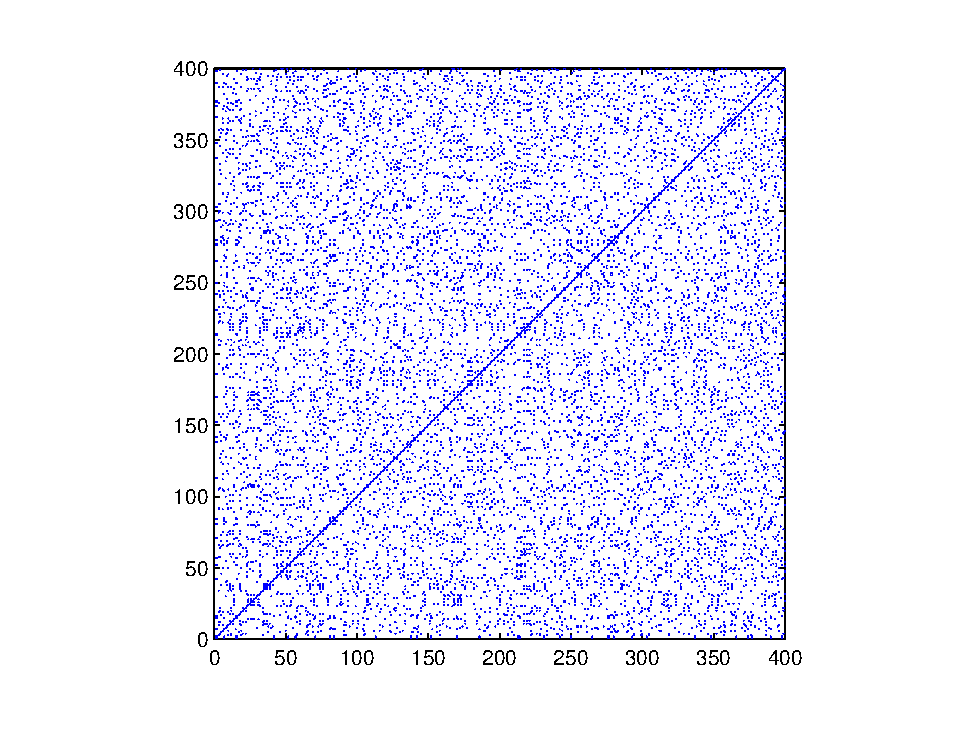
\includegraphics[scale=0.4]{images/pattern_newci_xi.eps}
} \hspace{0.5cm}
\subfigure[New CI(ISAAC, ISAAC)]{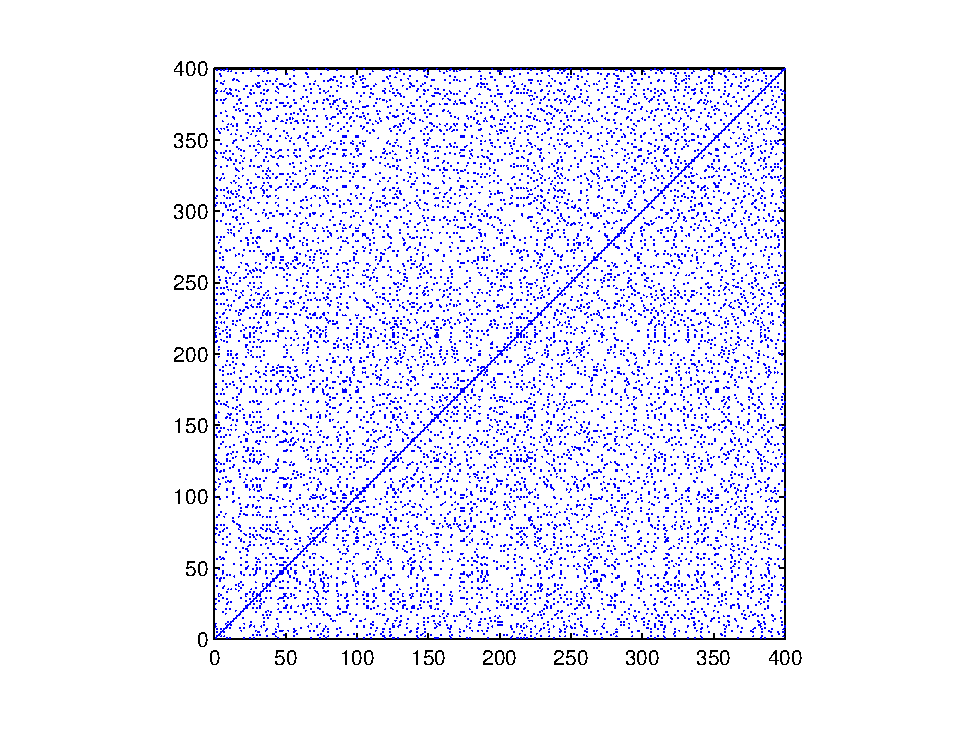
\includegraphics[scale=0.4]{images/pattern_newci_ii.eps}
} \hspace{0.5cm}
\caption{The corresponding recurrence plot for new CI}
\label{The corresponding recurrence plot for new CI}
\end{figure}


\section{Linear complexity}
A sequence is considered to be random only if it cannot be
reconstructed with a short program, or cannot be described by some simple laws. Therefore, if
a sequence is random, it has maximal complexity [60], and data compression is nearly
impossible.

The linear complexity (LC) of a sequence is the size in bits of the shortest linear feedback shift register (LFSR) which can produce this sequence. This value measures the difficulty of generating -- and perhaps analyzing -- a particular sequence.
Indeed, the randomness of a given sequence can be linked to the size of the smallest program that can produce it. LC is the size required by a LFSR to be able to produce the given sequence. The Berlekamp-Massey algorithm can measure this LC, which might be used to evaluate the ``security'' of a pseudo-random sequence.

It can be seen in Figure~\ref{Linear complexity for old CI} and Figure~\ref{Linear complexity for new CI} that the LC curves of sample sequences of 2000 b are close to the ideal line $C_i=i/2$, which imply that the generator has high linear complexity. 
\begin{figure}
\centering
\subfigure[Old CI(Logistic, Logistic)]{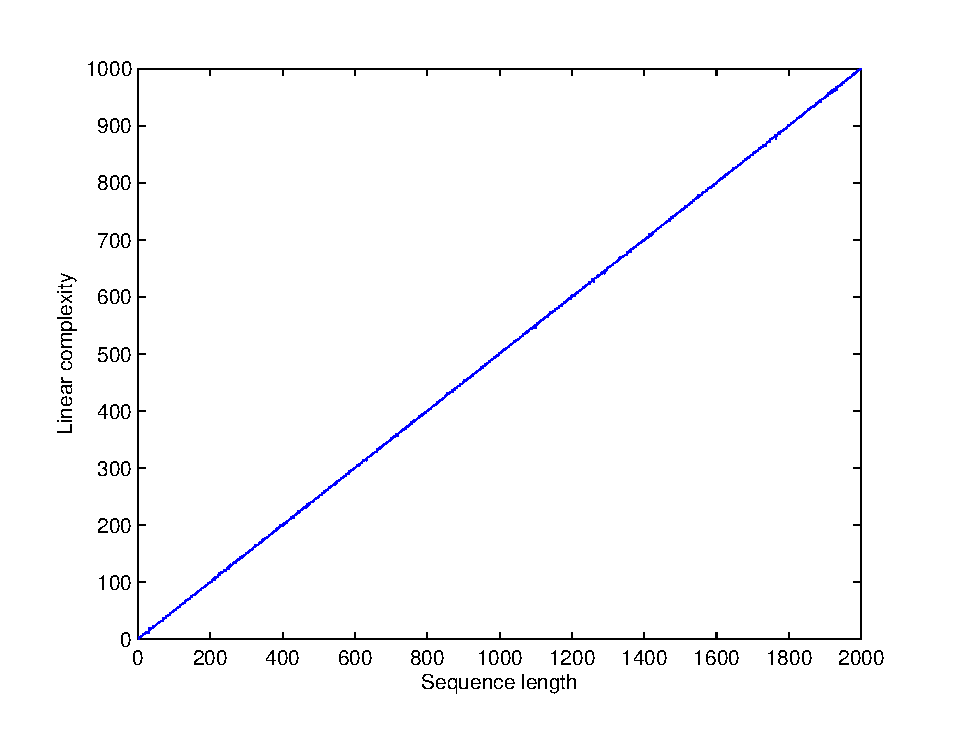
\includegraphics[scale=0.34]{images/linear_complexity_oldci_ll.eps}
} \hspace{0.5cm}
\subfigure[Old CI(XORshift, XORshift)]{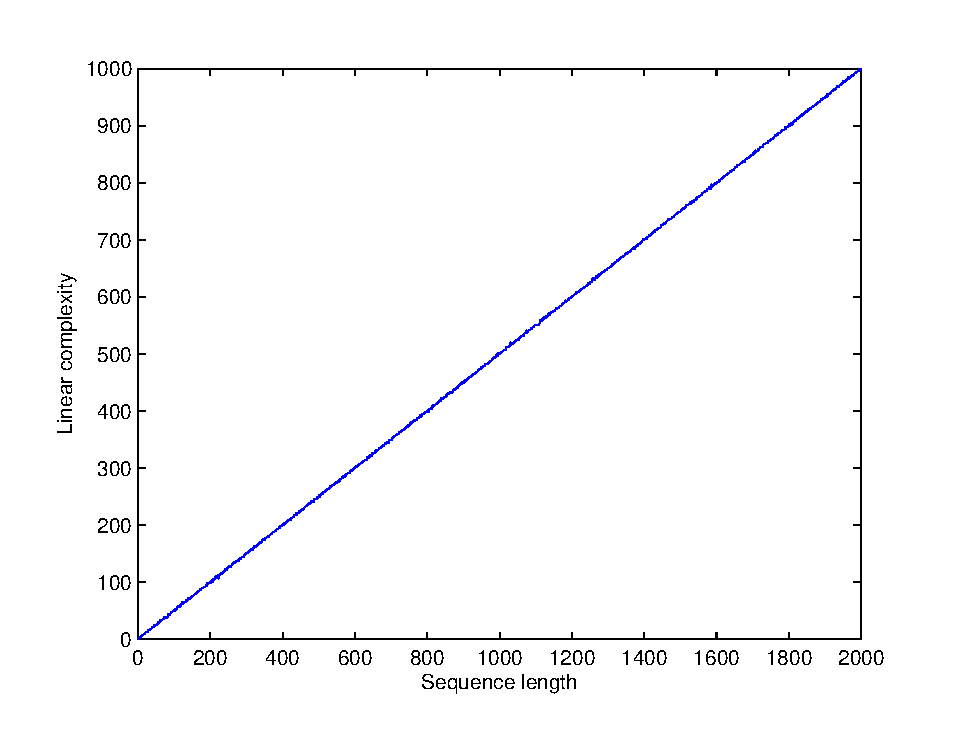
\includegraphics[scale=0.34]{images/linear_complexity_oldci_xx.eps}
} \hspace{0.5cm}
\subfigure[Old CI(ISAAC, XORshift)]{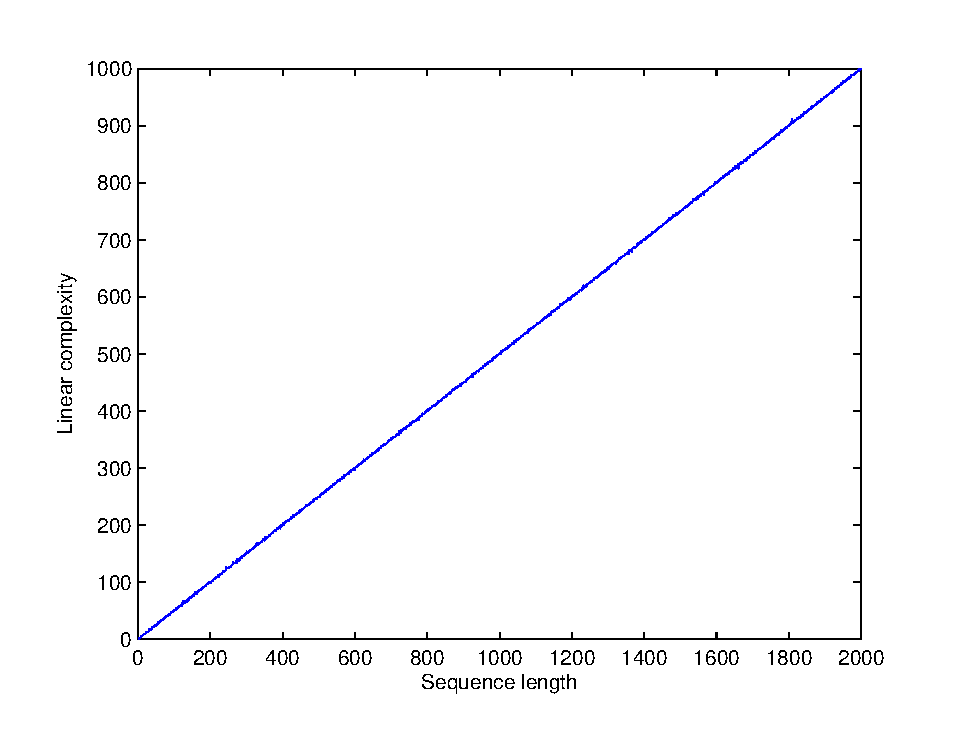
\includegraphics[scale=0.34]{images/linear_complexity_oldci_xi.eps}
} \hspace{0.5cm}
\subfigure[Old CI(ISAAC, ISAAC)]{\includegraphics[scale=0.34]{images/linear_complexity_oldci_ii.eps}
} \hspace{0.5cm}
\caption{Linear complexity for old CI}
\label{Linear complexity for old CI}
\end{figure}

\begin{figure}
\centering
\subfigure[New CI(XORshift, XORshift)]{\includegraphics[scale=0.34]{images/linear_complexity_newci_xx.eps}
} \hspace{0.5cm}
\subfigure[New CI(ISAAC, XORshift)]{\includegraphics[scale=0.34]{images/linear_complexity_newci_xi.eps}
} \hspace{0.5cm}
\subfigure[New CI(ISAAC, ISAAC)]{\includegraphics[scale=0.34]{images/linear_complexity_newci_ii.eps}
} \hspace{0.5cm}
\caption{Linear complexity for new CI}
\label{Linear complexity for new CI}
\end{figure}


\section{Uniform distribution}

Figure~\ref{Second order distribution for old CI} and Figure~\ref{Second order distribution for new CI} give a 3D graphic representation of the distribution of a random sequence obtained by our generators. The point cloud presents a uniform distribution that tends to fill the complete 3D space, as expected for a random signal. To obtain this cloud, we have first changed the binary sequence to a $N$-bit integer sequence $x_1$, $x_2$, $x_3$, $x_4$... Then we have plot $\left(\frac{x_1}{2^N},\frac{x_2}{2^N},\frac{x_3}{2^N}\right), \left(\frac{x_2}{2^N},\frac{x_3}{2^N},\frac{x_4}{2^N}\right)$...

\begin{figure}
\centering
\subfigure[Old CI(Logistic, Logistic)]{\includegraphics[scale=0.34]{images/distribution_oldci_ll.eps}
} \hspace{0.5cm}
\subfigure[Old CI(XORshift, XORshift)]{\includegraphics[scale=0.34]{images/distribution_oldci_xx.eps}
\label{Old CI(XORshift, XORshift)}} \hspace{0.5cm}
\subfigure[Old CI(ISAAC, XORshift)]{\includegraphics[scale=0.34]{images/distribution_oldci_xi.eps}
\label{Old CI(ISAAC, XORshift)}} \hspace{0.5cm}
\subfigure[Old CI(ISAAC, ISAAC)]{\includegraphics[scale=0.34]{images/distribution_oldci_ii.eps}
\label{Old CI(ISAAC, ISAAC)}} \hspace{0.5cm}
\caption{Second order distribution for old CI}
\label{Second order distribution for old CI}
\end{figure}

\begin{figure}
\centering
\subfigure[New CI(XORshift, XORshift)]{\includegraphics[scale=0.34]{images/distribution_newci_xx.eps}
} \hspace{0.5cm}
\subfigure[New CI(ISAAC, XORshift)]{\includegraphics[scale=0.34]{images/distribution_newci_xi.eps}
} \hspace{0.5cm}
\subfigure[New CI(ISAAC, ISAAC)]{\includegraphics[scale=0.34]{images/distribution_newci_ii.eps}
} \hspace{0.5cm}
\caption{Second order distribution for new CI}
\label{Second order distribution for new CI}
\end{figure}


\section{Auto-correlation and cross-correlation}
Since the number in a random sequence should be unpredictable and hence uncorrelated,
the auto-correlation and the cross-correlation between sequences can also be used to reflect
the randomness of a sequence. These correlation values are also the prime indices when a
random sequence is to be used in spread-spectrum communications [57].

Let $\{u\}$ and $\{v\}$ be two binary $(-1,+1)$-value sequences of length $n$, the aperiodic
auto-correlation function $C_{uu}(l)$ and the aperiodic cross-correlation function $C_{uv}(l)$ are defined
in Equation (\ref{auto}) and (\ref{cross}), respectively.
\begin{equation}
\label{auto}
C_{u,u}(l)=
\left\{
\begin{array}{llc}
\sum_{i=0}^{n-1-l} u_{i}u_{i+l} & \text{ if }&0\leqslant l\leqslant n-1\\
\sum_{i=0}^{n-1+l} u_{i-l}u_{i}  & \text{ if }&1-n\leqslant l\leqslant 0 \\
0 & \text{ if }&|l|\geqslant n\\
\end{array}
\right.
\end{equation}
\begin{equation}
\label{cross}
C_{u,v}(l)=
\left\{
\begin{array}{llc}
\sum_{i=0}^{n-1-l} u_{i}v_{i+l} & \text{ if }&0\leqslant l\leqslant n-1\\
\sum_{i=0}^{n-1+l} u_{i-l}v_{i}  & \text{ if }&1-n\leqslant l\leqslant 0 \\
0 & \text{ if }&|l|\geqslant n\\
\end{array}
\right.
\end{equation}


The auto-correlation and cross-correlation of the symbolic sequences are respectively given in Figure.~\ref{autocorr for old CI}, Figure.~\ref{autocorr for new CI}, Figure.~\ref{intercorr for old CI} and Figure.~\ref{intercorr for new CI}demonstrating a nice nature. It can be seen that this sequences have $\delta$-like auto-correlation which is required for a good PRBNG. The sequences generated with different initial values will have zero cross-correlation due to the sensitive dependence on initial conditions. 



\begin{figure}
\centering
\subfigure[Old CI(Logistic, Logistic)]{\includegraphics[scale=0.34]{images/autocorr_oldci_ll.eps}
} \hspace{0.5cm}
\subfigure[Old CI(XORshift, XORshift)]{\includegraphics[scale=0.34]{images/autocorr_oldci_xx.eps}
} \hspace{0.5cm}
\subfigure[Old CI(ISAAC, XORshift)]{\includegraphics[scale=0.34]{images/autocorr_oldci_xi.eps}
} \hspace{0.5cm}
\subfigure[Old CI(ISAAC, ISAAC)]{\includegraphics[scale=0.34]{images/autocorr_oldci_ii.eps}
} \hspace{0.5cm}
\caption{Auto-correlation for old CI}
\label{autocorr for old CI}
\end{figure}

\begin{figure}
\centering
\subfigure[New CI(XORshift, XORshift)]{\includegraphics[scale=0.34]{images/autocorr_newci_xx.eps}
} \hspace{0.5cm}
\subfigure[New CI(ISAAC, XORshift)]{\includegraphics[scale=0.34]{images/autocorr_newci_xi.eps}
} \hspace{0.5cm}
\subfigure[New CI(ISAAC, ISAAC)]{\includegraphics[scale=0.34]{images/autocorr_newci_ii.eps}
} \hspace{0.5cm}
\caption{Auto-correlation for new CI}
\label{autocorr for new CI}
\end{figure}

\begin{figure}
\centering
\subfigure[Old CI(Logistic, Logistic)]{\includegraphics[scale=0.34]{images/intercorr_oldci_ll.eps}
} \hspace{0.5cm}
\subfigure[Old CI(XORshift, XORshift)]{\includegraphics[scale=0.34]{images/intercorr_oldci_xx.eps}
} \hspace{0.5cm}
\subfigure[Old CI(ISAAC, XORshift)]{\includegraphics[scale=0.34]{images/intercorr_oldci_xi.eps}
} \hspace{0.5cm}
\subfigure[Old CI(ISAAC, ISAAC)]{\includegraphics[scale=0.34]{images/intercorr_newci_ii.eps}
} \hspace{0.5cm}
\caption{Cross-correlation for old CI}
\label{intercorr for old CI}
\end{figure}

\begin{figure}
\centering
\subfigure[New CI(XORshift, XORshift)]{\includegraphics[scale=0.34]{images/intercorr_newci_xx.eps}
} \hspace{0.5cm}
\subfigure[New CI(ISAAC, XORshift)]{\includegraphics[scale=0.34]{images/intercorr_newci_xi.eps}
} \hspace{0.5cm}
\subfigure[New CI(ISAAC, ISAAC)]{\includegraphics[scale=0.34]{images/intercorr_newci_ii.eps}
} \hspace{0.5cm}
\caption{Cross-correlation for new CI}
\label{intercorr for new CI}
\end{figure}
\section{FFT}

The FFT of the sequences (Figure.~\ref{FFT for old CI} and Figure.~\ref{FFT for new CI}) are performed and the corresponding power spectrums are computed. Some complete flat power spectrums, with almost equal frequency contribution for all frequencies, are indicative of a total random series.

\begin{figure}
\centering
\subfigure[Old CI(Logistic, Logistic)]{\includegraphics[scale=0.34]{images/fft_oldci_ll.eps}
} \hspace{0.5cm}
\subfigure[Old CI(XORshift, XORshift)]{\includegraphics[scale=0.34]{images/fft_oldci_xx.eps}
} \hspace{0.5cm}
\subfigure[Old CI(ISAAC, XORshift)]{\includegraphics[scale=0.34]{images/fft_oldci_xi.eps}
} \hspace{0.5cm}
\subfigure[Old CI(ISAAC, ISAAC)]{\includegraphics[scale=0.34]{images/fft_oldci_ii.eps}
} \hspace{0.5cm}
\caption{FFT for old CI}
\label{FFT for old CI}
\end{figure}

\begin{figure}
\centering
\subfigure[New CI(XORshift, XORshift)]{\includegraphics[scale=0.34]{images/fft_newci_xx.eps}
} \hspace{0.5cm}
\subfigure[New CI(ISAAC, XORshift)]{\includegraphics[scale=0.34]{images/fft_newci_xi.eps}
} \hspace{0.5cm}
\subfigure[New CI(ISAAC, ISAAC)]{\includegraphics[scale=0.34]{images/fft_newci_ii.eps}
} \hspace{0.5cm}
\caption{FFT for new CI}
\label{FFT for new CI}
\end{figure}

\section{Devaney's Chaos Property}

Generally speaking, the quality of a PRNG depends, to a large extent, on the following criteria: randomness, uniformity, independence, storage efficiency, and reproducibility. A chaotic sequence may satisfy these requirements and also other chaotic properties, as ergodicity, entropy, and expansivity. A chaotic sequence is extremely sensitive to the initial conditions. That is, even a minute difference in the initial state of the system can lead to enormous differences in the final state, even over fairly small timescales. Therefore, chaotic sequence fits the requirements of pseudo-random sequence well. Contrary to XORshift and ISAAC, our generator possesses these chaotic properties~\cite{guyeux09},\cite{wang2009}.
However, despite a large number of papers published in the field of chaos-based pseudo-random generators, the impact of this research is rather marginal. This is due to the following reasons: almost all PRNG algorithms using chaos are based on dynamical systems defined on continuous sets (\emph{e.g.}, the set of real numbers). So these generators are usually slow, requiring considerably more storage space, and lose their chaotic properties during computations as mentioned earlier in this paper. These major problems restrict their use as generators~\cite{Kocarev2001}.

In this paper we do not simply integrate chaotic maps hoping that the implemented algorithm remains chaotic. Indeed, the PRNGs we conceive are just discrete chaotic iterations and we have proven in \cite{guyeux09} that these iterations produce a topological chaos as defined by Devaney: they are regular, transitive, and sensitive to initial conditions. This famous definition of a chaotic behavior for a dynamical system implies unpredictability, mixture, sensitivity, and uniform repartition. Moreover, as only integers are manipulated in discrete chaotic iterations, the chaotic behavior of the system is preserved during computations, and these computations are fast.

Let us now explore the topological properties of our generator and their consequences concerning the quality of the generated pseudo-random sequences.
%Generally speaking, the success of a PRNG study depends, to a large extent, on the following criteria:
%uniformity, independence, storage efficiency, reproducibility. Chaotic sequence
%has not only these good pseudo-random characteristics but also chaotic properties,
%as ergodicity, entropy and expansivity. It is extremely sensitive to the initial states. That is, even a minute
%difference in the starting state of the
%system can lead to enormous differences in the final state of the system even over
%fairly small timescales. Therefore, chaotic sequence well fits the requirements of
%pseudo-random sequence.\newline
%Despite a huge number of papers published in the field of chaos-based pseudo-random generators, the impact that this research has made on conventional cryptography is rather marginal. This is due to the following reasons: almost all chaotic algorithms are based on dynamical systems defined on the set of real numbers. So these generators are usually slow, require considerably more storage space and lose their chaotic property during computations. These major problems restrict their use in cryptography~\cite{Kocarev2001}.\newline
%The generator proposed in this paper does not inherit its chaotic properties from a real chaotic map, but from chaotic iterations defined in Section \ref{subsection:Chaotic iterations}. It has been proved in~\cite{guyeux09} that chaotic iterations behave as chaos, as it is defined by Devaney: they are regular, transitive and sensitive to initial conditions. This most famous definition of a chaotic behavior for a dynamical system implies unpredictability, mixture, sensitivity
%and uniform repartition. The principal interest is that chaotic iterations don't use real numbers.
%This allows the creation of a new generation of chaotic pseudo-random number generators. Because only integers are manipulated in chaotic iterations, the chaotic behavior of the system is preserved during computations, and these computations are fast.


\section{Topological Consequences}

We have proven in \cite{gfb10:ip} that chaotic iterations are expansive and topologically mixing. These topological properties are inherited by the generators we presented here. In particular, any error on the seed are magnified until being equal to the constant of expansivity.
We will now investigate the consequences of being chaotic, as defined by Devaney. 

First of all, the transitivity property implies the indecomposability of the system:

\begin{definition}
A dynamical system $\left( \mathcal{X}, f\right)$ is indecomposable if it is not the union of two closed sets $A, B \subset \mathcal{X}$ such that $f(A) \subset A, f(B) \subset B$.
\end{definition}

Thus it is impossible to reduce the set of the outputs generated by our PRNG, in order to reduce its complexity. Moreover, it is possible to show that Old and New CI generators are strongly transitive:

\begin{definition}
A dynamical system $\left( \mathcal{X}, f\right)$ is strongly transitive if $\forall x,y \in \mathcal{X},$ $\forall r > 0,$ $\exists z \in \mathcal{X},$ $d(z,x) \leqslant r \Rightarrow$ $\exists n \in \mathds{N}^*,$ $f^n(z)=y$.
\end{definition}

In other words, for all $x,y \in \mathcal{X}$, it is possible to find a point $z$ in the neighborhood of $x$ such that an iterate $f^n(z)$ is $y$. Indeed, this result has been established during the proof of the transitivity presented in~\cite{guyeux09}. Among other things, the strong transitivity property leads to the fact that without the knowledge of the seed, all of the outputs are possible. Additionally, no point of the output space can be discarded when studying our PRNG: it is intrinsically complicated and it cannot be simplified.

Finally, these generators possess the instability property:

\begin{definition}
A dynamical system $\left( \mathcal{X}, f\right)$ is unstable if for all $x \in \mathcal{X}$, the orbit $\gamma_x:n \in \mathds{N} \longmapsto f^n(x)$ is unstable, that is: $\exists \varepsilon > 0,$ $\forall \delta > 0,$ $\exists y \in \mathcal{X},$ $\exists n \in \mathds{N},$ $d(x,y) < \delta$ and $d\left(\gamma_x(n), \gamma_y(n)\right) \geqslant \varepsilon.$
\end{definition}

This property, which is implied by the sensitive dependence to the initial condition, leads to the fact that in all of the neighborhoods of any $x$, there are points which are separate from $x$ under iterations of $f$. We thus can claim that the behavior of our generators is unstable.




\chapter{The family of CIs PRNG}
\label{ThefamilyofCIPRNG}
\minitoc
\section{Mapping matrix}

Chaotic iterations introduced above can be described by using the mapping matrix defined bellow.

\begin{definition}
Let $f:\mathds{B}^{\mathsf{N}}\longrightarrow \mathds{B}^{\mathsf{N}}$
be an iteration function, then its associated \emph{mapping matrix}
$\mathsf{f}$ is the matrix of size $\mathsf{N} \times 2^\mathsf{N}$ whose element  $\mathsf{f}_{p,q}$ is the integer having the following binary decomposition:  $q_\mathsf{N}, \hdots, q_{\mathsf{N}-p}, f(q)_{\mathsf{N}-p+1}, q_{\mathsf{N}-p+2}, \hdots, q_1  $, where $q_i$ (resp. $f(q)_i$) is the $i-$th binary digit of $q$ (resp. of $f(q)$).
%$x_1, \hdots, x_\mathsf{N}$, where $x_i$ that is:
%\begin{itemize}
%\item $x_i$ is the $p-$th binary digit of $f(q)$, if $i=p$,
%\item the $i-$th binary digit of $q$, else.
%\end{itemize}
%$$\mathsf{f} =
%\left(
%\begin{array}{cccc}
%f(0)_1x_2... x_\mathsf{N}       &f(1)_1x_2...x_\mathsf{N}       &\ldots &f(2^\mathsf{N})_1 x_2...x_\mathsf{N} \\
%x_1f(0)_2...x_\mathsf{N}        &x_1f(1)_2...x_\mathsf{N}       &\ldots &x_1f(2^\mathsf{N})_2...x_\mathsf{N} \\
%\vdots                          &\vdots                         &\ddots~&\vdots~~~          ~~~~\\
%x_1x_2... f(0)_\mathsf{N}       &x_1x_2... f(1)_\mathsf{N}      &\ldots &x_1x_2...
%f(2^\mathsf{N})_\mathsf{N} \\
%\end{array}
%\right)
%$$
%where the value that lies in the $p$-th row and the $q$-th column of the
%matrix $\mathsf{f}$ is referred to $\mathsf{f}_{p,q}$.
\end{definition}

The relation between $\mathsf{f}$ and chaotic iterations of $f$ can be
understood as follows. If the current state of the system is $q$ and the
strategy is $p$, then the next state (under the chaotic iterations of $f
$) will be $\mathsf{f}_{p,q}$. Finally, the vector $\mathcal{F}(f)=(f(0),f(1),\ldots,f(2^{\mathsf{N}}-1)) \in \llbracket 0 ; 2^{\mathsf{N}}-1 \rrbracket^{2^{\mathsf{N}}}$ is called \emph{vector of images}.
An example is shown for the vectorial Boolean negation $f_0 (x_1, \hdots, x_\mathsf{N}) = (\overline{x_1}, \hdots, \overline{x_\mathsf{N}})$ in Table~
\ref{negation_output}.
\begin{table*}[!t]
\renewcommand{\arraystretch}{1.2}
\caption{The matrix $\mathsf{f}$ associated to $f_0$}
\label{negation_output}
\centering
\begin{tabular}{c|c@{}c@{}c@{}c@{}c@{}c@{}c@{}c@{}c@{}c@{}c@{}c@{}c@{}c@{}c@{}c}%\hline
\backslashbox{p}{q} &~~0 & ~~1~~ & ~~2~~ & ~~3~~ & ~~4~~ & ~~5~~& ~~6~~ & ~~7~~ &~~ 8~~ & ~~9~~ & ~~10~~ & ~~11~~
& ~~12~~ & ~~13~~ & ~~14~~ &15 \\ \hline
 $(f_0(q)_1,q_2,q_3,q_4)$ &\multicolumn{1}{@{}r@{}}{\multirow{4}*{$\left(
\begin{array}{@{}c@{}}
8  \\
4 \\
2\\
1\\
\end{array}
\right.$}}&9&10&11&12&13&14&15&0&1&2&3&4&5&6&
\multicolumn{1}{@{}l@{}}{\multirow{4}*{$\left.
\begin{array}{@{}c@{}}
7  \\
11 \\
13\\
14\\
\end{array}
\right)$
}}\\
$(q_1,f_0(q)_2,q_3,q_4)$&&5&6&7&0&1&2&3&12&13&14&15&8&9&10& \\
$(q_1,q_2,f_0(q)_3,q_4)$&&3&0&1&6&7&4&5&10&11&8&9&14&15&12& \\
$(q_1,q_2,q_3,f_0(q)_4)$& &0&3&2&5&4&7&6&9&8&11&10&13&12&15&\\\hline
$\mathcal{F}(f_0)$ &(15,&14,&13,&12,&11,&10,&9,&8,&7,&6,&5,&4,&3,&2,&1,&0)\\
\hline
\end{tabular}
\end{table*}
\section{Characterizing and Computing Functions for PRNG}\label{sec:instantiating}
This section presents other functions that theoretically could replace the 
negation function $\neg$ in the previous algorithms. 

In this algorithm and from the graph point of view, 
iterating the function $G_f$ from a configuration $x^0$
and according to a strategy $(S^t)^{t \in \mathds{N}}$  
consists in traversing the directed iteration graph $\Gamma(f)$
from a vertex $x^0$ following the edge labelled with $S^0$, $S^1$, \ldots
Obviously, if some vertices cannot be reached from other ones,
their labels expressed as numbers cannot be output by the generator.
The \emph{Strongly connected component of $\Gamma(f)$}
(\textit{i.e.}, when there is a path from each vertex to every other one),
denoted by SCC in the following~\cite{ita09},
is then a necessary condition for the function $f$.   
The following result shows this condition is sufficient to make 
iterations of $G_f$ chaotic.

\begin{theorem}[Theorem III.6, p. 91 in~\cite{GuyeuxThese10}]
\label{Thchaotiques}  
Let  $f$ be a function from $\mathds{B}^{n}$ to  $\mathds{B}^{n}$. Then 
$G_f$ is chaotic  according to  Devaney iff the graph
$\Gamma(f)$ is strongly connected.
\end{theorem}

Any function such that the graph $\Gamma(f)$ is strongly connected
is then a candidate for being iterated in $G_f$
for pseudo random number generating. 
Thus, let us show how to compute a map $f$ 
with a strongly connected graph of iterations $\Gamma(f)$.

We first consider the negation function $\neg$. The iteration graph 
$\Gamma(\neg)$ is obviously strongly connected:
since each configuration $(x_1,\ldots, x_n)$ may reach one of its $n$ neighbors,
there is then a bit by bit path from any 
$(x_1,\ldots, x_n)$ to any $(x'_1,\ldots, x'_n)$.
Let then $\Gamma$ be a graph, initialized with $\Gamma(\neg)$, 
the algorithm iteratively does the two following stages: 
\begin{enumerate}
\item select randomly an edge of the current iteration graph $\Gamma$ and
\item check whether the current iteration graph without that edge 
  remains strongly connected (by a Tarjan algorithm~\cite{Tarjanscc72}, for instance). In the positive case the edge is removed from $G$,
\end{enumerate}
until a rate $r$ of removed edges is greater
than a threshold given by the user.

Formally, if $r$ is close to $0\%$ (\textit{i.e.}, few edges are removed), 
there should remain about $n\times 2^n$ edges (let us recall that $2^n$ is the amount of nodes).
In the opposite case, if $r$ is close to $100\%$, there are left about $2^n$
edges.
In all the cases, this step returns the last graph $\Gamma$ 
that is strongly connected.  
It is not then obvious to return the function $f$ whose iteration
graph is $\Gamma$.

However, such an approach suffers from generating many functions with similar
behavior due to the similarity of their graph.    More formally, let us recall
the graph isomorphism definition that resolves this issue. 
Two directed graphs $\Gamma_1$ and $\Gamma_2$
 are \emph{isomorphic} 
if there exists a permutation $p$ from the vertices of
$\Gamma_1$ to the vertices of $\Gamma_2$ such that
there is an arc from vertex $u$ to vertex  $v$  in $\Gamma_1$ 
iff there is an arc from vertex $p(u)$ to vertex  $p(v)$  in 
$\Gamma_2$.


Then, let $f$ be a function, $\Gamma(f)$ 
be its iteration graph, and $p$ 
be a permutation of vertices of $\Gamma(f)$. 
Since $p(\Gamma(f))$ and $\Gamma(f)$ are isomorphic,   
then iterating  $f$ 
(\textit{i.e.}, traversing $\Gamma(f)$) from the initial configuration $c$
amounts to iterating the function whose iteration graph is $p(\Gamma(f))$
from the configuration $p(c)$.
Graph isomorphism being an equivalence relation, the sequel only 
consider the quotient set of functions with this relation over their graph.
In other words, two functions are distinct if and only if their iteration
graph are not isomorphic.



\begin{table}
\centering
\begin{tabular}{|c|c|c|}
\hline
Function $f$ & $f(x)$, for $x$ in $(0,1,2,\hdots,15)$ & Rate\\ 
\hline
$\neg$&(15,14,13,12,11,10,9,8,7,6,5,4,3,2,1,0)&0\%\\
\hline
$\textcircled{a}$&(15,14,13,12,11,10,9,8,7,6,7,4,3,2,1,0)&2.1\%\\
\hline
$\textcircled{b}$&(14,15,13,12,11,10,9,8,7,6,5,4,3,2,1,0)&4.1\%\\
\hline
$\textcircled{c}$&(15,14,13,12,11,10,9,8,7,7,5,12,3,0,1,0)&6.25\%\\
\hline
$\textcircled{d}$&(14,15,13,12,9,10,11,0,7,2,5,4,3,6,1,8)&16.7\%\\
\hline
$\textcircled{e}$&(11,2,13,12,11,14,9,8,7,14,5,4,1,2,1,9)&16.7\%\\
\hline
$\textcircled{f}$&(13,10,15,12,3,14,9,8,6,7,4,5,11,2,1,0)&20.9\%\\
\hline
$\textcircled{g}$&(13,7,13,10,11,10,1,10,7,14,4,4,2,2,1,0)&20.9\%\\
\hline
$\textcircled{h}$&(7,12,14,12,11,4,1,13,4,4,15,6,8,3,15,2)&50\%\\
\hline
$\textcircled{i}$&(12,0,6,4,14,15,7,15,11,1,14,2,7,4,7,9)&75\%\\
\hline
\end{tabular}
\caption{Functions with SCC graph of iterations\label{table:nc}}
\end{table}

Table~\ref{table:nc} presents generated functions 
that have been ordered by the rate of removed edges in their
graph of iterations compared to the iteration graph $\Gamma(\neg)$
of the boolean negation function $\neg$.

For instance let us consider  the function $\textcircled{g}$ from $\mathds{B}^4$ to $\mathds{B}^4$
defined by the following images: 
$[13,7,13,10,11,10,1,10,7,14,4,4,2,2,1,0]$.
In other words,  the image of $3 ~(0011)$ by $\textcircled{g}$ is $10 ~(1010)$: it is obtained
as  the  binary  value  of  the  fourth element  in  the  second  list
(namely~10).  It  is not  hard to verify  that $\Gamma(\textcircled{d})$ is  SCC.
Next section gives practical evaluations of these functions.

\section{Modifying the PRNG Algorithm}\label{sec:modif}
A coarse attempt could directly embed each function of table~\ref{table:nc}  
in the $\textit{iterate\_G}$ function defined in Algorithm~\ref{algo:it}.


\begin{algorithm}
\textbf{Input:} a function $f$, a PRNG $r$, 
  an iterations number $k$, a binary number $x^0$ ($n$ bits)\\
\textbf{Output:} a binary number $x$ ($n$ bits)
\begin{algorithmic}[1]
\STATE$x\leftarrow x^0$\;
\STATE S = $\textit{sample}(r,k,n)$\;
\FOR{$i=0,\dots,k-1$}
{
\STATE$s \leftarrow S[i]$\;
\STATE $x\leftarrow  F_f(s,x) $\;
}\ENDFOR
\STATE return $x$\;
\medskip
\caption{The \textit{iterate\_G} function. }
\label{algo:it}
\end{algorithmic}
\end{algorithm}

Let us show the drawbacks of this approach on a more simpler example.

Let us consider for instance $n$ is two, the negation function on $\mathds{B}^2$, and
the function $f$ defined by the list $[1,3,0,2]$ (i.e., $f(0,0) = (0,1), f(0,1) = (1,1), f(1,0) = (0,0),$ and $f(1,1)=(1,0)$) whose iterations graphs are represented 
in Fig.~\ref{fig:xplgraph}.
The two graphs are strongly connected and thus the vectorial negation function 
should theoretically  be replaced by the function $f$.



\begin{figure}[ht]
  \centering
  \subfigure[Negation]{
    \includegraphics[width=1.33cm]{images/neg2.eps}
    \label{fig:comp:n}
  }
  \subfigure[$(1,3,0,2)$]{
    \includegraphics[width=1.62cm]{images/f2.eps}
    \label{fig:comp:f}
  }
  \caption{Graphs of Iterations}
    \label{fig:xplgraph}
\end{figure}

%In what follows, we suppose that 
In the graph of iterations $\Gamma({\neg})$ (Fig.~\ref{fig:comp:n}), 
let us compute the probability $P^t_{\neg}(X)$ to reach the node $X$ in $t$ iterations 
from the node 00. Let $X_0$, $X_1$, $X_2$, $X_3$ be the nodes   
$00$, $01$, $10$ and $11$.
For $i\in \llbracket 0,3 \rrbracket$,  $P^1_{\neg}(X_i)$,  are respectively equal to 
0.0, 0.5, 0.0, 0.5. In two iterations   $P^2_{\neg}(X_i)$
are 0.5, 0.0, 0.5, 0.0.
It is obvious to establish that we have 
$P^{2t}(X_i) = P^{0}(X_i)$ and $P^{2t+1}(X_i) = P^{1}(X_i)$ for any $t\in \mathds{N}$.
Then in $k$ or $k+1$ iterations all these probabilities are equal to 0.25.  

Let us apply a similar reasoning for the function $f$ defined by $[1,3,0,2]$.
In its iterations graph $\Gamma(f)$ (Fig.~\ref{fig:comp:f}),
and with $X_i$ defined as above,
the probabilities $P^1_{f}(X_i)$ to reach the node $X_i$ 
in one iteration  from the node 00
are respectively equal to 
0.5, 0.5, 0.0, 0.0.  
Next, probabilities  $P^2_{f}(X)$  are 0.25, 0.5, 0.25, 0.0. 
Next, $P^3_{f}(X)$  are 0.125, 0.375, 0.375, 0.125.
For each iteration, we compute the average deviation rate $R^t$ 
with 0.25 as follows.
$$
R^t= \dfrac{ \Sigma_{i=0}^3 \mid P^t_{f}(X_i)-0.25 \mid}
{4}.
$$  
The higher is this rate, the less the generator may uniformly reach any $X_i$ from $00$.
For this example, it is necessary to iterate 14 times in order to
observe a deviation from 0.25 less 
than 1\%. 
A similar reasoning has been applied for all the functions listed in Table~\ref{table:nc}.
The table~\ref{tab:dev} summarizes their deviations with uniform distribution and gives the 
smallest iterations number the smallest deviation has been obtained. 

\begin{table}
\centering
\begin{tabular}{|c|r|r|}
\hline
Name & Deviation & Suff. number of it. \\

\hline
$\textcircled{a}$ &  8.1\% & 167 \\
\hline
$\textcircled{b}$ &  1\%  & 105 \\
\hline
$\textcircled{c}$ &  18\% & 58 \\
\hline
$\textcircled{d}$ &  1\% & 22  \\
\hline
$\textcircled{e}$ &  24\% & 19 \\
\hline
$\textcircled{f}$ &  1\%  & 14 \\
\hline
$\textcircled{g}$ &  20\% &  6 \\
\hline
$\textcircled{h}$ & 45.3\% & 7 \\
\hline
$\textcircled{i}$ & 53.2\%& 14 \\
\hline
\end{tabular}
\caption{Deviation with Uniform Distribution \label{tab:dev}}
\end{table}




With that material we present in Algorithm~\ref{CIs Algorithm}
the method that allows to take any chaotic function as 
the core of a PRNG.
Among the parameters, it takes the number $b$ of minimal iterations
that have to be executed to get a uniform like 
distribution. For our experiments $b$ is set with the value 
given in the third column of Table~\ref{tab:dev}.
\begin{algorithm}
\textbf{Input:} a function $f$, an iteration number $b$, an initial state $x^0$ ($n$ bits)\\
\textbf{Output:} a state $x$ ($n$ bits)
\begin{algorithmic}[1]
\STATE$x\leftarrow x^0$\;
\STATE$k\leftarrow b + (\textit{XORshift}() \mod 2)$\;
\FOR{$i=0,\dots,k-1$}
{
\STATE$s\leftarrow{\textit{XORshift}() \mod n}$\;
\STATE$x\leftarrow{F_f(s,x)}$\;
}\ENDFOR
\STATE return $x$\;
\medskip
\caption{modified PRNG with various functions}
\label{CIs Algorithm}
\end{algorithmic}
\end{algorithm}

% \begin{algorithm}
% \KwIn{a function $f$, an iteration number $b$, an initial state $x^0$ ($n$ bits)}
% \KwOut{a state $x$ ($n$ bits)}
% $x\leftarrow x^0$\;
% $k\leftarrow b + (\textit{XORshift}() \mod 2)$\;
% \For{$i=0,\dots,k-1$}
% {
% $s\leftarrow{\textit{XORshift}() \mod n}$\;
% $x\leftarrow{F_f(s,x)}$\;
% }
% return $x$\;
% \medskip
% \caption{modified PRNG with various functions}
% \label{CIs Algorithm}
% \end{algorithm}


Compared to the algorithm~\ref{Chaotic iteration1}
parameters of this one are 
the function $f$ to embed and 
the smallest number of time steps $G_f$ is iterated. 
First, the number of iterations is either $b$ or $b+1$ depending on the 
value of the \textit{XORshift} output (if the next value .
Next, a loop that iterates $G_f$ is executed.

In this example, $n$ and $b$ are equal to $4$ for easy understanding.
The initial state of the system $x^0$ can be seeded by the decimal part of the current time.
For example, the current time in seconds since the Epoch is 1237632934.484088,
so $t = 484088$. $x^0 = t \mod 16 $ in binary digits, then $x^0 = 0100$.
$m$ and $S$ can now be computed from \textit{XORshift}.
\begin{itemize}
\item $f$ = [14,15,13,12,11,10,9,8,7,6,5,4,3,2,1,0] 
\item $k$ = 4, 5, 4,\ldots
\item $s$ = 2,  4,  2,  3, ,  4,  1,  1,  4,  2, ,  0,  2,  3,  1,\ldots
\end{itemize}
Chaotic iterations are done with initial state $x^0$,
the mapping function $f$, and strategy $s^1$, $s^2$\ldots
The result is presented in Table \ref{table application example}. 
Let us recall that sequence $k$ gives the states $x^t$ to return: $x^4, x^{4+5}, x^{4+5+4}$\ldots
Successive stages are detailed in Table~\ref{table application example}.

\begin{table*}[t]
%\renewcommand{\arraystretch}{1.3}
\centering
\begin{tabular}{|c|c@{}c@{}c@{}c@{}c|c@{}c@{}c@{}c@{}c@{}c|c@{}c@{}c@{}c@{}c|}
\hline\hline
$k$ &  \multicolumn{5}{|c|}{4} &  \multicolumn{6}{|c|}{5} & \multicolumn{5}{|c|}{4}\\
\hline
$s$ & 2 & 4 & 2 & 3 & & 4 & 1 & 1 & 4 & 2 & & 0 & 2 & 3 & 1 &  \\ \hline
% [14,15,13,12,11,10,9,8,7,6,5,4,3,2,1,0] 
&$f(4)$&$f(0)$&$f(0)$&$f(4)$ &  &$f(6)$ &$f(7)$ &$f(15)$ &$f(7)$ &$f(7)$ & 
&$f(2)$ &$f(0)$ & $f(4)$& $f(6)$&  \\
%1ere ligne
\multirow{4}{*}{$f$} 
 & 1& 1& 1& 1&
 & 1& \textbf{1} & \textbf{0} &1 &1 &
 &1 & 1& 1&\textbf{1} &
  \\
%2eme ligne
 & \textbf{0} & 1& \textbf{1} & 0 &
 &0 &0& 0&0 & \textbf{0}&
 &1 &\textbf{1} & 0&0 & \\
%3eme ligne
 &1 & 1& 1& \textbf{1}&
 &0 &0 &0 &0 &0 &
& \textbf{0} & 1& \textbf{1} & 0 &
  \\
% 4eme ligne
 &1 &\textbf{0} &0 &1 &
 &\textbf{1} &0 &0 &\textbf{0} &0 &
 &1 &0 & 1&1 &
 \\\hline
$x^{0}$ & & & & & $x^{4}$ & & & & & & $x^{9}$ & & & & & $x^{13}$  \\
4 &0 &0 &4 &6&6 &7 &15 &7 &7 &7 &2&0  &4 &6 &14 &14   \\ 
& & &  & & && & & & & & &  & & &   \\
%1ere ligne
0 & & & & &
0 & & $\xrightarrow{1} 1$ & $\xrightarrow{1} 0$ & & &
0 & & & & $\xrightarrow{1} 1$ &
1  \\
%2eme ligne
1 & $\xrightarrow{2} 0$ & & $\xrightarrow{2} 1$ &  &
1 & & & & & $\xrightarrow{2} 0$ &
0 & & $\xrightarrow{2} 1$ & & & 
1 \\
%3eme ligne
0 & & & & $\xrightarrow{3} 1$ &
1 & & & & & &
1 & $\xrightarrow{3} 0$ & & $\xrightarrow{3} 1$ &  &
1 \\
% 4eme ligne
0 & & $\xrightarrow{4} 0$ & & &
0 &$\xrightarrow{4} 1$ & & & $\xrightarrow{4} 0$& &
0 & & & & &
0 \\
\hline\hline
\end{tabular}
% Binary Output: $x_1^{0}x_2^{0}x_3^{0}x_4^{0}x_5^{0}x_1^{4}x_2^{4}x_3^{4}x_4^{4}x_5^{4}x_1^{9}x_2^{9}x_3^{9}x_4^{9}x_5^{9}x_1^{13}x_2^{13}... = 0100011001110001...$
% Integer Output:
% $x^{0},x^{0},x^{4},x^{6},x^{8}... = 6,7,1...$
\caption{Application example}
\label{table application example}
\end{table*}

% So, in this example, the generated binary digits are: 0100011001110001... Or the integers are: 6, 2, 14\ldots




To illustrate the deviation, Figures~\ref{fig:f5} and~\ref{fig:f6} represent
the simulation outputs of 5120 executions with  $b$ equal to $40$
for $\textcircled{e}$ and $\textcircled{f}$ respectively.
In these two figures, the point $(x,y,z)$ can be understood as follows.
$z$ is the number of times the value $x$ has been succedded by the value $y$ in the 
considered generator.
These two figures explicitly confirm that outputs of functions $\textcircled{f}$ are 
more uniform that these of the function $\textcircled{e}$. 
In the former each number $x$ reaches about 20 times each number $y$ whereas
in the latter, results vary from 10 to more that 50. 

\begin{figure}
\centering
 \subfigure[Function $\textcircled{e}$]{
   \includegraphics[width=10cm]{images/f5.eps}
   \label{fig:f5}
 }
$\qquad$
\subfigure[Function $\textcircled{f}$]{
  \includegraphics[width=10cm]{images/f6.eps}
     \label{fig:f6}

}
\caption{Repartition of function outputs.} \label{fig:fs}
\end{figure}




\section{Experiments}


\begin{sidewaystable}
\renewcommand{\arraystretch}{1.3}
\caption{NIST SP 800-22 test results ($\mathbb{P}_T$)}
\label{The passing rate3}
\centering
  \begin{tabular}{|l||c|c|c|c|c|c|c|c|c|}
    \hline
Method &$\textcircled{a}$& $\textcircled{b}$ &  $\textcircled{c}$ & $\textcircled{d}$ & $\textcircled{e}$ & $\textcircled{f}$ & $\textcircled{g}$ & $\textcircled{h}$ & $\textcircled{i}$\\ \hline\hline

%$w^{j}$ & $\{1,..,8\}$ & $\{1,..,8\}$ & $\{1,..,8\}$ & $\{1,..,5\}$ & $\{1,..,5\}$ &$\{1,..,5\}$ \\ \hline \hline
Frequency (Monobit) Test			&0.00000 &  0.45593 &  0.00000 &  0.38382 &  0.00000 &  0.61630 &  0.00000 &  0.00000 &    0.00000 \\ \hline
Frequency Test within a Block 			&0.00000 &  0.55442 &  0.00000 &  0.03517 &  0.00000 &  0.73991 &  0.00000 &  0.00000 &    0.00000 \\ \hline
Cumulative Sums (Cusum) Test* 			&0.00000 &  0.56521 &  0.00000 &  0.19992 &  0.00000 &  0.70923 &  0.00000 &  0.00000 &    0.00000 \\ \hline
Runs Test					&0.00000 &  0.59554 &  0.00000 &  0.14532 &  0.00000 &  0.24928 &  0.00000 &  0.00000 &    0.00000 \\ \hline				
Test for the Longest Run of Ones in a Block	&0.20226 &  0.17186 &  0.00000 &  0.38382 &  0.00000 &  0.40119 &  0.00000 &  0.00000 &    0.00000 \\ \hline
Binary Matrix Rank Test				&0.63711 &  0.69931 &  0.05194 &  0.16260 &  0.79813 &  0.03292 &  0.85138 &  0.12962 &    0.07571 \\ \hline
Discrete Fourier Transform (Spectral) Test 	&0.00009 &  0.09657 &  0.00000 &  0.93571 &  0.00000 &  0.93571 &  0.00000 &  0.00000 &    0.00000 \\ \hline
Non-overlapping Template Matching Test*		&0.12009 &  0.52365 &  0.05426 &  0.50382 &  0.02628 &  0.50326 &  0.06479 &  0.00854 &    0.00927 \\ \hline
Overlapping Template Matching Test		&0.00000 &  0.73991 &  0.00000 &  0.55442 &  0.00000 &  0.45593 &  0.00000 &  0.00000 &    0.00000 \\ \hline
Universal Statistical Test			&0.00000 &  0.71974 &  0.00000 &  0.77918 &  0.00000 &  0.47498 &  0.00000 &  0.00000 &    0.00000 \\ \hline
Approximate Entropy Test			&0.00000 &  0.10252 &  0.00000 &  0.28966 &  0.00000 &  0.14532 &  0.00000 &  0.00000 &    0.00000\\ \hline
Random Excursions Test*				&NaN &  0.58707 &NaN &  0.41184 &NaN &  0.25174 &NaN &NaN &NaN \\ \hline
Random Excursions Variant Test*			&NaN &  0.32978 &NaN &  0.57832 &NaN &  0.31028 &NaN &NaN &NaN \\ \hline
Serial Test* (m=10)				&0.11840 &  0.95107 &  0.01347 &  0.57271 &  0.00000 &  0.82837 &  0.00000 &  0.00000 &    0.00000 \\ \hline
Linear Complexity Test				& 0.91141 &  0.43727 &  0.59554 &  0.43727 &  0.55442 &  0.43727 &  0.59554 &  0.69931 &    0.08558 \\ \hline
Success 					&5/15&15/15&4/15&15/15&3/15&15/15&3/15&3/15&3/15  \\ \hline
Computational time				&66.0507&47.0466&32.6808&21.6940&20.5759&19.2052&16.4945&16.8846&19.0256\\ \hline
  \end{tabular}
\end{sidewaystable}


Table~\ref{The  passing rate3} shows $\mathbb{P}_T$  of the  sequences  based on
discrete chaotic  iterations using  different ''iteration'' functions.  If there
are  at least  two statistical  values in  a test,  the test  is marked  with an
asterisk  and the  average value  is  computed to  characterize the  statistical
values. Here,  NaN means  a warning that  test is  not applicable because  of an
insufficient  number of cycles.  Time (in  seconds) is  related to  the duration
needed by each  algorithm to generate a $10^8$ bits long  sequence. The test has
been conducted using  the same computer and compiler  with the same optimization
settings for both algorithms, in order to make the test as fair as possible.

Firstly, the computational  time in  seconds has increased due to the
growth of the sufficient iteration numbers, as precised  in Table~\ref{tab:dev}.
For  instance, the fastest generator is $\textcircled{g}$ since each new 
number generation only requires 6 iterations.
Next, concerning the  NIST tests results, 
best situations are given by $\textcircled{b}$,  $\textcircled{d}$ and
$\textcircled{f}$. In the opposite, it can be observed that among the 15 tests,
less than 5 ones are a successful for  other functions. 
Thus,  we can draw a  conclusion that, $\textcircled{b}$, $\textcircled{d}$,
and $\textcircled{f}$ are qualified to be good PRNGs with chaotic property.
NIST tests results are not a surprise:
$\textcircled{b}$,  $\textcircled{d}$, and $\textcircled{f}$ have indeed a deviation less than 1\% with 
the uniform distribution as already precised in Table~\ref{tab:dev}.
The rate of removed edge in the graph $\Gamma(\neg)$ is then not a pertinent
criteria compared to the deviation with the uniform distribution property:
the function $\textcircled{a}$ whose graph $\Gamma(\textcircled{a})$ is $\Gamma(\neg)$ without the
edge $1010 \rightarrow 1000$ (\textit{i.e.}, with only one edge less than
$\Gamma(\neg)$) has dramatic results compared to the function 
$\textcircled{f}$ with many edges less.

Let us then try to give a characterization of convenient function. 
Thanks to a comparison with the other functions, we notice that 
$\textcircled{b}$,  $\textcircled{d}$, and $\textcircled{f}$ are composed of all the elements of
$\llbracket 0;15  \rrbracket$.
It means that $\textcircled{b}$,  $\textcircled{d}$, and $\textcircled{f}$, and even the vectorial  boolean
negation function are arrangements  of 
$\llbracket  0;2^n \rrbracket$  ($n=4$ in  this article)  into a
particular order.

\section{Description of the selection scheme}
\label{section:description}

In this section is explained how the iteration function $f_0$ can be replaced without losing chaos and randomness.

\subsection{Strong connectivity and chaos}


Let $f:\mathds{B}^\mathsf{N} \rightarrow \mathds{B}^\mathsf{N}$. Its
{\emph{iteration graph}} $\Gamma(f)$ is the directed graph defined as follows. 
The set of vertices is
$\mathds{B}^\mathsf{N}$, and $\forall x\in\mathds{B}^\mathsf{N}, \forall i\in \llbracket1;\mathsf{N}\rrbracket$,
$\Gamma(f)$ contains an arc labeled $i$ from $x = (x_1, \hdots, x_\mathsf{N})$ to $(x_1, \hdots, x_{i-1}, f(x)_i, x_{i+1}, \hdots, x_\mathsf{N})$. 
We have proven in~\cite{GuyeuxThese10} that:


\begin{theorem}
\label{IC_chaotiques}
The $CI_f(PRNG1,PRNG2)$ generator is chaotic according to Devaney if and only if the graph $\Gamma(f)$ is strongly connected.
\end{theorem}

Theorem \ref{IC_chaotiques} only focus on the topological chaos property.
However, it is possible to find chaotic sequences with bad statistical properties, in particular when the iteration function is unbalanced.
%
% \subsection{The balance property}
% \label{The Rule For Choosing Balance Mapping}
% \begin{tiny}
% \begin{table*}[!t]
% \renewcommand{\arraystretch}{1.2}
% \caption{The ratio of 0 in binary data for different functions}
% \label{ratio_0}
% \centering
% \begin{tabular}{cccccccccccccc}
% \hline
% iteration times & 1 & 2 & 3 & 4 & 5 & 6 & 7 & 8 & 9 & 10 & 11 & 12 &13\\ \hline
% $\neg$ &0.500&0.500&0.500&0.500&0.500&0.500&0.500&0.500&0.500&0.500&0.500 &0.500&0.500\\ \hline
%
% $\textcircled{a}$ &0.496&0.494 &0.492 &0.491 &0.491 &0.490 &0.490 &0.490 &0.490 &0.490 &0.490 &0.490 &0.490\\ \hline
%
% $\textcircled{b}$ &0.500&0.500 &0.500 &0.500 &0.500 &0.500 &0.500 &0.500 &0.500 &0.500 &0.500 &0.500&0.500\\ \hline
%
% $\textcircled{c}$ &0.496&0.494 &0.492 &0.491 &0.490 &0.490 &0.490 &0.490 &0.489 &0.489 &0.489 &0.489 &0.489\\ \hline
%
% $\textcircled{d}$&0.500&0.500 &0.500 &0.500 &0.500 &0.500 &0.500 &0.500 &0.500 &0.500 &0.500 &0.500&0.500\\ \hline
%
% $\textcircled{e}$ &0.500&0.498 &0.497 &0.496 &0.496 &0.495 &0.495 &0.495 &0.495 &0.494 &0.494 &0.494 &0.494\\ \hline
%
% $\textcircled{f}$&0.500&0.500 &0.500 &0.500 &0.500 &0.500 &0.500 &0.500 &0.500 &0.500 &0.500 &0.500&0.500\\ \hline
%
% $\textcircled{g}$ &0.508&0.513 &0.516 &0.519 &0.521 &0.522 &0.523 &0.523 &0.524 &0.524 &0.524 &0.524 &0.524\\ \hline
%
% $\textcircled{h}$ &0.492&0.487 &0.483 &0.479 &0.475 &0.473 &0.471 &0.470 &0.469 &0.469 &0.468 &0.468 &0.468\\ \hline
%
% $\textcircled{i}$&0.484 &0.473 &0.459 &0.446 &0.434 &0.423 &0.413 &0.405 &0.398 &0.392 &0.387 &0.383 &0.380\\ \hline
%
% \hline
% \end{tabular}
% \end{table*}
% \end{tiny}
% By analyzing the sequences generated by the new functions which are randomly selected by using Graph with strongly connected components as a selection criterion, the authors have realized that the randomicity of
% some sequence are not very ideal.
%
% Let $\mathsf{N} = 4$, then the 10 functions are cited from ~\cite{}. Set initial values from 0 to 15, and at each iteration, every cell will be updated once to create one new input. The maps are Iterated 13 times. Table~\ref{ratio_0} shows the percentages of differences between zeros and ones for all output at each iterations. The balance property of illustrates that the sequence generated directly by
% $\neg$, $\textcircled{b}$,$\textcircled{d}$ and $\textcircled{f}$ fit strictly the uniform
% distribution. Therefore, effective selection criterion for chaotic iterate functions should be made to
% enhance the random statistical properties.
%
% Based on a large number of experiments, the authors propose the following method to select the chaotic
% iterate functions.

\subsection{Obtaining Balanced Maps}
\label{The generation of pseudo-random sequence}

% The design of the pseudo-random number generator based on discrete chaotic iterations is proposed
% in this section, its performance is evaluated in the next one.
%\subsection{The output distribution of negation mapping}

We now explain how to find balanced iterate functions.

\begin{theorem}
Let $j \in \llbracket 1; 2^\mathsf{N} \rrbracket$ and $F = \mathcal{F}(f_0)$ be the (balanced) vectorial Boolean negation: $F_{j}=2^\mathsf{N}-j$.

If $F' = \mathcal{F}(f)$, a vector of images of a \emph{balanced} iterate function $f$, is such that its $j-$th component differs from $F_j$ by only its $i-th$ bit (starting from the right), then $F'_{2^\mathsf{N}-F'_j}=2^\mathsf{N}-j$.
\end{theorem}

\begin{proof}
As $F'_j$ only differs from $F_j$ by its $i-th$ bit, we have: $F'_j=F_j-F_j\&2^{i-1}+(j-1)\&2^{i-1}.$
%Therefore, the value output using the iteration function $F'$ for its $i-th$ bit in $j-th$ element is computed as:
Therefore, the value $\mathsf{f}'_{i,j}$ of the mapping matrix of $F'$ can be computed as follows:
\begin{equation}
\label{eq2}
\begin{array}{l}
\mathsf{f}'_{i,j}=j_\mathsf{N}j_{\mathsf{N}-1}...f(j)_i...j_1 \\
=(j-1)-(j-1)\&2^{i-1}+F'_j\&2^{i-1}\\
=(j-1)-(j-1)\&2^{i-1}+F_j\&2^{i-1}-F_j\&2^{i-1}+(j-1)\&2^{i-1}\\
=(j-1)\\
\end{array}
\end{equation}
%In the original situation, the values in $\mathsf{f}$ are effectively distributed according to the standard uniform distribution. Now, there are two values of $j-1$ and no value of $\mathsf{f}_{i,j}$ in $i$-th row of the matrix $\mathsf{f}$. The balance of the outputs distribution has been broken, and they are not uniform any more. To fix it, the output value via $F$ equals $j-1$ should be found and changed it to $\mathsf{f}_{i,j}$, then:
The values in $\mathsf{f}$ are uniformly distributed.
However, in the new matrix $\mathsf{N}$, there are twice the value $j-1$ and no $\mathsf{f}_{i,j}$ in the $i$-th row: the uniform distribution is lost. 
To restore the balance, one of the two $j-1$ values must be found and replaced by $\mathsf{f}_{i,j}$. Let $k$ be a variable such that $\mathsf{f}_{i,k}=j-1$ and $\mathsf{f}'_{i,k}=\mathsf{f}_{i,j}$.
%\begin{equation}
%\mathsf{f}_{i,k}=j-1,
%\end{equation}
%\begin{equation}
%\label{eq4}
%\mathsf{f}'_{i,k}=\mathsf{f}_{i,j}
%\end{equation}

As the $i-$th bits in ${f}_{i,k}$ and ${f}'_{i,k}$ are equal, we have:
\begin{equation}
\label{eq5}
\mathsf{f}'_{i,k}\&(2^\mathsf{N}-1-2^{i-1})=\mathsf{f}_{i,j}\&(2^\mathsf{N}-1-2^{i-1}).
\end{equation}

We can thus transform the equation $\mathsf{f}_{i,k}=j-1$ as follows:
\begin{equation}
\label{eq6}
\begin{array}{lll}
\mathsf{f}_{i,k}&=&j-1\\
(k-1)-(k-1)\&2^{i-1}+F_k\&2^{i-1}& =&j-1\\
(k-1)\&(2^\mathsf{N}-1-2^{i-1})+F_k\&2^{i-1}&=&j-1.
\end{array}
\end{equation}

Moreover, from $F_k\&2^i = 2^\mathsf{N}-1-k$, we obtain:
\begin{equation}
\label{eq7}
\begin{array}{lll}
F_k\&2^{i-1}&=&(j-1)\&2^{i-1} \\
(2^\mathsf{N}-k)\&2^i&=&(j-1)\&2^{i-1}\\
(k-1)\&2^{i-1}&=&(k-1)\&2^{i-1}-(j-1)\&2^{i-1}.
\end{array}
\end{equation}

According to Equations (\ref{eq6}) and (\ref{eq7}), we have:
\begin{equation}
\label{eq8}
\begin{array}{ll}
k-1=(j-1)+(k-1)\&2^{i-1}-F_k\&2^{i-1}, \\
\text{where } F_k=2^\mathsf{N}-k \\
 =(j-1)+(k-1)\&2^{i-1}-2^{i-1}+(k-1)\&2^{i-1}\\
 =(j-1)-2^{i-1}+((k-1)\&2^{i-1})*2. \\
\text{But, due to Equation} (\ref{eq8}), \text{ we have:} \\
 =(j-1)-2^{i-1}+((k-1)\&2^{i-1}-(j-1)\&2^{i-1})*2 \\
 =(j-1)+2^{i-1}-((j-1)\&2^{i-1})*2 \\
 =(j-1)+(j-1)\&2^{i-1}+(2^\mathsf{N}-j)\&2^{i-1},\\
\text{where } F_j=2^\mathsf{N}-1-j \\
 =(j-1)+(j-1)\&2^{i-1}+F_j\&2^{i-1} \\
 =\mathsf{f}_{i,j}.
\end{array}
\end{equation}

As
\begin{equation}
\mathsf{f}'_{i,k}=(k-1)-(k-1)\&2^{i-1}+F'_k\&2^{i-1}\\
\end{equation}
and according to Equation (\ref{eq8}), we thus have:
\begin{equation}
\label{eq9}
\begin{array}{ll}
F'_k\&2^{i-1} &=(k-1)\&2^{i-1}.
\end{array}
\end{equation} 

Now, from Equation (\ref{eq5}), we can set that:
\begin{equation}
\label{eq10}
\begin{array}{lr}
\mathsf{f}'_{i,k}\&(2^\mathsf{N}-1-2^{i-1})=\mathsf{f}_{i,j}\&(2^\mathsf{N}-1-2^{i-1}) \\
\multicolumn{2}{l}{((k-1)-(k-1)\&2^{i-1}+F'_k\&2^{i-1})\&(2^\mathsf{N}-1-2^{i-1})=}\\
~~~~((k-1)-(k-1)\&2^{i-1}+F_k\&2^{i-1})\&(2^\mathsf{N}-1-2^{i-1}) \\
F'_k\&(2^\mathsf{N}-1-2^i)=F_k\&(2^\mathsf{N}-1-2^i).\\
\end{array}
\end{equation}

By using both Equations (\ref{eq9}) and (\ref{eq10}), we obtain:
\begin{equation}
\label{eq11}
\begin{array}{ll}
F'_k&=(k-1)\&2^{i-1}+F_k\&(2^\mathsf{N}-1-2^{i-1})\\
&=(k-1)\&2^{i-1}+F_k-F_k\&2^{i-1}\\
&=\mathsf{f}_{i,j} \& 2^{i-1}+(2^N-1-\mathsf{f}_{i,j})-(2^N-1-\mathsf{f}_{i,j}) \& 2^{i-1}\\
&=(2^N-1)-[\mathsf{f}_{i,j}+2^{i-1}-2 \times (\mathsf{f}_{i,j} \& 2^{i-1})] \\
&=(2^N-1)-((j-1)-(j-1)\&2^{i-1}+F_j\&2^{i-1}\\
&+2^{i-1}-2 \times [((j-1)-(j-1) \& 2^{i-1}+F_j \& 2^{i-1})\& 2^{i-1}\\
&=(2^N-1)-((j-1)-(j-1)\&2^{i-1}-F_j\&2^{i-1}+2^{i-1})\\
&=(2^N-1)-((j-1)+2^{i-1}\&(2^N-j)-F_j\&2^{i-1})\\
&=(2^N-1)-((j-1)+F_j\&2^{i-1}-F_j\&2^{i-1})\\
&=(2^N-1)-(j-1)\\
&=2^N-j.\\
\end{array}
\end{equation}


Finally, from Equation (\ref{eq8}), we can conclude that:
\begin{equation}
\label{eq12}
\begin{array}{ll}
k&=\mathsf{f}_{i,j}+1\\
&=(j-1)-(j-1)\&2^{i-1}+F_j\&2^{i-1} \\
&=2^N-(2^N-j)-(j-1)\&2^{i-1}+F_j\&2^{i-1}\\
&=2^N-(F_j-F_j\&2^i+(j-1)\&2^{i-1})  \\
&=2^N-F'_j.
\end{array}
\end{equation}
\end{proof}

With such equations (namely, Eq. (\ref{eq11}) and (\ref{eq12})), the balance of the new table can be obtained by computing the mapping values. In other words, there is a bijection from the set A of the inputs $x$ into the set B of $F'(x)$ values.

Let us give an example. In Table~\ref{negation_output} is given the mapping matrix for the vectorial Boolean negation, with $\mathsf{N}=4$. Obviously, the values in $\mathsf{f}$ are uniformly distributed: each integer from 0 to 15 occurs once per row. 
Now, if we desire to set $F'_1$ as 14, then $\mathsf{f}'_{4,1}=0$: there will be two $0$ and no $1$ in the fourth row of $\mathsf{f}'$. Due to the previous study, we know that $F'_2$ must be set to 15 too, which leads to $\mathsf{f}'_{4,2}=1$: the balance is recovered.

To sum up, we can determine whether the modification of a bit in the vector of images of the negation function preserves the balance of the outputs or not, by using the following rule (necessary condition):
\begin{itemize}
\item if $F'_j = C$,
\item then $C = F_j-F_j\&2^{i-1}+(j-1)\&2^{i-1}$,
\item and also $F_{2^N-C} = 2^N-j$.
\end{itemize}

This rule, we name it ``Balance Iteration Mapping Rule'', can be used as a criterion to find iterate functions leading to good CIs PRNGS, as it is depicted in Algorithm \ref{Chaotic iteration}.
Let us finally remark that, with such a process, it is possible to find new iteration functions by changing more than 1 couple of values in the vectorial Boolean negation $F$. Indeed it is obvious that 2, 3, 4, and even 8 couples of values can be changed using the Balance Iteration Mapping Rule.
For instance, Table~\ref{New vectors of images} contains 8 vectors of images obtained by using Algorithm \ref{Chaotic iteration} one or more times. All of these functions satisfy the hypothesis of Theorem \ref{IC_chaotiques} too, and thus their dynamical systems behave chaotically.
% that's all folks



%\subsection{Algorithm for selection}
% \begin{table*}[!t]
% \renewcommand{\arraystretch}{1.2}
% \caption{F}
% \label{negation_output}
% \centering
% \begin{tabular}{ccccccccccccccccc}
% \hline
% initial & 0 & 1 & 2 & 3 & 4 & 5 & 6 & 7 & 8 & 9 & 10 & 11 & 12 & 13 & 14 & 15 \\ \hline
% 1st bit &14&15&11& 13& 10& 11& 8& 9& 6& 7& 4& 5& 2& 3& 0 &1\\
% 2nd bit &13&12&15& 14& 9 &8 &11& 10& 5 &4& 7& 6& 1& 0& 3& 2\\
% 3rd bit &11&10&9& 8& 15& 14& 13& 12& 3& 2& 1& 0& 7& 6& 5& 4\\
% 4th bit &7&6&5& 4& 3& 2& 1& 0& 15& 14& 13& 12& 11& 10& 9& 8\\ \hline
% \hline
% \end{tabular}
% \end{table*}
\begin{algorithm}
\textbf{Input:} a vector of images $F$\\
\textbf{Output:} a vector of images $r$ or 0
\begin{algorithmic}[1]
\FOR{$i=0,\dots,2^\mathsf{N}-1$}
{
\FOR{$j=0,\dots,N$}
{

\IF{$F(i+1) \neq F(i+1)-F(i+1) \& 2^j+i \& 2^j$}
{

\IF{$F(i+1) \neq 2^N-1-i$}
{
\STATE return 0;
}\ENDIF

}\ENDIF

}\ENDFOR

\IF{$F(2^N-F(i)) \neq 2^N-i$}
{
\STATE return 0;
}\ENDIF

}\ENDFOR
\STATE return $F$\;
\medskip
\caption{The Balance Iteration Mapping Rule.}
\label{Chaotic iteration}
\end{algorithmic}
\end{algorithm}

% \begin{algorithm}
% \SetAlgoLined
% \KwIn{a vector of images $F$}
% \KwOut{a vector of images $r$ or 0}
% \For{$i=0,\dots,2^\mathsf{N}-1$}
% {
% \For{$j=0,\dots,N$}
% {
% 
% \If{$F(i+1) \neq F(i+1)-F(i+1) \& 2^j+i \& 2^j$}
% {
% 
% \If{$F(i+1) \neq 2^N-1-i$}
% {
% return 0;
% }
% 
% }
% 
% }
% 
% \If{$F(2^N-F(i)) \neq 2^N-i$}
% {
% return 0;
% }
% 
% }
% return $F$\;
% \caption{The Balance Iteration Mapping Rule.}
% \label{Chaotic iteration}
% \end{algorithm}



\begin{table}
\centering
\begin{tabular}{|c|l|}
\hline
Name & Map \\
\hline
$F$&[15,14,13,12,11,10,9,8,7,6,5,4,3,2,1,0]\\
\hline
$F'1$&[14,15,13,12,11,10,9,8,7,6,5,4,3,2,1,0]\\
\hline
$F'2$&[14,15,13,12,9,10,11,8,7,6,5,4,3,2,1,0]\\
\hline
$F'3$&[14,15,9,4,11,8,13,10,7,6,5,12,3,2,1,0]\\
\hline
$F'4$&[14,15,9,12,3,8,13,10,7,6,5,4,11,2,1,0]\\
\hline
$F'5$&[14,15,9,4,11,8,13,10,7,6,5,12,3,2,0,1]\\
\hline
$F'6$&[14,15,9,4,11,8,13,10,3,6,5,12,7,2,0,1]\\
\hline
$F'7$&[14,15,9,4,3,8,13,10,5,2,7,12,11,6,1,0]\\
\hline
$F'8$&[14,15,5,8,9,2,11,12,3,4,13,6,7,10,0,1]\\
\hline
\end{tabular}
\caption{New vectors of images}
\label{New vectors of images}
\end{table}

\section{Statistical analysis}
\label{sec:nist}
% \subsection{NIST statistical test suite}
% Among the numerous standard tests for pseudo-randomness, a convincing way to prove the quality of the produced sequences is to confront them with the NIST (National Institute of Standards and Technology) Statistical Test Suite SP 800-22, %\footnote{A new version of the Statistical Test Suite (Version 2.0) has been released in August 25, 2008.}
% 
% 
% The NIST test suite, SP 800-22, is a statistical package consisting of 15 tests. They were developed to measure the randomness of (arbitrarily long) binary sequences produced by either hardware or software based cryptographic pseudorandom number generators. These tests focus on a variety of different types of non-randomness that could occur in such sequences. These 15 tests include in the NIST test suite are described in \cite{nist}.
% 
% 
% 
% \subsection{DieHARD battery of tests}
% The DieHARD battery of tests has been the most sophisticated standard for over a decade. Because of
% the stringent requirements in the DieHARD test suite, a generator passing this battery of
% tests can be considered good as a rule of thumb.
% 
% The DieHARD battery of tests consists of 18 different independent statistical tests. This collection
%  of tests is based on assessing the randomness of bits comprising 32-bit integers obtained from
% a random number generator. Each test requires $2^{23}$ 32-bit integers in order to run the full set
% of tests.
% Most of the tests in DieHARD return a p-value, which should be uniform on $[0,1)$ if the input file
% contains truly independent random bits.  Those $p-value$s are obtained by
% $p=F(X)$, where $F$ is the assumed distribution of the sample random variable $X$ \textendash often normal.
% But that assumed $F$ is just an asymptotic approximation, for which the fit will be worst
% in the tails. Thus occasional $p-value$s near 0 or 1, such as 0.0012 or 0.9983, can occur.
% An individual test is considered to be failed if $p$ value approaches 1 closely, for example $p>0.9999$.
% 
% \subsection{Test results}

We can conclude from Table \ref{The passing rate12} and Table \ref{The passing rate34}that all of the generators based on the new iterate functions have successfully passed both the NIST and DieHARD batteries of tests. 
These results show the good statistical properties of the proposed PRNGs, and thus the interest of the theoretical approach presented in this paper.

\begin{table*}[t]
\renewcommand{\arraystretch}{1.3}
\caption{Results through NIST SP 800-22 and DieHARD batteries of tests ($\mathbb{P}_T$ values)}
\label{The passing rate12}
\centering
  \begin{tabular}{|l@{}||c@{}|c@{}|c@{}|c@{}|}
    \hline
Method & $F'_1$ &  $F'_2$ & $F'_3$ & $F'_4$ \\ \hline\hline


%$w^{j}$ & $\{1,..,8\}$ & $\{1,..,8\}$ & $\{1,..,8\}$ & $\{1,..,5\}$ & $\{1,..,5\}$ &$\{1,..,5\}$ \\ \hline \hline
Frequency (Monobit) Test            &  0.102526 &  0.017912 &  0.171867 &  0.779188  \\ \hline
Frequency Test within a Block             &  0.085587 &  0.657933 &  0.779188 &  0.897763  \\ \hline
Cumulative Sums (Cusum) Test*             &  0.264576 &  0.185074 &  0.228927 &  0.736333 \\ \hline
Runs Test                    &  0.739918 &  0.334538 &  0.798139 &  0.834308  \\ \hline
Test for the Longest Run of Ones in a Block     &  0.678686 &  0.474986 &  0.637119 &  0.037566  \\ \hline
Binary Matrix Rank Test                & 0.816537 &  0.534146 &  0.249284 &  0.883171  \\ \hline
Discrete Fourier Transform (Spectral) Test     &   0.798139 &  0.474986 &  0.014550 &  0.366918  \\ \hline
Non-overlapping Template Matching Test*        &  0.489304 &  0.507177 &  0.477005 &  0.557597  \\ \hline
Overlapping Template Matching Test        &  0.514124 &  0.171867 &  0.162606 &  0.816537 \\ \hline
Maurer's ``Universal Statistical`` Test         &   0.249284 &  0.171867 &  0.096578 &  0.419021 \\ \hline
Approximate Entropy Test             & 0.236810 &  0.514124 &  0.262249 &  0.816537 \\ \hline
Random Excursions Test*                &  0.353142 &  0.403219 &  0.229832 &  0.481025 \\ \hline
Random Excursions Variant Test*            &  0.412987 &  0.369181 &  0.313171 &  0.513679  \\ \hline
Serial Test* (m=10)                &  0.304324 &  0.102735 &  0.270033 &  0.384058 \\ \hline
Linear Complexity Test                &0.759756 &  0.153763 &  0.883171 &  0.171867 \\ \hline
Success                     &15/15&15/15&15/15&15/15  \\ \hline\hline
Diehard Test               &pass&pass&pass&pass\\ \hline
  \end{tabular}
\end{table*}

\begin{table*}[t]
\renewcommand{\arraystretch}{1.3}
\caption{Results through NIST SP 800-22 and DieHARD batteries of tests ($\mathbb{P}_T$ values)}
\label{The passing rate34}
\centering
  \begin{tabular}{|l@{}|c@{}|c@{}|c@{}|c@{}|}
    \hline
Method & $F'_5$ & $F'_6$ & $F'_7$ & $F'_8$\\ \hline\hline


%$w^{j}$ & $\{1,..,8\}$ & $\{1,..,8\}$ & $\{1,..,8\}$ & $\{1,..,5\}$ & $\{1,..,5\}$ &$\{1,..,5\}$ \\ \hline \hline
Frequency (Monobit) Test            &    0.971699 &  0.275709 &  0.137282 &    0.699313 \\ \hline
Frequency Test within a Block             &   0.851383 &  0.383827 &  0.262249 &    0.122325 \\ \hline
Cumulative Sums (Cusum) Test*             &   0.462694 &  0.169816 &  0.391715 &    0.729111\\ \hline
Runs Test                    &    0.153763 &  0.719747 &  0.534146 &    0.262249 \\ \hline
Test for the Longest Run of Ones in a Block     &   0.366918 &  0.739918 &  0.236810 &    0.759756 \\ \hline
Binary Matrix Rank Test                &  0.739918 &  0.037566 &  0.798139 &    0.867692 \\ \hline
Discrete Fourier Transform (Spectral) Test     &     0.595549 &  0.115387 &  0.798139 &    0.153763 \\ \hline
Non-overlapping Template Matching Test*        &    0.452278 &  0.505673 &  0.541034 &    0.497140 \\ \hline
Overlapping Template Matching Test        &    0.319084 &  0.678686 &  0.534146 &    0.798139 \\ \hline
Maurer's ``Universal Statistical`` Test         &     0.171867 &  0.798139 &  0.115387 &    0.275709 \\ \hline
Approximate Entropy Test             &   0.474986 &  0.080519 &  0.000001 &    0.779188\\ \hline
Random Excursions Test*                &    0.317506 &  0.602978 &  0.362746 &    0.416274 \\ \hline
Random Excursions Variant Test*            &    0.274813 &  0.391166 &  0.454157 &    0.341012 \\ \hline
Serial Test* (m=10)                &    0.456684 &  0.125973 &  0.404429 &    0.253197 \\ \hline
Linear Complexity Test                & 0.366918 &  0.319084 &  0.678686 &    0.075719 \\ \hline
Success                     &15/15&15/15&15/15&15/15  \\ \hline\hline
Diehard Test               &pass&pass&pass&pass\\ \hline
  \end{tabular}
\end{table*}


\chapter{Applications in cryptology}
\label{Application Example}
\minitoc

\section{Application example of the use of the proposed PRNG}
\label{An application example of the proposed PRNG}

Cryptographically secure PRNGs are fundamental tools to communicate through the Internet. 
% In this section is given an simple example of use of the Old CIs PRNG: an encryption is realized by using the bitwise exclusive or (XOR) between the given image and the above PRNG.
Original and encrypted image are shown in Figures~\ref{Distribution of original image}(a) and 
~\ref{Distribution of encrypted image}(a), whereas Figure~\ref{Distribution of original image}(a) and ~\ref{Distribution of encrypted image}(b) depict their histograms. 
Obviously the distribution of the encrypted image is very close to the uniform distribution, which improves the protection against statistical attacks.





\begin{figure*}
\begin{minipage}[b]{.48\linewidth}
\centering
\centerline{\epsfig{figure=lena.eps,width=5cm}}
\centerline{(a) Original image.}
\end{minipage}
\hfill
\begin{minipage}[b]{0.48\linewidth}
\centering
\centerline{\epsfig{figure=Histogram_lena.eps,width=8cm}}
\centerline{(b) Histogram.}
\end{minipage}
\caption{Distribution of original image}
\label{Distribution of original image}
\end{figure*}

\begin{figure*}
\begin{minipage}[b]{.48\linewidth}
\centering
\centerline{\epsfig{figure=lena_crypt.eps,width=5cm}}
\centerline{(a) Encrypted image.}
\end{minipage}
\hfill
\begin{minipage}[b]{0.48\linewidth}
\centering
\centerline{\epsfig{figure=Histogram_lena_crypt.eps,width=8cm}}
\centerline{(b) Histogram.}
\end{minipage}
\caption{Distribution of encrypted image}
\label{Distribution of encrypted image}
\end{figure*}

Figure~\ref{Correlation distributions of two horizontally adjacent pixels in the original image and the encrypted image}
shows the correlation distribution of two horizontally adjacent pixels, both in the original and in
the encrypted images. 
Correlation coefficients in the horizontal, vertical, and diagonal directions concerning these two images are presented in Table~\ref{Correlation coefficients of two adjacent pixels in the original image and the encrypted image}. 
Obviously, the correlation is important in the original image, whereas it is low and can be ignored in the encrypted image.
These simple illustrations tend to prove that the use of Old CIs PRNG for cryptographic applications can be studied, to determine whether this chaotic generator is cryptographically secure or not.
This study has been partially initiated in \cite{guyeuxTaiwan10,bgw10:ip}, in which our generators have been used as a component of a watermarking scheme.
The robustness of this scheme has been evaluated, which has led to results as good as possible, thus reinforcing our opinion that these generators would probably be useful in cryptographic applications.
The question of whether Old CIs PRNGs are cryptographically secure or not, will thus be raised in our next work.

\begin{figure*}
\begin{minipage}[b]{.48\linewidth}
\centering
\centerline{\epsfig{figure=Correlation_distribution_of_the_original_image.eps,width=8cm}}
\centerline{(a) Original image.}
\end{minipage}
\hfill
\begin{minipage}[b]{0.48\linewidth}
\centering
\centerline{\epsfig{figure=Correlation_distribution_of_the_encrypted_image.eps,width=8cm}}
\centerline{(b) Encrypted image.}
\end{minipage}
\caption{Correlation distributions of two horizontally adjacent pixels}
\label{Correlation distributions of two horizontally adjacent pixels in the original image and the encrypted image}
\end{figure*}

\begin{table*}
\renewcommand{\arraystretch}{1.3}
\caption{Correlation coefficients of two adjacent pixels in the original image and the encrypted image}
\label{Correlation coefficients of two adjacent pixels in the original image and the encrypted image}
\centering
\begin{tabular}{ccc} \toprule
\textbf{Direction} &\textbf{Original image} & \textbf{Encrypted image} \\ \midrule
Horizontal &0.9245 &-0.0059 \\
Vertical &0.9617 &-0.0048 \\
Diagonal &0.8967 &-0.0052 \\ \bottomrule
\end{tabular}
\end{table*}


\section{Introduction}

Information hiding is now an integral part of Internet technologies. In the field of social search engines, for example, contents like pictures or movies are tagged with descriptive labels by contributors, and search results are determined by these descriptions. These collaborative taggings, used for example in Flickr~\cite{Frick} and Delicious~\cite{Delicious} websites, contribute to the development of a Semantic Web, in which every Web page contains machine-readable metadata that describe its content. Information hiding technologies can be used for embedding these metadata. The advantage of its use is the possibility to realize  social search without websites and databases: descriptions are directly embedded into media, whatever their formats. Robustness is required in this situation, as descriptions should resist to modifications like resizing, compression, and format conversion.

The Internet security field is also concerned by watermarking technologies. Steganography and cryptography are supposed to be used by terrorists to communicate through the Internet. Furthermore, in the areas of defense or in industrial espionage, many information leaks using steganographic techniques have been discovered. Lastly, watermarking is often cited as a possible solution to digital rights managements issues, to counteract piracy of digital work in an Internet based entertainment world~\cite{Nakashima2003}.


\section{Definition of a Chaos-Based Information Hiding Scheme}
\label{sec:Algo}

Let us now introduce our information hiding scheme based on New CIs generator.


\subsection{Most and least significant coefficients}

Let us define the notions of most and least significant coefficients of an image.

\begin{Definition}
\label{definitionMSC}
For a given image, most significant coefficients (in short MSCs), are coefficients that allow the description of the relevant part of the image, \emph{i.e.}, its richest part (in terms of embedding information), through a sequence of bits.
\end{Definition}

For example, in a spatial description of a grayscale image, a definition of MSCs can be the sequence constituted by the first four bits of each pixel (see Figure~\ref{fig:MSCLC}). In a discrete cosine frequency domain description, each $8\times 8$ block of the carrier image is mapped onto a list of 64 coefficients. The energy of the image is mostly contained in a determined part of themselves, which can constitute a possible sequence of MSCs.

\begin{Definition}
\label{definitionLSC}
By least significant coefficients (LSCs), we mean a translation of some insignificant parts of a medium in a sequence of bits (insignificant can be understand as: ``which can be altered without sensitive damages'').
\end{Definition}

These LSCs can be, for example, the last three bits of the gray level of each pixel (see Figure~\ref{fig:MSCLC}). Discrete cosine, Fourier, and wavelet transforms can be used also to generate LSCs and MSCs. Moreover, these definitions can be extended to other types of media.




\begin{figure}[htb]

\begin{minipage}[b]{1.0\linewidth}
  \centering
 \centerline{\epsfig{figure=images/lena512.eps,width=4cm}}
  \centerline{(a) Lena.}
\end{minipage}

\begin{minipage}[b]{.48\linewidth}
  \centering
 \centerline{\epsfig{figure=images/lena_msb_678.eps,width=4cm}}
  \centerline{(b) MSCs of Lena.}
\end{minipage}
\hfill
\begin{minipage}[b]{0.48\linewidth}
  \centering
 \centerline{\epsfig{figure=images/lena_lsb_1234_facteur17.eps,width=4cm}}
  \centerline{(c) LSCs of Lena ($\times 17$).}
\end{minipage}
%
\caption{Example of most and least significant coefficients of Lena.}
\label{fig:MSCLC}
%
\end{figure}


LSCs are used during the embedding stage. Indeed, some of the least significant coefficients of the carrier image will be chaotically chosen by using our PRNG. These bits will be either switched or replaced by the bits of the watermark. The MSCs are only useful in case of authentication; mixture and embedding stages depend on them. Hence, a coefficient should not be defined at the same time as a MSC and a LSC: the last can be altered while the first is needed to extract the watermark.

\subsection{Stages of the scheme}

Our New CIs generator-based information hiding scheme consists of two stages: (1) mixture of the watermark and (2) its embedding.

\subsubsection{Watermark mixture}

Firstly, for security reasons, the watermark can be mixed before its embedding into the image. A first way to achieve this stage is to apply the bitwise exclusive or (XOR) between the watermark and the New CIs generator. In this paper, we introduce a new mixture scheme based on chaotic iterations. Its chaotic strategy, which depends on our PRNG, will be highly sensitive to the MSCs, in the case of an authenticated watermarking.%For the detail of this stage see Sections \ref{Geometric} below.

\subsubsection{Watermark embedding}

Some LSCs will be switched, or substituted by the bits of the possibly mixed watermark. To choose the sequence of LSCs to be altered, a number of integers, less than or equal to the number $\mathsf{M}$ of LSCs corresponding to a chaotic sequence $U$, is generated from the chaotic strategy used in the mixture stage. Thus, the $U^{k}$-th least significant coefficient of the carrier image is either switched, or substituted by the $k^{th}$ bit of the possibly mixed watermark. In case of authentication, such a procedure leads to a choice of the LSCs which are highly dependent on the MSCs~\cite{guyeux10}.

On the one hand, when the switch is chosen, the watermarked image is obtained from the original image whose LSBs $L = \mathds{B}^{\mathsf{M}}$ are replaced by the result of some chaotic iterations. Here, the iterate function is the vectorial boolean negation,
\begin{equation}
f_0:(x_1,...,x_\mathsf{M}) \in \mathds{B}^\mathsf{M} \longmapsto (\overline{x_1},...,\overline{x_\mathsf{M}}) \in \mathds{B}^\mathsf{M},
\end{equation}
the initial state is $L$, and the strategy is equal to $U$. In this case, the whole embedding stage satisfies the topological chaos properties~\cite{guyeux10}, but the original medium is required to extract the watermark. On the other hand, when the selected LSCs are substituted by the watermark, its extraction can be done without the original cover (blind watermarking). In this case, the selection of LSBs still remains chaotic because of the use of the New CIs generator, but the whole process does not satisfy topological chaos~\cite{guyeux10}. The use of chaotic iterations is reduced to the mixture of the watermark. See the following sections for more detail.

\subsubsection{Extraction}

The chaotic strategy can be regenerated even in the case of an authenticated watermarking, because the MSCs have not changed during the embedding stage. Thus, the few altered LSCs can be found, the mixed watermark can be rebuilt, and the original watermark can be obtained. In case of a switch, the result of the previous chaotic iterations on the watermarked image should be the original cover. The probability of being watermarked decreases when the number of differences increase.

If the watermarked image is attacked, then the MSCs will change. Consequently, in case of authentication and due to the high sensitivity of our PRNG, the LSCs designed to receive the watermark will be completely different. Hence, the result of the recovery will have no similarity with the original watermark.

The chaos-based data hiding scheme is summed up in Figure~\ref{fig:organigramme}.

\begin{figure}[htb]
\centerline{\epsfig{figure=images/organigramme22.eps,width=8.cm}}
\caption{The chaos-based data hiding decision tree.}
\label{fig:organigramme}
\end{figure}



\section{Experimental protocol}
In this subsection, a concrete example is given: a watermark is encrypted and embedded into a cover image using the scheme presented in the previous section and New CIs(XORshift, XORshift). The carrier image is the well-known Lena, which is a 256 grayscale image, and the watermark is the $64\times 64$ pixels binary image depicted in Figure~\ref{Original images}.


\begin{figure}[!t]
\centering
\subfigure [The original image]{\includegraphics[scale=0.23]{images/lena512.eps}}
\hfil
\subfigure[The watermark]{\includegraphics[scale=0.4]{images/invader1.eps}%
}
\caption{Original images}
\label{Original images}
\end{figure}


\begin{figure}[!t]
\centering
\subfigure [Differences with the original]{\includegraphics[scale=0.42]{images/lenaDiff2.eps}%
}
\hfil
\subfigure [Encrypted watermark]{\includegraphics[scale=0.4]{images/invader_chiffre1.eps}%
}
\caption{Encrypted watermark and differences}
\label{Encrypted watermark and differences}
\end{figure}

The watermark is encrypted by using chaotic iterations: the initial state $x^{0}$ is the watermark, considered as a boolean vector, the iteration function is the vectorial logical negation, and the chaotic strategy $(S^{k})_{k\in \mathds{N}}$ is defined with New CIs(XORshift, XORshift), where initial parameters constitute the secret key and $N=64$. Thus, the encrypted watermark is the last boolean vector generated by these chaotic iterations. An example of such an encryption is given in Figure~\ref{Encrypted watermark and differences}.


Let $L$ be the $256^3$ booleans vector constituted by the three last bits of each pixel of Lena and $U^k$ defined by the sequence:
\begin{equation}
\left\{
\begin{array}{lll}
U^{0} & = & S^{0} \\
U^{n+1} & = & S^{n+1}+2\times U^{n}+n ~ [mod ~ 256^3]%
\end{array}%
\right.
\end{equation}
The watermarked Lena $I_w$ is obtained from the original Lena, whose three last bits are replaced by the result of $64^2$ chaotic iterations with initial state $L$ and strategy $U$ (see Figure~\ref{Encrypted watermark and differences}).

The extraction of the watermark can be obtained in the same way. Remark that the map $\theta \mapsto 2\theta $ of the torus, which is the famous dyadic transformation (a well-known example of topological chaos~\cite{Dev89}), has been chosen to make $(U^{k})_{k \leqslant 64^2}$ highly sensitive to the strategy. As a consequence, $(U^{k})_{k \leqslant 64^2}$ is highly sensitive to the alteration of the image: any significant modification of the watermarked image will lead to a completely different extracted watermark, thus giving a way to authenticate media through the Internet.


Let us now evaluate the robustness of the proposed method.


\section{Robustness evaluation}

In what follows, the embedding domain is the spatial domain, New CIs(XORshift,XORshift) with parameters $....$ has been used to encrypt the watermark, MSCs are the four first bits of each pixel (useful only in case of authentication), and LSCs are the three next bits.

To prove the efficiency and the robustness of the proposed algorithm, some
attacks are applied to our chaotic watermarked image. For each attack, a
similarity percentage with the watermark is computed, this percentage is the
number of equal bits between the original and the extracted watermark, shown
as a percentage. Let us notice that a result less than or equal to $50\%$
implies that the image has probably not been watermarked.

\subsubsection{Zeroing attack}

In this kind of attack, a watermarked image is zeroed, such as in Figure \ref{fig:LenaAttack}(a). In this case, the results in Table 1 have been obtained.

\begin{figure}[htb]
\begin{minipage}[b]{.48\linewidth}
  \centering
 \centerline{\epsfig{figure=images/lennaDecoupe100px,width=3.3cm}}
  \centerline{(a) Cropping attack}
\end{minipage}
\hfill
\begin{minipage}[b]{0.48\linewidth}
  \centering
 \centerline{\epsfig{figure=images/lennaTourne25d.eps,width=3.3cm}}
  \centerline{(b) Rotation attack}
\end{minipage}
\caption{Watermarked Lena after attacks.}
\label{fig:LenaAttack}
\end{figure}




\begin{center}
\begin{footnotesize}
\begin{tabular}{|c|c||c|c|}
\hline
\multicolumn{2}{|c||}{UNAUTHENTICATION}  & \multicolumn{2}{c|}{AUTHENTICATION}\\ 
\hline
Size (pixels) & Similarity & Size (pixels) & Similarity \\
 \hline
10 & 99.08\% & 10 & 91.77\% \\
50 & 97.31\% & 50 & 55.43\% \\
100 & 92.43\% & 100 & 51.52\% \\
200 & 70.75\% & 200 & 50.60\% \\
\hline
\end{tabular}
\end{footnotesize}\\
\vspace{0.5cm}
\textbf{Table. 1}. ~Cropping attacks
\end{center}


In Figure \ref{fig:Dechiffrement_invader}, the decrypted watermarks are shown after a crop of 50 pixels and after a crop of 10 pixels, in the authentication case.

\begin{figure}[htb]
\begin{minipage}[b]{1.0\linewidth}
  \centering
 \centerline{\epsfig{figure=images/invaderDechiffreDecoupe100px.eps,width=2cm}}
  \centerline{(a) Unauthentication ($50\times 50$).}
\end{minipage}
%
\begin{minipage}[b]{.48\linewidth}
  \centering
 \centerline{\epsfig{figure=images/invaderDechiffreDecoupeAuth100px.eps,width=2cm}}
  \centerline{(b) Authentication  ($50\times 50$).}
\end{minipage}
\hfill
\begin{minipage}[b]{0.48\linewidth}
  \centering
 \centerline{\epsfig{figure=images/invaderDechiffreDecoupeAuth50px.eps,width=2cm}}
  \centerline{(c) Authentication  ($10\times 10$).}
\end{minipage}
%
\caption{Extracted watermark after a cropping attack.}
\label{fig:Dechiffrement_invader}
%
\end{figure}


By analyzing the similarity percentage between the original and the
extracted watermark, we can conclude that in case of unauthentication, the
watermark still remains after a zeroing attack: the desired robustness is
reached. It can be noticed that zeroing sizes and percentages are rather
proportional.

In case of authentication, even a small change of the carrier image (a crop
by $10\times 10$ pixels) leads to a really different extracted watermark.
In this case, any attempt to alter the carrier image will be signaled, the
image is well authenticated.

\subsubsection{Rotation attack}

Let $r_{\theta }$ be the rotation of angle $\theta $ around the center $%
(128, 128)$ of the carrier image. So, the transformation $r_{-\theta }\circ
r_{\theta }$ is applied to the watermarked image, which is altered as in Figure \ref{fig:LenaAttack}. The results in Table 2 have been obtained.


\begin{center}
\begin{footnotesize}
\begin{tabular}{|c|c||c|c|}
\hline
\multicolumn{2}{|c||}{UNAUTHENTICATION}  & \multicolumn{2}{c|}{AUTHENTICATION}\\ 
\hline
Angle (degree) & Similarity & Angle (degree) & Similarity \\
 \hline
2 & 96.44\% & 2 & 73.40\% \\
5 & 93.32\% & 5 & 60.56\% \\
10 & 90.68\% & 10 & 52.11\% \\
25 & 78.13\% & 25 & 51.97\% \\
\hline
\end{tabular}
\end{footnotesize}\\
\vspace{0.5cm}
\textbf{Table. 2}. ~Rotation attacks

\end{center}




The same conclusion as above can be declaimed: this watermarking method
satisfies the desired properties.

\subsubsection{JPEG compression}

A JPEG compression is applied to the watermarked image, depending on a
compression level. Let us notice that this attack leads to a change of
the representation domain (from spatial to DCT domain). In this case, the results in Table 3 have been obtained.

\begin{center}
\begin{footnotesize}
\begin{tabular}{|c|c||c|c|}
\hline
\multicolumn{2}{|c||}{UNAUTHENTICATION}  & \multicolumn{2}{c|}{AUTHENTICATION}\\ 
\hline
Compression & Similarity & Compression & Similarity \\
 \hline
2 & 85.76\% & 2 & 56.42\% \\
5 & 67.62\% & 5 & 52.12\% \\
10 & 62.43\% & 10 & 48.22\% \\
20 & 54.74\% & 20 & 49.07\% \\
\hline
\end{tabular}
\end{footnotesize}\\
\vspace{0.5cm}
\textbf{Table. 3}. ~JPEG compression attacks
\end{center}

A very good authentication through JPEG attack is obtained. As for the
unauthentication case, the watermark still remains after a compression level
equal to 10. This is a good result if we take into account the fact that we
use spatial embedding.

\subsubsection{Gaussian noise}

Watermarked image can be also attacked by the addition of a Gaussian noise, depending on a standard deviation. In this case, the results in Table 4 have been obtained.


\begin{center}
\begin{footnotesize}
\begin{tabular}{|c|c||c|c|}
\hline
\multicolumn{2}{|c||}{UNAUTHENTICATION}  & \multicolumn{2}{c|}{AUTHENTICATION}\\ 
\hline
Standard dev. & Similarity & Standard dev. & Similarity \\
 \hline
1 & 81.14\% & 1 & 55.57\% \\
2 & 75.01\% & 2 & 52.63\% \\
3 & 67.64\% & 3 & 52.68\% \\
5 & 57.48\% & 5 & 51.34\% \\
\hline
\end{tabular}
\end{footnotesize}\\
\vspace{0.5cm}
\textbf{Table. 4}. ~Gaussian noise attacks
\end{center}


Once again we remark that good results are obtained, especially if we keep in
mind that a spatial representation domain has been chosen.



\chapter{Conclusions and Future Work}
\label{Conclusions and Future Work}
\minitoc

\section{Conclusions}
Chaos, being a special class of nonlinear dynamics, has aroused a lot of interests since its
discovery. It is well-known with its distinct characteristics, such as the exhibition of
random-like behaviors, the sensitive dependence on initial conditions and control parameters,
the ergodic and mixing nature, and so on.
Recently, many research works have been witnessed where the chaotic dynamics are
applied for cryptographical applications and designs. Being a major element in cryptography,
the nature of randomness and chaos have been related, and the blossom of chaos-based
random number generators and cryptographical systems is observed, even though it causes
considerable controversy to comment that chaos is a very good candidate.
In most of the designs, the generation of chaos is obtained by a recurrence relationship
or a set of state differential equations, in which perfect model is assumed. It always requires a
continuous space domain so that the actual chaotic dynamics can be observed. However, this
compact space domain implies the use of real-number or infinite bit representation in system
realization.
In this paper, a family of pseudorandom generators called CI PRNGs is detailed and evaluated. 
The generation of pseudorandom numbers is realized by combining two well-known PRNGs with chaotic iterations.
By doing so, we obtain fast generators which additionally satisfy chaotic properties.
In addition to passing the NIST and DieHARD tests suites, some generators in this family successfully pass all the stringent TestU01 battery of tests.
The randomness and disorder generated by these algorithms have been evaluated, leading to the conclusion that these generators possess properties such that they can be considered as candidates for a large variety of applications in computer science security field.
An application example in this field is finally given at the end of this paper.



\section{Future Work}
In future work, we will continue to improve the speed and security of this family of PRNGs, by exploring new strategies and iteration functions. 
Their chaotic behavior will be studied more deeply by using various tools provided by the mathematical theory of chaos. 
New statistical tests will be used to compare these PRNGs to existing ones.
Additionally a probabilistic study of their security will be done.
Lastly, new applications in computer science will be proposed, as in the Internet security field.


% \chapter{Classification}
\label{Classification}
\minitoc





% \chapter{Cryptography Based on Digital Chaos}
\label{Cryptography Based on Digital Chaos}
\minitoc

\section{}

\section{}

\section{}

\section{}

\section{}

\section{}


\appendix

% \chapter{Appendix}
\label{chap:appendix1}
\begin{itemize}
\item smarsa\_BirthdaySpacings    Implements the birthday spacings test proposed in [103] and studied further by Knuth [66] and
L’Ecuyer and Simard [93]

\item sknuth\_Collision   1 
\item sknuth\_Gap   1 
\item sknuth\_SimpPoker  1 
\item sknuth\_CouponCollector   1 
\item sknuth\_MaxOft  1 
\item svaria\_WeightDistrib   1   
\item smarsa\_MatrixRank   1   
\item sstring\_HammingIndep   1  
\item swalk\_RandomWalk1   5   
\item smarsa\_SerialOver      
\item smarsa\_CollisionOver        
\item snpair\_ClosePairs      
\item snpair\_ClosePairsBitMatch                    
\item sknuth\_Run      
\item sknuth\_Permutation      
\item sknuth\_CollisionPermut        
\item svaria\_SampleProd      
\item svaria\_SampleMean     
\item svaria\_SampleCorr      
\item svaria\_AppearanceSpacings          
\item svaria\_SumCollector           
\item smarsa\_Savir2      
\item smarsa\_GCD            
\item scomp\_LinearComp      
\item scomp\_LempelZiv      
\item sspectral\_Fourier3      
\item sstring\_LongestHeadRun      
\item sstring\_PeriodsInStrings      
\item sstring\_HammingWeight2      
\item sstring\_HammingCorr              
\item sstring\_AutoCor   
\item smultin\_MultinomialBitsOver
\item sspectral\_Fourier1
\item sstring\_HammingWeight
\end{itemize}

% \bibliographystyle{ThesisStyle}
\bibliographystyle{plain}
\bibliography{Thesis}

%\printnomenclature

\cleardoublepage
\begin{vcenterpage}
\noindent\rule[2pt]{\textwidth}{0.5pt}
\begin{center}
{\large\textbf{Design and Use of Numerical Anatomical Atlases for Radiotherapy\\}}
\end{center}
{\large\textbf{Abstract:}}
Due to the rapid development of the Internet in recent years, the need to find new tools to reinforce trust and security through the Internet has became a major concern. The discovery of new pseudo-random number generators with a strong level of security is thus becoming a hot topic. Although some mechanical ways, such as tossing a coin or roling a dice, are commonly accepted as good random sources, they are obviously not be able to fulfill the requirements of most of the real-world applications, in wich high throughput and good quality are generally required.\\
For more than half century, different random generators have been proposed. Recently, we have witnessed an active involvement of another branch of sciences in this topic, in particularly, aiming for cryptographical applications. Due to the distinct properties of chaos, including random-like dynamics, high sensitivity on initial conditions and system parameters, etc, the use of chaos in random number generation and crytographical applications has aroused tremendous interests.\\
However, the actual realization environment is usually ignored in most of the chaos-designs, for which an infinite precision is commonly assumed.as pinted out by some researchers, if a chaotic system is to be implemented in finite precision, its dynamics will be greatly deviated from its original one, and hence some nice properties will be vanished.\\
In this thesis, a new scheme to generate pseudo random number is presented, the generators are based on discrete chaotic iterations which satisfy Devaney's definition of chaos. A rigorous framework is introduced, where topological chaotic properties of the generator are shown. Two practical designs of these chaos-based random number generators are showed. With such chaotic iterations, the statistical quality of the generated random sequence can be greatly improved and fulfil the up-to-date standards. From the experiments, the comparison between these two designs are investigated in details. The second designed technique outperforms the first one, both in terms of performance and speed.\\
In the above research, the iteration function for chaotic iterations is the vectorial Boolean negation as a prototype. we propose a method using Graph with strongly connected components as a selecton criterion and modifying the iteration function without deflating the good properties of the associated generator.
Simulation results and basic security analysis are then presented
to evaluate the randomness of this new family of generators.\\
Finally, an illustration in the field of data hiding is presented and the robustness of the obtained data hiding algorithm against attacks is evaluated.

{\large\textbf{Keywords:}}
Internet security; Chaotic sequences; Statistical tests; Discrete chaotic iterations; Information hiding.
\\
\noindent\rule[2pt]{\textwidth}{0.5pt}
\end{vcenterpage}





























\end{document}
